
\documentclass[a4paper,11.5pt,table]{article}
\usepackage[textwidth=170mm, textheight=230mm, inner=20mm, top=20mm, bottom=30mm]{geometry}
\usepackage[normalem]{ulem}
\usepackage[utf8]{inputenc}
\usepackage[T1]{fontenc}
\PassOptionsToPackage{defaults=hu-min}{magyar.ldf}
\usepackage[magyar]{babel}
\usepackage{amsmath, amsthm,amssymb, paralist, tikz, multirow, float}
\usetikzlibrary{arrows, positioning}

\usepackage{listings}
\lstset{
	language=C++, 
	basicstyle=\ttfamily, 
	keywordstyle=\color{blue}\ttfamily, 
	stringstyle=\color{red}\ttfamily,
	tabsize = 4
}

\usepackage{hyperref}

\begin{document}
	%%%%%%%%%%%RÖVIDÍTÉSEK%%%%%%%%%%
	\setlength\parindent{0pt}
	\def\<{<\hspace{0mm}<}
	
	\theoremstyle{definition}
	\newtheorem{note}{Megjegyzés}[subsection]
	%%%%%%%%%%%%%%%%%%%%%%%%%%%%%%%%%%%%%%%%%%%%%%%%%%%%%%%%%%%%%%%%%%%%%
	
	\begin{center}
		{\LARGE\textbf{C++}}

\smallskip
		{\Large Gyakorlat jegyzet}
	\end{center}
A jegyzetet \textsc{Umann} Kristóf készítette \textsc{Horváth} Gábor gyakorlatán.
	\tableofcontents
	\section{Bevezető}
	A C++ többek között a hatákonyságáról is híres. Andrei Alexandrescu azt nyilatkozta, hogy amikor a Facebooknál a backend kódján 1\%ot sikerült optimalizálni, több mint 10 évnyi fizetését spórolta meg a cégnek havonta csak az áramköltségen. Nem használ garbage collectort: nincs nem várt szünet a program végrehajtásában a menedzselt nyelvekkel szemben.

  A C++-szal kapcsolatban az egyik gyakori tévhoz, hogy egy alacsony szintű nyelvről van szó. Bár a nyelv lehetőséget biztosít arra, hogy alacsony szinten hozzáférjünk a hardvereinkhez, számos gazdag absztrakciós lehetőséget tartalmaz. Ezeknek a használatával magas szintű kód írására is kíválóan alkalmas. A legtöbb nyelvhez képest abban emelkedik ki, hogy a C++ nyelvben ezeknek az absztrakcióknak ritkán van futási idejű költsége. Legtöbbször a fordítóprogram teljesen el tudja tüntetni ezeket az absztrakciókat a programból a fordítás során.

  A C++ filozófiájának fontos eleme, hogy ha nem használunk egy adott nyelvi eszközt, akkor annak ne legyen hatása a program teljesítményére.

  Fontos, hogy a C++ alapvetően nem egy objektum orientált nyelv. Bár számos nyelvi eszköz támogatja az objektum orientált stílusú programozást, de a nyelv kíválóan alkalmas más paradigmák használatára is. A funkcionális programozástól a generatív programozáson át a deklaratív stílusig sok programozási stílusra alkalmas. A nyelv nem próbál ráerőltetni egy megközelítést a programozóra, ellenben próbál minél gazdagabb eszköztárat biztosítani, hogy a megfelelő problémát a lehető legmegfelelőbb módon lehessen megoldani. Még akkor is, ha ez a különböző paradigmák keverését vonja maga után. Ezért ezt a nyelvet gyakran multiparadigmás programozási nyelvnek szokták hívni. 
	
	\medskip
	Cél: a tárgy során kialakítani a nyelvvel kapcsolatban egy intuíciót, ami segítéségével elkerülhetőek alapvető hibák is. Az előzménytárgyakban az egyszerűség kedvéért gyakran féligazságok hangzottak el, ezeket is helyre kell rakni.
	\subsection{Mi az a C++?}
  Alapvetően a nyelv két összetevőből áll. Az aktuális szabványból és annak implementációiból (fordítók + szabványkönyvtárak). A szabvány, ami meghatározza a nyelv nyelvtanját, valamint a szemantikát: mit jelentenek a leforduló programok (nem definiál minden részletet). Emellett a szabvány definiálja a szabványkönyvtárat is, amit minden szabványos C++ fordító mellé szállítani kell. Az első C++ szabvány a {C++98} volt. További szabványai: {C++03}, {C++11}, {C++14}, {C++17}.
	
	\medskip
  %% TODO linkek.
  A szabvány alapján számos fordító (implementáció) létezik a C++ kódok fordítására: MSVC (Visual Studio), GCC, Clang.
  Létezik számos fejlesztői környezet is, mint például: CLion, QtCreator, CodeBlocks, VIM. De ezek nem fordítók, legtöbbször a fent említett fordítók közül használnak egyet.
  \section{Különböző viselkedések kategorizálása} 

  Egy reménytelen megközelítés lenne a szabványban minden szintaktikusan (nyelvtanilag) helyes kódhoz pontos szemantikát (működést) társítani. Ennek mind elméleti és gyakorlati oka van. Ezért a C++ szabvány néhány esetben nem vagy csak részben definiálja egy adott program működését. A következőkben erre fogunk példákat látni.

	\subsection{Nem definiált viselkedések}
	\begin{lstlisting}
int main()
{
	int i = 0;
	std::cout << i++ << i++ << std::endl;
}
	\end{lstlisting}
  Lehetséges kimenet: \texttt{01} (GCC 6.1 fordítóval 64 bites x86 Linux platformon)
	
	Lehetséges kimenet: \texttt{10} (Clang 3.9 fordítóval 64 bites x86 Linux platformon)
	\medskip
	
	Fordítás és futtatás után különböző eredményeket kaphatunk, mert itt az, hogy mikor értékelődik ki a két \texttt{++i} a kifejezésen belül, az \textbf{nem specifikált.} Ha a szabvány nem terjed ki arra, hogy milyen viselkedésű kódot generáljon a fordító, akkor a fordító bármit választhat. 
	\medskip
	
	Gyakran eldönthetetlen előre, hogy mikor mi lesz a leghatékonyabb megoldás, ez az egyik ok, hogy nem definiál mindent a szabvány.
	\medskip
	
	Ez lehetőséget ad a fordítónak arra, hogy \textbf{optimalizáljon.} 
	\medskip
	
	A C++ban van un. szekvenciapontok, és a szabvány csak azt mondja ki, hogy a szekvenciapont előtti kód hamarabb kerüljön végrehajtásra mint az utána levő. Mivel itt az \textit{i} értékadása után és csak az \texttt{std::endl} után van szekvenciapont, így az, hogy milyen sorrendben történjen a kettő közötti kifejezés részkifejezéseinek a kiértékelése, az a fordítóra van bízva.
	\medskip
	
	A C++ban nem meghatározott, hogy két szekvenciapont között mi az utasítások végrehajtásának a sorrendje.
	
	\medskip
	Az, hogy két részkifejezés szekvenciaponttal történő elválasztás nélkül ugyanazt a memóriaterületet módosítja, \textbf{nem definiált} viselkedést eredményez. Nem definiált viselkedés esetén a fordító vagy a futó program bármit csinálhat. A szabvány semmiféle megkötést nem tesz.
	\begin{note}
		Az a program, amely nem definiált viselkedéseket tartalmaz, hibás.
	\end{note}
	\subsection{Nem specifikált viselkedések}
	Amennyiben a szabvány definiál néhány lehetséges opciót, de a fordítóra bízza, hogy az melyiket választja, akkor \textbf{nem specifikált} viselkedésről beszélünk.
	
  A nem specifikált viselkedés csak akkor probléma, ha a program végeredményét (megfigyelhető működését) befolyásolhatja a fordító választása. Például a fenti kódot módosíthatjuk a következő képpen:

	\begin{lstlisting}
int main()
{
	int i = 0;
	int j = 0;
	std::cout << ++i << ++j << std::endl; // 11
}
	\end{lstlisting}
	Bár azt továbbra se tudjuk, hogy \texttt{++i} vagy \texttt{++j} értékelődik ki hamarabb, (\textit{nem specifikált}), azt biztosan tudjuk, hogy 11-et fog kiírni (a program végeredménye \textit{jól definiált}).
	\subsection{Implementáció által definiált viselkedés}
	A szabvány nem köti meg, hogy egy \texttt{int} egy adott platformon mennyi byte-ból álljon. Ez állandó, egy adott platformon egy adott fordító mindig ugyanakkorát hoz létre, de platform/fordítóváltás esetén ez változhat. Ennek az az oka, hogy különböző platformokon különböző választás eredményez hatékony programokat. Ennek köszönhetően hatékony kódot tud generálni a fordító, viszont a fejlesztő dolga, hogy megbizonyosodjon róla, hogy az adott platformon a primitív típúsok méretei megfelelnek a program által elvárt követelményeknek.
	
	\section{A fordító működése}
	A fordítás 3 fő lépésből áll:
	\begin{compactenum}
		\item Preprocesszálás
		\item Fordítás (A tárgykód létrehozása)
		\item Linkelés (Szerkesztés)
	\end{compactenum}
	
	\begin{figure}[!h]
		\centering
		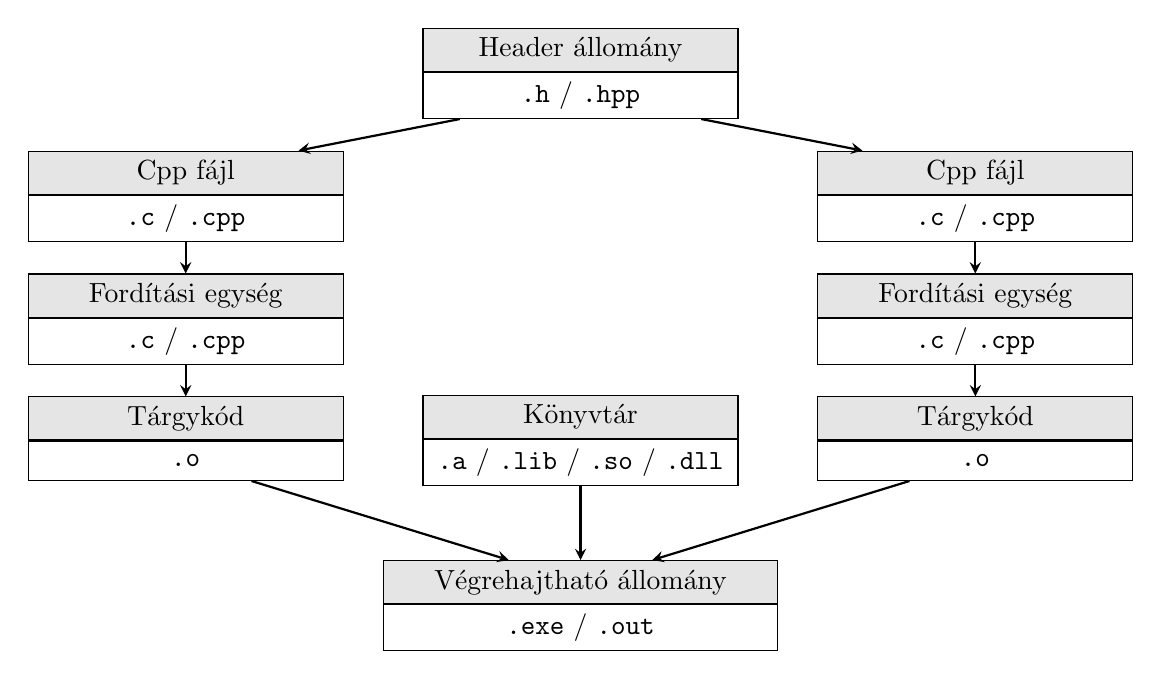
\begin{tikzpicture}
			\tikzstyle{Node} = [rectangle, minimum width=4cm, minimum height=5mm, text centered, draw=black, fill= gray!20]
			\tikzstyle{FileName} = [rectangle, minimum width=4cm, minimum height=5mm, text centered, draw=black, fill= white]
			\tikzstyle{NodeExe} = [rectangle, minimum width=5cm, minimum height=5mm, text centered, draw=black, fill= gray!20]
			\tikzstyle{FileNameExe} = [rectangle, minimum width=5cm, minimum height=5mm, text centered, draw=black, fill= white]
			\tikzstyle{arrow} = [thick,->,>=stealth]
			
			
			\node (header) [Node] {Header állomány};
			\node (headerFileName) [FileName, below = 0mm of header] {\texttt{.h} / \texttt{.hpp}};
			
			\node (cpp1) [Node, below left = of header] {Cpp fájl};
			\node (cpp1FileName) [FileName, below = 0mm of cpp1] {\texttt{.c} / \texttt{.cpp}};
			
			\node (cpp2) [Node, below right = of header] {Cpp fájl};
			\node (cpp2FileName) [FileName, below = 0mm of cpp2] {\texttt{.c} / \texttt{.cpp}};
			
			\node (translationUnit1) [Node, below = of cpp1] {Fordítási egység};
			\node (translationUnit1FileName) [FileName, below = 0mm of translationUnit1] {\texttt{.c} / \texttt{.cpp}};
			
			\node (translationUnit2) [Node, below = of cpp2] {Fordítási egység};
			\node (translationUnit2FileName) [FileName, below = 0mm of translationUnit2] {\texttt{.c} / \texttt{.cpp}};
			
			\node (objectFile1) [Node, below = of translationUnit1] {Tárgykód};
			\node (objectFile1FileName) [FileName, below = 0mm of objectFile1] {\texttt{.o}};
			
			\node (objectFile2) [Node, below = of translationUnit2] {Tárgykód};
			\node (objectFile2FileName) [FileName, below = 0mm of objectFile2] {\texttt{.o}};
			
			
			\node (libFile1) [Node, below = 4.1 cm of header] {Könyvtár};
			\node (libFile1FileName) [FileName, below = 0mm of libFile1] {\texttt{.a} / \texttt{.lib} / \texttt{.so} / \texttt{.dll}};
			
			\node (exe) [NodeExe, below = 6.2 cm of header] {Végrehajtható állomány};
			\node (exeFileName) [FileNameExe, below = 0mm of exe] {\texttt{.exe} / \texttt{.out}};
			
			
			\draw[arrow] (headerFileName) -- (cpp1);
			\draw[arrow] (headerFileName) -- (cpp2);
			\draw[arrow] (cpp1FileName) -- (translationUnit1);
			\draw[arrow] (cpp2FileName) -- (translationUnit2);
			\draw[arrow] (translationUnit1FileName) -- (objectFile1);
			\draw[arrow] (translationUnit2FileName) -- (objectFile2);
			\draw[arrow] (objectFile1FileName) -- (exe);
			\draw[arrow] (objectFile2FileName) -- (exe);
			\draw[arrow] (libFile1FileName) -- (exe);
			%TODO lehet az utolsó két oszlopot fel kéne cserélni
		\end{tikzpicture}
		\smallskip
		
		Szürkében az adott fordítási lépés neve, alatta az így létrehozott fájl kiterjesztése (leggyakrabban).
	\end{figure}
	A fordítás a preprocesszor parancsok végrehajtásával kezdődik (például a \textbf{header fájl}ok beillesztése a \textbf{cpp fájl}okba), az így kapott fájlot hívjuk \textbf{fordítási egység}nek (\textit{translation unit}). A fordítási egységek külön-külön fordulnak \textbf{tárgykód}dá (\textit{object file}). Ahhoz hogy a tárgykódokból \textbf{futtatható állomány}t (\textit{executable file}) lehessen készíteni, össze kell linkelni őket. A saját forráskódunkból létrejövő tárgykódok mellett a linker a felhasznált könyvtárak tárgykódjait is bele fogja szerkeszteni a végleges futtatható állományba.
	\medskip
	
	A következő pár szekcióban megismerjük a fenti 3 lépést alaposabban.
	
	\subsection{Preprocesszálás}
	A preprocesszor (vagy előfeldolgozó) használata a legtöbb esetben kerülendő. Ez alól kivétel a header állományok include-olása. A preprocesszor \textbf{primitív} szabályok alapján dolgozik és \textbf{nyelvfüggetlen.} Mivel semmit nem tud a C++-ról, ezért sokszor a fejlesztő számára meglepő viselkedést okozhat a használata. Emellett nem egyszerű diagnosztizálni a preprocesszor használatából származó hibákat. További probléma, hogy az automatikus refaktoráló eszközök használatát is megnehezíti a preprocesszor túlhasználata.
	
	A következőkben néhány preprocesszor direktívával fogunk megismerkedni. Minden direktíva \texttt{\#} jellel kezdődikcl. Ezeket a sorokat a fordító a program fordítása szempontjából figyelmen kívül hagyja.
  \bigskip
	
	\fbox{\textbf{alma.h}}
	\begin{lstlisting}
#define ALMA 5

ALMA ALMA ALMA
	\end{lstlisting}
	A \texttt{\#define ALMA 5}  parancs azt jelenti, hogy minden \texttt{ALMA} szót ki kell a fájlban \texttt{5}-re.
	
	Az előfeldolgozott szöveget a \texttt{cpp alma.h} parancs kiadása segítségével tekinthetjük meg.
	
	Az így kapott fájlból kiolvasható előfeldolgozás eredménye: \texttt{5 5 5}.
	\bigskip
	
	\fbox{\textbf{alma.h}}
	\begin{lstlisting}
#define KORTE

#ifdef KORTE
	MEGVAN
#else
	KORTE
#endif
	\end{lstlisting}
	A fent leírtakon kívül a \texttt{\#define} hatására a preprocesszor az első argumentumot makrónak fogja tekinteni. A fenti kódban rákérdezünk, hogy ez a \texttt{KORTE} makró definiálva van-e (az \texttt{\#ifdef} paranccsal), és mivel ezt fent megtettük, \texttt{\#else}-ig (vagy annak hiányában \texttt{\#endif}-ig) minden beillesztésre kerül, kimenetben csak annyi fog szerepelni, hogy \texttt{MEGVAN}.
	\bigskip
	
	\fbox{\textbf{alma.h}}
	\begin{lstlisting}
#define KORTE
#undef KORTE

#ifdef KORTE
	MEGVAN
#else
	KORTE
#endif
	\end{lstlisting}
	Az \texttt{\#undef} paranccsal a paraméterként megadott makrót a preprocesszor nem tekinti továbbá makrónak, így a kimenetben \texttt{KORTE} lesz.
	
	Látható, hogy az előfeldolgozót kódrészletek kivágására is lehet használni. 
  Felmerülhet a kérdés, ha az eredeti forrásszövegből az előfeldolgozó kivág illetve beilleszt részeket, akkor a fordító honnan tudja, hogy a hiba jelentésekor melyik sorra jelezze a hibát? Hiszen az előfeldolgozás előtti és utáni sorszámok egymához képest eltérnek. Ennek a problémának a megoldására az előfeldolgozó beszúr a fordító számára plusz sorokat, amik hordozzák azt az információt, hogy a feldolgozás előtt az adott sor melyik fájl hányadik sorában volt megtalálható. 
	\begin{note}
		 A fordítás közbeni ideiglenes fájlokat a \texttt{g++ -save-temps hello.cpp} paranccsal lehet lementeni.
	\end{note}
	A már bizonyára ismerős \texttt{\#include} egy paraméterént megadott fáj tartalmát illeszti be egy az egyben az adott fájlba, és így nagyon jelentősen meg tudják növelni a kód méretét, ami a fordítást lassítja. Ezért óvatosan kell vele bánni.
	\bigskip
	
	\fbox{\textbf{pp.h}}
	\begin{lstlisting}
#include "pp.h"
	\end{lstlisting}
		
	Rekurzív include-nál, mint a fenti példában, az előfeldolgozó egy bizonyos mélységi limit után leállítja a preprocesszálást.
	
	Sok és hosszú include láncok esetén azonban nehéz megakadályozni, hogy kör kerüljön az include gráfba, így akaratlanul is a rekurzív include-ok aldozatai lehetünk.
	\bigskip
	
	\fbox{\textbf{pp.h}}
	\begin{lstlisting}
#ifndef _PP_H_
#define _PP_H_

	FECSKE

#endif
	\end{lstlisting}
	
	\fbox{\textbf{alma.h}}
	\begin{lstlisting}
#include "pp.h"
#include "pp.h"
#include "pp.h"
#include "pp.h"
#include "pp.h"
	\end{lstlisting}
	
	Egy trükk segítségével megakadályozhatjuk azt, hogy többször be legyen illesztve \texttt{FECSKE}. Először megnézzük, hogy \texttt{\_PP\_H\_} szimbólum definiálva van-e. Ha nincs, definiáljuk. Mikor legközelebb ezt meg akarnánk tenni (a második \texttt{\#include "pp."} sornál), nem illesztjük be a \texttt{FECSKE}-t, mert \texttt{\#ifndef \_PP\_H\_} kivágja azt a szövegrészt.
	
	Ez az úgy nevezett \textbf{header guard} vagy \textbf{include guard.}
	
	\medskip
	A preprocesszor az itt bemutatottaknál sokkal többet tud, de általában nem érdemes túlhasználni a fent említett okok miatt.
	
	\subsection{Linkelés}
	\bigskip
	
	\fbox{\textbf{fecske.cpp}}
	\begin{lstlisting}
void fecske() {}
	\end{lstlisting}
	\bigskip
	
	\fbox{\textbf{main.cpp}}
	\begin{lstlisting}
int main()
{
	fecske();
}
	\end{lstlisting}
		
	Ez nem fog lefordulni, mert vagy csak a main.cpp-ből létrejövő fordítási egységet, vagy a fecske.cpp-ből létrejövő fordítási egységet látja a fordító, egyszerre a kettőt nem. Megoldás az ha \textbf{forward deklarálunk}, \texttt{void fecske();}-t beillesztjük a main függvény fölé, mely jelzi a fordítónak, hogy a \texttt{fecske} az egy függvény, \texttt{void} a visszatérési értéke és nincs paramétere. 
	\medskip
	
	Ekkor \texttt{g++ main.cpp} paranccsal történő fordítás a linkelési fázisánál kapunk hibát, mert nem találja a \texttt{fecske} függvény definícióját. Ezt ahogy korábban láttuk, úgy tudjuk megoldani, ha \texttt{main.cpp}-ből és \texttt{fecske.cpp}-ből is tárgykódot készítünk, majd összelinkeljük őket. \texttt{main.cpp}-ben lesz egy hivatkozás egy olyan \texttt{fecske} függvényre, melynek \texttt{void} a visszatérési értéke és paramétere nincs, és \texttt{fecske.cpp} fogja tartalmazni e függvény definícióját. 
		
    {\centering\texttt{g++ -c main.cpp}\par}

	{\centering\texttt{g++ -c fecske.cpp}\par}

	A fenti paranccsal lehet tárgykódot előállítani.
	
	{\centering\texttt{g++ main.o fecske.o}\par}
	
	Ezzel a paranccsal pedig az eredményül kapott tárgykódokat lehet összelinkelni. Rövidebb, ha egyből a cpp fájlokat adjuk meg a fordítónak, így ezt a folyamatot egy sorral letudhatjuk..

	{\centering\texttt{g++ main.cpp fecske.cpp} \par}
	
	Ha a \texttt{fecske.cpp}-ben sok függvény van, akkor nem célszerű egyesével forward deklarálni őket minden egyes fájlban, ahol használni szeretnénk ezeket a függvényeket. Ennél egyszerűbb egy header fájl megírása, amiben deklaráljuk a \texttt{fecske.cpp} függvényeit.
	\bigskip
	
	\fbox{\textbf{fecske.h}}
	\begin{lstlisting}
#ifndef _FECSKE_H_
#define _FECSKE_H_
	void fecske();
#endif
	\end{lstlisting}
	Ilyenkor elég a \texttt{fecske.h}-t includeolni.
	\medskip
	
	\textbf{Függvény definíció}nak nevezzük azt, amikor megmondjuk a függvénynek hogy mit csináljon. Ez egyben deklaráció is, hiszen a paraméterekről és visszatérési értékekről is tartalmazza a szükséges információkat.
	\medskip
	
	\textbf{Függvény deklaráció}nak nevezzük azt, amikor függvény használatáról adunk információt. A paraméterek típúsáról, visszatérési értékről és a függvény nevéről.
	\medskip
	
  Szokás a fecske.h-t a fecske.cpp-be is includeolni, mert ha véletlenül ellent mondana egymásnak a definíció a cpp fájlban és a deklaráció a header fájlban akkor a fordító hibát fog jelezni. (Például ha eltérő visszatérési érték típust adtunk meg a definíciónak a C++ fájlban és a deklarációnak a header fájlban.)
	
	Valami akárhányszor deklarálhatunk, azonban ha a deklarációk ellentmondanak egymásnak, akkor fordítási hibát kapunk. Definiálni viszont mindent pontosan egyszer kell. Több definíció vagy a definíció hiánya problémát okozhat. Ezt az elvet szokás \textbf{One Definition Rule}-nak, vagy röviden \textbf{(ODR)}-nek hívni.
	\bigskip
	
	\fbox{\textbf{fecske.h}}
	\begin{lstlisting}
#ifndef _FECSKE_H_
#define _FECSKE_H_
	void fecske();
	int macska() {}
#endif
	\end{lstlisting}
		
	Ha több fordítási egységből álló programot fordítunk, melyek tartalmazzák a \texttt{fecske.h} headert, akkor a preprocesszor több macska függvény definíciót csinál, és linkeléskor a linker azt látja, hogy egy függvény többször van definiálva, és ez linkelési hibát eredményez.
	\begin{note}
		A header fájlokba nem szabad definíciókat rakni (bár kivétel létezik, pl. template-ek, inline függvények, melyekről később lesz szó).
	\end{note}
	
	\section{Figyelmeztetések}

  A fordító gyanús vagy hibás kódrészlet esetén tud figyelmeztetéseket generálni. A legtöbb fordító alapértelmezetten elég kevés hibalehetőségre figyelmeztet. További figyelmeztetések bekapcsolásával hamarabb, már fordítási időben megtalálhatunk bizonyos hibákat vagy nem definiált viselkedéseket. Ezért ajánlott a \texttt{-Wall}, \texttt{-Wextra} kapcsolókat használni.

	{\centering \texttt{g++ -Wall -Wextra hello.cpp} \par}

	\section{Optimalizálás}
	A fordításnál bekapcsolhatunk optimalizációkat, a GCC-nél pl. így:
	
	{\centering \texttt{g++ hello.cpp -O2} \par}
	
	Az \texttt{-O2} paraméter a kettes szintű optimalizációk kapcsolja be. Alapértelmezetten nincs optimalizáció (\texttt{-O0}), és egészen \texttt{-O3}-ig lehet fokozni azt.
	\bigskip
	
	\fbox{\textbf{hello.cpp}}
	\begin{lstlisting}
int factorial(int n)
{
	if (n <= 0) return 1;
	else return n*factorial(n-1);
}

int main()
{
	std::cout << factorial(5) << std::endl;
}
	\end{lstlisting}
	
	A \texttt{g++ -save-temps hello.cpp} paranccsal fordítva a temporális fájlokat is meg tudjuk nézni -- hello.s lesz az assembly fájl neve, mely a fordító a kódunk alapján generált. Kiolvasható benne ez a két sor:
	\begin{lstlisting}
movl 	$5, (%esp)
call	__Z9factoriali
	\end{lstlisting}
	\begin{note}
		Az, hogy a fordító milyen assembly kódot alkot az input fájlból, implementációfüggő, ebben az esetben ezt az eredményt kaptuk.
	\end{note}
	Látható, hogy a \texttt{factorial} függvény 5 paraméterrel meg lett hívva (az hogy pontosan itt mi történik, az lényegtelen).
	
	\medskip
	Amennyiben azonban \texttt{g++ -save-temps hello.cpp -O2} paranccsal fordítunk, az optimalizált assembly kódból kiolvasható, hogy a kód (kellően friss gcc-vel) a faktoriális kiszámolása helyett a végeredményt (120at) tartalmazza. 
	\begin{lstlisting}
movl	$120, (%esp)
	\end{lstlisting}
	Így, mivel az eredmény már fordítási időben kiszámolásra került, futási időben nem kell ezzel plusz időt tölteni.
	
	A fordító sok ehhez hasonló \textbf{optimalizációt} végez. Ennek hatására a szabványos és csak definiált viselkedést tartalmazó kód jelentése nem változhat, viszont sokkal hatékonyabbá válhat.
	\begin{note}
		\texttt{-O3} Olyan optimalizálásokat is tartalmazhat, amik agresszívabban kihasználják, ha egy kód nem definiált viselkedéseket tartalmaz, míg az\texttt{-O2} kevésbé aggresszív, sokszor a nem szabványos kódot se rontja el. Mivel nem definiált viselkedésekre rosszul tud reagálni az \texttt{-O3}, így néha kockázatos használni.
	\end{note}
	\section{Globális változók}
	\subsection{Féligazságok előzménytárgyakból}
	Előzménytárgyakból azt tanultuk, hogy a program futása a main függvény végrehajtásával kezdődik. Biztosan igaz ez?
	\begin{lstlisting}
std::ostream& os = std::cout << "Hello";
int main()
{
	std::cout << "valami";
}
	\end{lstlisting}
	Kimenet: \texttt{Hellovalami}.
	\medskip
	
	Tehát ez nem volt igaz. A program végrehajtásánál az első lépés az un. \textbf{globális változók} inicializálása. 
	
	Ennek az oka az, hogy a globális változók olyan objektumok, melyekre a program bármely pontján hivatkozni lehet, így ha \texttt{os}-t akarnám használni a \texttt{main} függvény első sorában, akkor ezt meg lehessen tenni. Inicializálatlan változó használata pedig nem definiált viselkedés, ezért fontos már a \texttt{main} végrehajtása előtt inicializálni a globálisokat.
	\begin{lstlisting}
int f()
{
	return 5;
}

int x = f();

int main()
{
	std::cout << "valami";
}
	\end{lstlisting}
	Itt szintén az \texttt{f()} kiértékelése a \texttt{main} függvény meghívása előtt történik, hogy a globális változót létre lehessen hozni.
	%TODO névtelen névtér
	\subsection{Globális változók definíciója és deklarációja}
	Globális változókat úgy tudunk létrehozni, hogy közvetlen egy névteren belül (erről később) definiáljuk őket.
	\medskip
	
	\fbox{\textbf{main.cpp}}
	\begin{lstlisting}
int x;

int main() {}
	\end{lstlisting}
	\texttt{x} egy globális változó. Azonban mit tudunk tenni, ha nem csak a \texttt{main.cpp}-ben, hanem egy másik fordítási egységben is szeretnénk rá hivatkozni?
	\medskip
	
	\fbox{\textbf{other.cpp}}
	\begin{lstlisting}
int x;

void f() 
{
	x = 0;
}
	\end{lstlisting}
  Sajnos ha \texttt{main.cpp}-t és \texttt{other.cpp}-t együtt fordítjuk, fordítási hibát kapunk, ugyanis megsértettük az ODR-t, hiszen \texttt{x} kétszer van definiálva. Ezt úgy tudjuk megoldani, ha \texttt{x}-et forward deklaráljuk az \texttt{extern} kulcsszóval!
	\medskip
	
	\fbox{\textbf{other.cpp}}
	\begin{lstlisting}
extern int x;

void f() 
{
	x = 0;
}
	\end{lstlisting}
	Csupán annyi a fontos, hogy \texttt{x}-et valamikor definiálni is kell (mely jelenleg a \texttt{main.cpp}-bentalálható).
	\begin{note}
		A globális változók deklarációit érdemes külön header fájlba kigyűjteni.
	\end{note}
	\subsection{Globális változók inicializációja}
	A globális változók egyedi módon kapnak kezdőértéket (inicializálódnak). Amennyiben egy nem globális \texttt{int}-et hozunk létre és nem adunk neki kezdőértéket, annak értéke nem definiált lesz (memóriaszemét).
	\begin{lstlisting}
int i;

int main() 
{
	std::cout << i << std::endl; // 0
}
	\end{lstlisting}   
	Azonban mégis mindig 0-t fog ez a program kiírni. Ennek oka az, hogy a globális változók mindig 0-ra inicializálódnak (legalábbis az \texttt{int}-ek). A globális változókat csak egyszer hozzuk létre a program futásakot, így érdemes jól definiált kezdőértéket adni neki.
	
	Azonban a stacken (mellyel hamarosan megismerkedünk) rengetegszer létre kell hozni változókat, nem csak egyszer, így ott nem éri meg minden alkalommal egy jól definiált kezdőértékkel inicializálni. Sokkal nagyobb lenne a hatása a futási időre.
	
	Annak, hogy miért épp 0-ra inicializálódnak a globális változók, az az oka, hogy ezt a modern processzorok gyorsan tudják kivitelezni minden platformon. 
	\subsection{Problémák a globális változókkal}
	
	A linkelés vajon befolyásolhatja a program megfigyelhető viselkedését?
	\bigskip
	
	\fbox{\textbf{main.cpp}}
	\begin{lstlisting}
std::ostream& o = std::cout << "Hello";
int main() {}
	\end{lstlisting}
	\bigskip
	
	\fbox{\textbf{fecske.cpp}}
	\begin{lstlisting}
std::ostream& o2 = std::cout << " World";
	\end{lstlisting}
	Itt nem specifikált a két globális változók inicializációs sorrendje, és ha más sorredben linkeljük a fordítási egységekből keletkező tárgykódot, mást ír ki.
	
	{\centering \texttt{g++ main.cpp fecske.cpp \quad $\not=$\quad\, g++ fecske.cpp main.cpp} \par}
	
	\begin{note}
		Ez utolsó példa nem számít jó kódnak, mert nem specifikált viselkedést használ ki. A program kimenete nem definiált. Ez is egy jó elrettentő példa, miért nem érdemes globális változókat használni.
	\end{note}
	
	Ezen kívül számos egyéb problémát is felvetnek a globális változók: túlzott használatuk a sok paraméterrel rendelkező függvények elkerülése végett fordulhat elő, azonban gyakran így sokkal átláthatatlanabb kódot kapunk. Mivel bárhol hozzá lehet férni egy globális változóhoz, nagyon nehéz tudni, mikor hol módosul.
	\begin{note}
    Párhuzamos programozásnál a globális változók túl az átláthatatlanságon még sokkal több fejtörést okoznak: mi van akkor, ha két párhuzamosan futó függvény ugyanazt a változót akarja módosítani? Ennek megelőzése globális változóknál ezt rendkívül körülményes lehet. A naív megoldás (kölcsönös kizárás) pedig rosszul skálázódó programot eredményez.
	\end{note}
	\section{Láthatóság, élettartam}
	Egy objektum \textbf{láthatóságának} nevezzük a kódnak azon szakaszait, melyeknél lehet rá hivatkozni.
	\smallskip
	
	Egy objektum \textbf{élettartamának} nevezzük a kód azon szakaszát, melynél bent szerepel a memóriában. Amikor egy objektum élettartama elkezdődik, azt mondjuk, az objektum létrejön, míg az élettartam végén az objektum megsemmisül.
	\medskip
	\begin{note}
		Ez alapján megállapíthatjuk, hogy egy globális változó láthatósága és élettartama a program futásának elejétől végéig tart.
	\end{note}
	
	Figyeljük meg, mikor tudunk \texttt{x} változóra hivatkozni (azaz hol lesz \texttt{x} látható)!
	\begin{lstlisting}
int x;

int main()
{
	int x = 1;
	{
		int x = 2;
		std::cout << x << std::endl; // 2
	}
}
	\end{lstlisting}
	Megfigyelhető, hogy a \texttt{main} függvény elején létrehozott \texttt{x} az utána következő blokkban teljesen elérhetetlen -- nincs olyan szabványos nyelvi eszköz, amivel tudnánk rá hivatkozni. Ezt a folyamatot \textbf{leárnyékolás}nak (\textit{shadowing}) nevezzük. Azonban a külső, globális \texttt{x}-re bármikor tudunk hivatkozni az alábbi módon:
	\begin{lstlisting}
int x;

int main()
{
	int x = 1;
	{
		int x = 2;
		std::cout << ::x << std::endl; // 0
	}
}
	\end{lstlisting}
	
	\section{A stack működése}
	A stack a C++ alapértelmezett tárolási osztálya lokális változók esetén: minden változó alapértelmezetten itt jön létre és semmisül meg. Az itt létrejött változók automatikusan megsemmisülnek. Az élettartamuk a definíciójuktól az adott blokk végéig tart.
	
	\begin{lstlisting}
#include <iostream>

int f()
{
	int x = 0; //x letrejon
	++x;
	return x;
} //x megsemmisul

int main()
{
	for (int i = 0; i<5; i++)
		std::cout << f() << ' '; // 1 1 1 1 1
}
	\end{lstlisting}
	\medskip
	
	A fenti kód futása során a stack-et így képzelhetjük el:
	
	\begin{figure}[!h]
		\centering
		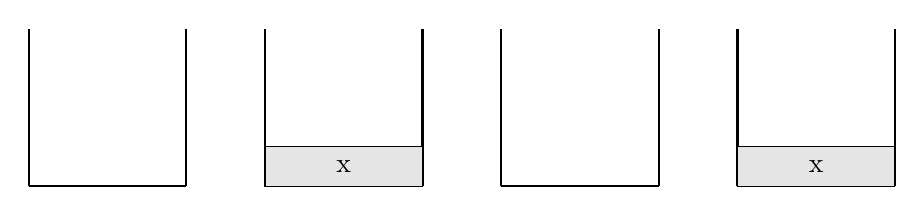
\begin{tikzpicture}
		\tikzstyle{Node} = [rectangle, minimum width=2cm, minimum height=5mm, text centered, draw=black, fill= gray!20]
		\tikzstyle{arrow} = [thick,->,>=stealth]
		
		
		\draw [thick, black] (-3, 0) -- (-1, 0);
		\draw [thick, black] (-3, 0) -- (-3, 2);
		\draw [thick, black] (-1, 0) -- (-1, 2);
		
		\draw [thick, black] (0, 0) -- (2, 0);
		\draw [thick, black] (0, 0) -- (0, 2);
		\draw [thick, black] (2, 0) -- (2, 2);
		\node (x) [Node] at (1,0.25) {x};
		
		\draw [thick, black] (3, 0) -- (5, 0);
		\draw [thick, black] (3, 0) -- (3, 2);
		\draw [thick, black] (5, 0) -- (5, 2);
		
		\draw [thick, black] (6, 0) -- (8, 0);
		\draw [thick, black] (6, 0) -- (6, 2);
		\draw [thick, black] (8, 0) -- (8, 2);
		\node (x) [Node] at (7,0.25) {x};
		\end{tikzpicture}
	\end{figure}
	Az ábrán egy stack-et látunk. Amikor a vezérlés az \texttt{f} függvényhez ér, és ott létrehozza az \texttt{x} változót, azt behelyezi a stack-be. A \texttt{return} kulcsszó hatására készít \texttt{x}-ről egy temporális példányt, ami a függvény visszatérési értéke lesz. Amikor a vezérlés visszatér a \texttt{main} függvényhez, {x}-re nem tudunk tovább hivatkozni, így azt megsemmisíti, és ez ismétlődik, ameddig a ciklus véget nem ér.
	\smallskip
	
	A stack egy FILO (\textit{first in last out}) adatszerkezet -- azaz azt az elemet ,,dobja'' ki a vezérlés a stack-ből, melyet utoljára rakott be.
	
	\section{Paraméter átvétel}
	\subsection{Érték szerinti paraméter átvétel}
	Próbáljuk megvalósítani a swap függvényt!
	%http://tex.stackexchange.com/questions/228724/how-do-i-make-tikz-make-a-curved-arrow-from-one-node-to-another-when-my-nodes-ar
	\begin{lstlisting}
#include <iostream>
void swapWrong(int a, int b)
{
	int tmp = a;
	a = b;
	b = tmp;
}

int main()
{
	int c = 5, d = 8;
	swapWrong(c, d);
	std::cout << c << ' ' << d << std::endl;
}
	\end{lstlisting}		
	A program kimenete \texttt{5 8}. Ez egy teljesen jól definiált viselkedés. Ennek az az oka, hogy itt \textbf{érték} szerint vettük át (\textit{pass by value}) \texttt{a} és \texttt{b} paramétert. A következő ábrán megfigyelhetjük mi is történik pontosan. Képzeljük el, hogy a stackbe a program elrakja a \texttt{c} és \texttt{d} változókat. Eztán meghívja a \texttt{swapWrong} függvényt, melyben létrehozott \texttt{a} és \texttt{b} paraméterek szintén a stackre kerülnek. Bár a függvényre lokális \texttt{a} és \texttt{b} paraméterek értékét megcseréli, de a függvényhívás után ezeket ki is törli a stackből. Az eredeti \texttt{c} és \texttt{d} változók éréke nem változott a függvényhívás során.
	\begin{figure}[!h]
		\centering
		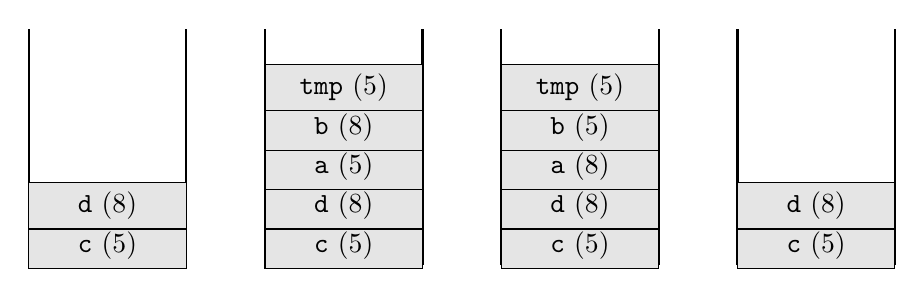
\begin{tikzpicture}
		\tikzstyle{Node} = [rectangle, minimum width=2cm, minimum height=5mm, text centered, draw=black, fill= gray!20]
		\tikzstyle{arrow} = [thick,->,>=stealth]
		
		\draw [thick, black] (0, 0) -- (2, 0);
		\draw [thick, black] (0, 0) -- (0, 3);
		\draw [thick, black] (2, 0) -- (2, 3);
		\node (c2) [Node] at (1,0.25) {\texttt{c} (5)};
		\node (d2) [Node] at (1,0.75) {\texttt{d} (8)};
		
		\draw [thick, black] (3, 0) -- (5, 0);
		\draw [thick, black] (3, 0) -- (3, 3);
		\draw [thick, black] (5, 0) -- (5, 3);
		\node (c3) [Node] at (4,0.25) {\texttt{c} (5)};
		\node (d3) [Node] at (4,0.75) {\texttt{d} (8)};
		\node (a3) [Node] at (4,1.25) {\texttt{a} (5)};
		\node (b3) [Node] at (4,1.75) {\texttt{b} (8)};
		\node (b3) [Node] at (4,2.25) {\texttt{tmp} (5)};
		
		\draw [thick, black] (6, 0) -- (8, 0);
		\draw [thick, black] (6, 0) -- (6, 3);
		\draw [thick, black] (8, 0) -- (8, 3);
		\node (c3) [Node] at (7,0.25) {\texttt{c} (5)};
		\node (d3) [Node] at (7,0.75) {\texttt{d} (8)};
		\node (a3) [Node] at (7,1.25) {\texttt{a} (8)};
		\node (b3) [Node] at (7,1.75) {\texttt{b} (5)};
		\node (b3) [Node] at (7,2.25) {\texttt{tmp} (5)};
		
		\draw [thick, black] (9, 0) -- (11, 0);
		\draw [thick, black] (9, 0) -- (9, 3);
		\draw [thick, black] (11, 0) -- (11, 3);
		\node (a4) [Node] at (10,0.25) {\texttt{c} (5)};
		\node (b4) [Node] at (10,0.75) {\texttt{d} (8)};
		\end{tikzpicture}
		\smallskip
	\end{figure}
	C++ban alapértelmezett módon a paraméterátadás érték szerint történik.
	\subsection{Mutatók érték szerinti átadása}
	A mutatók olyan nyelvi elemek, melyek egy adott típusú memóriaterületre mutatnak. Segítségükkel anélkül is tudunk hivatkozni egy adott objektumra (és nem csak a másolatára), hogy közvetlenül az objektummal dolgoznánk. Most röviden megismerkedünk velük, de később részletesebben visszatérünk rájuk.
	\begin{lstlisting}
int main()
{
	int c = 5, d = 8;
	int *p = &c;
}
	\end{lstlisting}
	A fenti példában \texttt{p} egy mutató (\textit{pointer}), mely egy \texttt{int} típusra mutat. Ahhoz, hogy értéket tudjunk adni egy mutatónak, egy memóriacímet kell neki értékül adni, erre való a \textbf{címképző operátor} (\&). Ha a mutató által \textit{mutatott értéket} szeretnénk módosítani, akkor dereferálnunk kell a \textbf{dereferáló operátor}ral (*).
	\begin{lstlisting}
int *p = &c; //referaljuk c-t
*p = 4; //dereferaljuk p-t
p = &d;
*p = 7;
	\end{lstlisting}
	Rendre: pointer inicializálása, pointer által mutatott érték módosítása, pointer átállítása másik memóriacímre, és a mutatott érték módosítása.
	
	Egy mutató mutathat változóra, másik mutatóra vagy sehova. Azokat a mutatókat, melyek sehová sem mutatnak, null pointernek nevezzük, és így hozhatjuk létre őket:
	
	{\centering \texttt{p = 0;\quad \quad p = NULL;\quad \quad p = nullptr;} \par}
	
	\begin{note}
		Ez a három értékadás (közel) ekvivalens, azonban a \texttt{nullptr} kulcsszó csak C++11ben és azutáni szabványokban érhető el.
	\end{note}

  Nézzük meg, hogy hogyan tudunk megcserélni két értéket ezúttal helyesen, mutatók segítségével.
	
	\begin{lstlisting}
void swapP(int *a, int *b)
{
	int tmp = *a;
	*a = *b;
	*b = tmp;
}
	\end{lstlisting}
	
	Amennyiben ezt a függvényt hívjuk meg, valóban megcserélődik a két változó értéke. De ehhez fontos, hogy ne \texttt{swapP(c, d)}-t írjunk, az ugyanis az fordítási hibához vezetne, hiszen a \texttt{c} és \texttt{d} típusa \texttt{int}, és nem \texttt{int*}. Ahhoz, hogy értéket adjunk egy pointernek, a \texttt{c}-hez és \texttt{d}-hez tartozó memóriacímeket kell átadni, így a \texttt{swapP(\&c, \&d)} hívás lesz megfelelő.
	\begin{note}
    A mutatókat továbbra is érték szerint adjuk át. Az \texttt{a} és \texttt{b} paraméterekben lévő memóriacím tehát a másolata annak, amit a hívás helyén megadtunk.
	\end{note}
	\begin{figure}[!h]
		\centering
		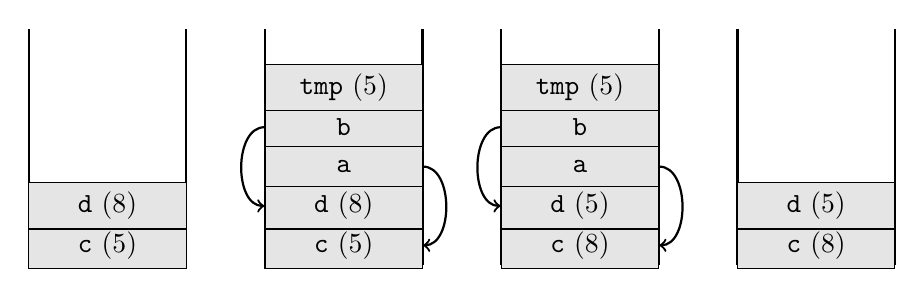
\begin{tikzpicture}
		\tikzstyle{Node} = [rectangle, minimum width=2cm, minimum height=5mm, text centered, draw=black, fill= gray!20]
		\tikzstyle{arrow} = [thick,->,>=stealth]
		
		\draw [thick, black] (-3, 0) -- (-1, 0);
		\draw [thick, black] (-3, 0) -- (-3, 3);
		\draw [thick, black] (-1, 0) -- (-1, 3);
		\node (c1) [Node] at (-2,0.25) {\texttt{c} (5)};
		\node (d1) [Node] at (-2,0.75) {\texttt{d} (8)};
		
		\draw [thick, black] (0, 0) -- (2, 0);
		\draw [thick, black] (0, 0) -- (0, 3);
		\draw [thick, black] (2, 0) -- (2, 3);
		\node (c2) [Node] at (1,0.25) {\texttt{c} (5)};
		\node (d2) [Node] at (1,0.75) {\texttt{d} (8)};
		\node (a2) [Node] at (1,1.25) {\texttt{a}};
		\node (b2) [Node] at (1,1.75) {\texttt{b}};
		\node (tmp2) [Node] at (1,2.25) {\texttt{tmp} (5)};
		
		\path[every node/.style={font=\sffamily\small}]
			(a2) edge[bend left = 90, thick, ->] node [right] {} (c2);
		\path[every node/.style={font=\sffamily\small}]
			(b2) edge[bend right = 90, thick, ->] node [left] {} (d2);
		
		\draw [thick, black] (3, 0) -- (5, 0);
		\draw [thick, black] (3, 0) -- (3, 3);
		\draw [thick, black] (5, 0) -- (5, 3);
		\node (c3) [Node] at (4,0.25) {\texttt{c} (8)};
		\node (d3) [Node] at (4,0.75) {\texttt{d} (5)};
		\node (a3) [Node] at (4,1.25) {\texttt{a}};
		\node (b3) [Node] at (4,1.75) {\texttt{b}};
		\node (tmp3) [Node] at (4,2.25) {\texttt{tmp} (5)};
		
		
		\path[every node/.style={font=\sffamily\small}]
		(a3) edge[bend left = 90, thick, ->] node [right] {} (c3);
		\path[every node/.style={font=\sffamily\small}]
		(b3) edge[bend right = 90, thick, ->] node [left] {} (d3);
		
		\draw [thick, black] (6, 0) -- (8, 0);
		\draw [thick, black] (6, 0) -- (6, 3);
		\draw [thick, black] (8, 0) -- (8, 3);
		\node (a4) [Node] at (7,0.25) {\texttt{c} (8)};
		\node (b4) [Node] at (7,0.75) {\texttt{d} (5)};
		\end{tikzpicture}
	\end{figure}
	
	\begin{lstlisting}
void swapWrong2(int *a, int *b)
{
	int *tmp = a;
	a = b;
	b = tmp;
}
	\end{lstlisting}
	Ebben a példában nem a pointerek által mutatott értéket, hanem magukat a pointereket cseréljük meg. Itt az fog történni, hogy a függvény belsejében \texttt{a} és \texttt{b} pointer másra fog mutatni. A mutatott értékek viszont nem változnak.
	
	\begin{figure}[!h]
		\centering
		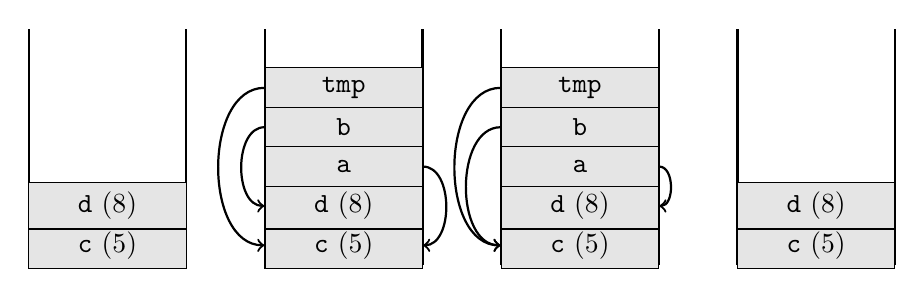
\begin{tikzpicture}
		\tikzstyle{Node} = [rectangle, minimum width=2cm, minimum height=5mm, text centered, draw=black, fill= gray!20]
		\tikzstyle{arrow} = [thick,->,>=stealth]
		
		\draw [thick, black] (-3, 0) -- (-1, 0);
		\draw [thick, black] (-3, 0) -- (-3, 3);
		\draw [thick, black] (-1, 0) -- (-1, 3);
		\node (c1) [Node] at (-2,0.25) {\texttt{c} (5)};
		\node (d1) [Node] at (-2,0.75) {\texttt{d} (8)};
		
		\draw [thick, black] (0, 0) -- (2, 0);
		\draw [thick, black] (0, 0) -- (0, 3);
		\draw [thick, black] (2, 0) -- (2, 3);
		\node (c2) [Node] at (1,0.25) {\texttt{c} (5)};
		\node (d2) [Node] at (1,0.75) {\texttt{d} (8)};
		\node (a2) [Node] at (1,1.25) {\texttt{a}};
		\node (b2) [Node] at (1,1.75) {\texttt{b}};
		\node (tmp2) [Node] at (1,2.25) {\texttt{tmp}};
		
		\path[every node/.style={font=\sffamily\small}]
		(a2) edge[bend left = 90, thick, ->] node [right] {} (c2);
		\path[every node/.style={font=\sffamily\small}]
		(b2) edge[bend right = 90, thick, ->] node [left] {} (d2);
		\path[every node/.style={font=\sffamily\small}]
		(tmp2) edge[bend right = 90, thick, ->] node [left] {} (c2);
		
		\draw [thick, black] (3, 0) -- (5, 0);
		\draw [thick, black] (3, 0) -- (3, 3);
		\draw [thick, black] (5, 0) -- (5, 3);
		\node (c3) [Node] at (4,0.25) {\texttt{c} (5)};
		\node (d3) [Node] at (4,0.75) {\texttt{d} (8)};
		\node (a3) [Node] at (4,1.25) {\texttt{a}};
		\node (b3) [Node] at (4,1.75) {\texttt{b}};
		\node (tmp3) [Node] at (4,2.25) {\texttt{tmp}};
		
		
		\path[every node/.style={font=\sffamily\small}]
		(a3) edge[bend left = 90, thick, ->] node [right] {} (d3);
		\path[every node/.style={font=\sffamily\small}]
		(b3) edge[bend right = 90, thick, ->] node [left] {} (c3);
		\path[every node/.style={font=\sffamily\small}]
		(tmp3) edge[bend right = 90, thick, ->] node [left] {} (c3);
		
		\draw [thick, black] (6, 0) -- (8, 0);
		\draw [thick, black] (6, 0) -- (6, 3);
		\draw [thick, black] (8, 0) -- (8, 3);
		\node (a4) [Node] at (7,0.25) {\texttt{c} (5)};
		\node (b4) [Node] at (7,0.75) {\texttt{d} (8)};
		\end{tikzpicture}
	\end{figure}
	\subsection{Referencia szerinti paraméter átadás}
	Megállapíthatjuk, hogy az előző megoldásnál nem változtattuk meg, hogy mire mutassanak a pointerek, így azokat konstansként is definiálhatnánk. A konstans pointerek módosíthatják a mutatott értéket, de nem lehet őket átállítani egy másik memória címre. Úgy tudunk egy ilyen pointert létrehozni, hogy a csillag után írjuk a \texttt{const} kulcsszót.
	\begin{lstlisting}
void swap(int * const a, int * const b)
{
	//...
}
	\end{lstlisting}
	Egy kis szintaktikai cukorkával megúszhatjuk azt, hogy folyton kiírjuk a \texttt{* const}-ot (lévén nem akarjuk megváltoztatni, hogy ilyen esetben a pointer hova mutasson). Erre való a {referencia szerinti paraméter átváétel} (\textit{pass by reference}). A referencia hasonlóan működik, mintha egy konstans pointer lenne, csak nem lehet sehova se mutató referenciát létrehozni.
	\begin{lstlisting}
void swapRef(int &a, int &b)
{
	int tmp = a;
	a = b;
	b = tmp;
}
	\end{lstlisting} 
  Ez a függvény lényegében ekvivalens a \texttt{swapP} fügvénnyel. 
	\begin{note}
		Ez bár ezt referencia szerinti átvételnek nevezzük, de itt is történik másolás, a memóriacímet ítt is érték szerint vesszük át.
	\end{note}
		Megjegyzendő, hogy a fenti \texttt{swapRef} függvény meghívásakor nem kell jeleznünk, hogy memóriacímeket akarunk átadni, \texttt{swapRef(a,b)}-t kell írnunk.
	\begin{note}
		Egy referenciát mindig inicializálni kell. Csak úgy mint egy konstanst (különben fordítási hibát kapunk.)
	\end{note}
	\subsection{Visszatérési érték problémája}
	Nem primitív (pl. \texttt{int}) típusoknál gyakran megeshet, hogy egy adott típushoz tartozó pointer mérete kisebb, mint magának az objektumé, így megérheti mindentől függetlenül a paramétert referencia szerint átvenni. Ezen felbátorodva mondhatnánk azt is, hogy referenciával is térjünk vissza (a követekező példában tekintsünk el attól, hogy \texttt{int}-el dolgozunk, bátran képzeljük azt hogy az pl. egy nagyon nagy mátrix)!
	\begin{lstlisting}
int& addOne(int &i)
{
	i++;
	return i;
}

int main()
{
	int i = 0;
	int a = addOne(i);
	std::cout << a << std::endl;
}
	\end{lstlisting}
	A fenti kóddal semmi gond nincs is. De mi van, ha egy picit módosítunk rajta?
	\begin{lstlisting}
int& addOne(int &i)
{
	int ret = ++i;
	return ret;
}
	\end{lstlisting}
	A baj máris megvan, amit egy warning is jelezni fog nekünk: olyan objektumra hivatkozó referenciát adunk vissza, amely \texttt{addOne}-on belül lokális. Ez azt jelenti, hogy amint a vezérlés visszatér a \texttt{main} függvényhez, \texttt{ret} megsemmisül, és a \texttt{main} függvény pedig a \texttt{ret}-hez tartozó címen lévő értéket próbálná meg lemásolni. Mivel viszont a \texttt{ret} már ezen a ponton megsemmisült, semmi nem garantálja, hogy azon a memóriaterületen ne követekezett volna be módosítás.
	
	\medskip
	Az olyan memóriaterületre való hivatkozás, mely nincs a program számára lefoglalva, nem definiált viselkedést eredményez.
	\begin{note}
		Értelemszerűen pointerekkel ez ugyanúgy probléma.
	\end{note}
	\section{Statikus változók/függvények}
	A \texttt{static} kulcsszónak számos jelentése van, annak függvényében, hogy milyen kontextusban írjuk egy változó vagy függvény elé. 
	\subsection{Fordítási egységre lokális változók}
	A függvényeken és osztályokon kívül deklarált statikus változók az adott fordítási egységre lokálisak -- élettartamuk a futás elejétől végigtartamig tart, és kizárólagosan az adott fordítási egységben láthatóak.
	\medskip
	
	\fbox{\textbf{main.cpp}}
	\begin{lstlisting}
#include <iostream>

static int x;

int main()
{
	x = 2;
}
	\end{lstlisting}
	\medskip
	
	\fbox{\textbf{other.cpp}}
	\begin{lstlisting}
#include <iostream>

static int x;

void f()
{
	x = 0;
}
	\end{lstlisting}
	Ha ezt a két fájlt együtt fordítjuk, nem kapunk linkelési hibát, ugyanis a \texttt{main.cpp}-ben lévő \texttt{x} egy teljesen más változó, mint ami az \texttt{other.cpp}-ben van.
	
	\smallskip
	Csak úgy mint a globális változókra, fordítási egységen belül bármikor hivatkozhatunk egy statikusra, és hasonló módon inicializálódnak.
	\begin{lstlisting}
static int x;

int main()
{
	int x = 4;
	std::cout << ::x << std::endl; // 0
}
	\end{lstlisting}
	\subsection{Függvényen belüli statikus változók}
	Azokat a változókat, melyek függvényen belül vannak a \texttt{static} kulcsszóval definiálva, függvényszintű változónak is szokás hívni. Élettartamuk a függvény első hívásától a program futásának végéig tart, míg láthatóságuk csak az adott függvényen belül van. A hagyományos lokális változókkal ellenben tehát nem semmisülnek meg, amikor az adott függvény futása befejeződik. A következő kódrészlet szemlélteti ezt a viselkedést.
	
	\begin{lstlisting}
int f()
{
	static int x = 0;
	++x;
	return x;
}

int main() 
{
	for(int i = 0; i<5; i++)
		std::cout << f() << ' '; // 1 2 3 4 5
}
	\end{lstlisting}
	Ahogy az megfigyelhető fent, \texttt{x} csak egyszer inicializálódik, majd a későbbi függvényhívások után egyre növekszik az értéke.
	\subsection{Fordítási egységre lokális függvények}
  Nem csak változókat, függvényeket is deklarálhatunk statikusnak, melyek a fordítási egységre lokálisak. Figyelem! Metódusok esetében mást jelent a \texttt{static} kulcsszó, mint amit itt leírtunk.
	\begin{lstlisting}
static int f()
{
	return 0;
}

int main() {std::cout << f();} // 0
	\end{lstlisting}
	Ezek a függvények csak az adott fordítási egységen belül érhetőek el.
	\subsection{Névtelen/anonim névterek}
	Fordítási egységre lokális változókat és függvényeket tudunk deklarálni névtelen névterek (\textit{unnamed namespaces}, vagy \textit{anonymous namespaces}) segítségével. Egy név nélküli névteren belül deklarált változók és függvények hasonlóan viselkednek, mintha eléjük lenne írva a \texttt{static} kulcsszó.
	\begin{lstlisting}
namespace
{
	int x;
	std::string y;
	void f() {}
}
	\end{lstlisting}
	\begin{note}
    A \texttt{static} osztályon belüli jelentéséről később lesz szó.
	\end{note}
	\section{Függvény túlterhelés}
	Térjünk vissza a korábban megírt swap függvényünkhöz.
	\begin{lstlisting}
void swap(int &a, int &b)
{
	int tmp = a;
	a = b;
	b = tmp;
}
	\end{lstlisting}
	Ez a függvény addig jó, amíg csak \texttt{int}-eket szeretnénk megcserélni. Mi van, ha \texttt{std::string}-eket kéne? A megoldás egyszerű, \textbf{túlterheljük} (\textit{overload}) a \texttt{swap} függvényt.
	\begin{lstlisting}
void swap(std::string &a, std::string &b)
{
	int tmp = a;
	a = b;
	b = tmp;
}
	\end{lstlisting}
	Túlterhelésnek azt nevezzük, amikor két vagy több függvénynek a neve azonos, de a paramétereik különböznek. Tagfüggvényeket konstansság alapján is túl lehet terhelni.
	\begin{note}
		A később elhangzó osztályok tagfüggvényeinél a függvény konstanssága is számít (azonos nevű és paraméter listájú függvény különöző konstanssággal ugyanúgy túlterhelésnek számít).
	\end{note}
	\subsection{Operátor túlterhelés}
	Ahogy láttuk a 2. gyakorlat elején, lehetőségünk van függvényeket túlterhelni. Ez operátorokra is igaz. Ha példaként vesszük a lineáris algebrából tanult rendezett valós számhármasokat ($\mathbb{R}^3$), lehetőségünk van arra, hogy a tanultak alapján definiáljuk a köztük értelmezett összeadást.
	%TODO temporális változók
	\begin{lstlisting}
struct LinAlgVector
{
	double x1, x2, x3;
};

LinAlgVector operator+(const LinAlgVector &lhs, const LinAlgVector &rhs)
{
	LinAlgVector ret;
	ret.x1 = lhs.x1 + rhs.x1;
	ret.x2 = lhs.x2 + rhs.x2; 
	ret.x3 = lhs.x3 + rhs.x3;
	return ret;
}

int main()
{
	LinAlgVector a, b;
	a.x1 = 1; a.x2 = 2; a.x3 = 3;
	b.x1 = 1; b.x2 = 1; b.x3 = 1;
	
	LinAlgVector c = a + b; 
}
	\end{lstlisting}
	A \texttt{main} függvényben lévő értékadás ezzel ekvivalens: \texttt{c = operator+(a, b)}, így láthatjuk, hogy az operátorok túlterhelése gyakorlatilag a függvénytúlterhelés speciális esete. 
	\smallskip 
	
	Írjuk meg a \texttt{print} függvényt 3D vektorokra! A gyakran kiíratáshoz használt jobb shift operátor (\textit{right shift operator}), a \texttt{\<} is túlterhelhető. Mivel mi az \texttt{std::cout} változóval szeretnénk majd kiíratni, melynek típusa \texttt{std::ostream}, így a függvényünk első paramétere egy ilyen típus lesz, a második meg egy \texttt{LinAlgVector} típus.
	
	\begin{lstlisting}
/* ... */

std::ostream& operator<<(std::ostream& os, const LinAlgVector &l)
{
	os << l.x1 << ' ' << l.x2 << ' ' << l.x3;
	return os;
}

int main()
{
	/* ... */
	std::cout << c << std::endl; // 2 3 4
}
	\end{lstlisting}
	
	Feltűnhet, hogy a stream objektumra mutató referenciát a függvény végén vissza is adjuk, hogy tudjuk a kiíratást láncolni.
%	\section{Kifejezések kiértékelése}
%	Ugorjunk vissza egy korábbi példára.
%	\begin{lstlisting}
%#include <iostream>
%
%int main()
%{
%	int i = 0;
%	std::cout << i << i++ << std::endl;
%}
%	\end{lstlisting}
%	%\< egy normálisabban kinéző << operátort eredményez (definíció fent)
%	
%	Világos, hogy a fenti kódban nem definiált viselkedés szerepel. Már volt szó arról is, hogy a kiíratáshoz használt \texttt{\<} szimbólum az egy operátor, és az \texttt{<iostream>} könyvtárban található hozzá egy olyan overload, melynek egyik paramétere \texttt{std::ostream\&}, a másik pedig \texttt{int}. Ahogy korábban is említve volt, az első paraméterével vissza is tér, így tudjuk a kiíratást láncolni. A fent leírt kiíratás ezzel lesz ekvivalens:
%	\begin{lstlisting}
%std::cout.operator<<(i).operator<<(i++);
%	\end{lstlisting}
%	
%	Itt látható egy \texttt{\<} operátor, ami így is felírható: \texttt{std::cout.operator$<<$(i)}. Ennek a függvényhívásnak van visszatérési értéke, méghozzá \texttt{std::cout}, így a függvényhívás láncolható. Ez itt egy member function, mellyel majdnem minden alaptípus  rendelkezik Ezalól kivétel a \texttt{std::string}, melynek \texttt{operator$>>$}-ja globális.
%	\begin{note}
%		Ennek az is lehet értelme, hogy ne függjön az operátor az osztálytól. Jó példa erre a \texttt{template}, mert annak csak akkor kell példányt létrehoznia, ha meghívják.
%	\end{note}
%	A fenti kódban lévő rész így is felírható:
%	
%	
%	Az, hogy a második szám 2 lesz, az biztos. De hogy az első mennyi, az nem definiált.
%	
%	\textit{1. ábra.}
%	
%	\begin{example}
%		\texttt{x = k + 2}\quad \quad \texttt{y = k + 2}
%	\end{example}
%	
%	Ebben a példában (jó eséllyel) a fordító kioptimalizálja ezt, és \texttt{k+2}-t csak egyszer számolja ki. A c++ban a nem szabványba foglalt szabályoknak köszönhetően sokkal hatékonyabb programokat kaphatunk, mert a fordítónak nagy szabadsága van abban, hogyan optimalizálja a kódunkat.
%	
%	\begin{example}
%		Itt a cél az lenne, hogy a tömb elemeit feltöltsük növekvő számokkal.
%		
%		\begin{lstlisting}
%int i = 0;
%int t[10];
%while (i < 10)
%{
%	t[i] = i++;
%}
%		\end{lstlisting}
%		
%		Azonban ez egy nem definiált viselkedés, mert hiába van ott egy \textbf{post-fix} \texttt{++}\quad operator, az hogy az egyenlőség melyik oldalán levő \texttt{i} értékelődik ki először, az ismét nem definiált.
%	\end{example}
%	
%	Itt leggyakrabban szekvenciapontok használata tud segíteni.
%	
%	\begin{definition}
%		(szekvenciapont) ami elválasztja, hogy mikor minek kell végrehajtódnia futási időben. A szekvenciapont előtt minden kifejezésnek ki kell értékelődnie. Több szekvenciapont létezik: vessző, \texttt{\&\&}, \texttt{||}, \texttt{?\quad :} 
%	\end{definition}
%	\begin{example}
%		\begin{lstlisting}
%f(i), ++i;
%i++<10 && f(i);
%i++<10 || f(i);
%i++<10 ? f(i) : g(i);
%		\end{lstlisting}
%		Ezek mint definiáltak, minden kifejezést egy szekvenkciapont választ el a másiktól.
%		\begin{lstlisting}
%f(i++, j++);
%		\end{lstlisting}
%		Itt azonban az, hogy i vagy j értéke növekszik-e meg először, az már nem definiált. Bár valóban található ott vessző, de a vessző mint szekvenciapont nem ekvivalens a függvény paramétereit elválasztó vesszővel.
%	\end{example}
%	\begin{note}
%		Az optimalizálás nagyon fontos szabálya, hogy mindig úgy szabad csak megtörténnie, hogy a program kimenetele ne változzon. 
%	\end{note}
%	\begin{note}
%		Ha hibásra optimalizálja a kódot a compiler, az nagy szívás. Ez leggyakrabban multi-threaded programoknál fordulhat elő.
%	\end{note}
%	
%	
%	\begin{lstlisting}
%int f() {cout << 'f'; return 2;}
%int g() {cout << 'g'; return 1;}
%int h() {cout << 'h'; return 0;}
%	\end{lstlisting}
%	Mi fog történni \texttt{f() == g() == h()} kód írásakor?
%	
%	Itt azon fog múlni a dolog, hogy milyen sorrendben értékelődnek ki az egyenlőség-vizsgáló operátorok. Az operátoroknak van megadott precedenciájuk: erős például a pont, nyíl, [], stb, gyengébb ennél a dereferencia, és így tovább. Azonban az azonos precedenciájú kifejezéseknél kérdéses, milyen sorrendben értékelődnek ki, vagy egyáltaln definiált-e az. Régen fortran-ban ez különösképp problémás volt:
%	
%	\begin{center}
%		\texttt{A*B / C*D}
%	\end{center}Itt nem lehetett tudni, hogy először megszorozza \texttt{A*B}-t, \texttt{D}-vel, és csak utána osztja le \texttt{C}-vel, vagy fordítva.
%	
%	Visszatérve a fenti példára, a végrehajtási sorrend:
%	\texttt{(f() == g()) == h()}. Azaz, a \texttt{==} operátor balről jobbra asszociatív. De milyen sorrendben lesznek kiírva a karakterek? Ez (brace yourselves) nem definiált., hisz az, hogy ezen belül melyik sorrendben fog kiértékelődni a függvényhívás, nincs meghatározva.
%	
%	Van ahol más a zárójelezés, pl. \texttt{!++*++p}. Itt Először előrelépünk a p pointerrel, dereferáljuk, megnöveljük az értékét, és negáljuk. \texttt{!(++(*(++p)))}. Ilyen példa szintén az egyenlőség operátor: \texttt{x = y = z = 3.14}. 
%	\begin{note}
%		Bővebben: \url{http://en.cppreference.com/w/cpp/language/operator_precedence}
%	\end{note}
%	Az optimalizációk azért is segítenek, mert platformspecifikusak gyakran. Úgy csinálja meg a fordítást, hogy az adott gépból a legtöbbet préselje ki.
%	%TODO sectiondivider
%	\begin{lstlisting}
%#include <iostream>
%
%char* answer (char *q);
%
%int main()
%{
%	std::cout << answer("Hogy vagy?") << answer("Biztos?") << std::endl;
%	return 0;
%}
%
%char* answer (char *q)
%{
%	std::cout << q;
%	static char buffer[80];
%	std::cin.getline(buffer,80);
%	return buffer;
%}
%	\end{lstlisting}
%	Itt már azt is meg akarjuk kérdezni, hogy biztos-e. Itt már találkoztunk a problémával, hogy a kiíratás sorrendje rossz. 
%	
%	\texttt{std::cout $<<$ answer("Biztos?") $<<$ answer("Hogy vagy?") $<<$ std::endl;}
%	
%	Ez már jó. (a kiértékelés nem definiált, de a kiíratási sorrend igen!)
%	
%	Ez az igazán jó megoldás, itt kevesebbet kell filózni:
%	
%	\text{std::cout $<<$ answer("Hogy vagy?");}
%	
%	\texttt{std::cout $<<$ answer("Biztos?");}
%	
%	Azonban a statikus változótól még nem szabadultunk meg. Egy másik megoldás lehet a dinamikus memória kezelés.
%	\medskip
%	
%	A dinamikusan lefoglalt memória az ,,átlagos'' stacken lévő objektumokkal szemben a mi felelőségünk teljesen. Nekünk kell őket allokálni, és ha nincs már rá szükségünk, nekünk is kell felszabadítani. c++11ben smart-pointerekkel ezt valamelyest automatizálhatjuk.
%	
%	\begin{lstlisting}
%#include <iostream>
%
%char* answer (char *q);
%
%int main()
%{
%	std::cout << answer("Hogy vagy?");
%	std::cout << answer("Biztos?");
%	return 0;
%}
%
%char* answer (char *q)
%{
%	std::cout << q;
%	char* buffer = new char[80];
%	std::cin.getline(buffer,80);
%	return buffer;
%}
%	\end{lstlisting}
%	Ez így nagyon szép megoldás, de a memória sajnos elúszott. Ahogy említve volt, a \texttt{new} kulcsszóval létrehoztunk a dinamikus tárhelyen egy új változót, de azt soha nem szabadítottuk fel. Ezért a legszebb megoldás még mindig az, hogyha referenciával átadok még egy paramétert, amiben el tudjuk tárolni a választ. Ennél azonban még egyszerűbb megoldás az, ha az \texttt{std::string}-et használjuk.
%	\begin{lstlisting}
%#include <iostream>
%
%std::string answer (char *q);
%
%int main()
%{
%	std::cout << answer("Hogy vagy?");
%	std::cout << answer("Biztos?");
%	return 0;
%}
%
%std::string answer (std::string q)
%{
%	std::cout << q;
%	std::string buffer;
%	std::cin >> buffer;
%	return buffer;
%}
%	\end{lstlisting}
%	
%	Ez a memóriában úgy néz ki, hogy a stacken létrejön egy pointer, heapre (vagy dinamikus tárhelyen) mutató területen tárolja el a buffert, copy konstruktorral adjuk vissza megoldást, a buffer destruktora felszabadítaná a tárhelyet. Ez így igen költséges. c++11ben annyi segítséget kapunk, hogy a move szemantika javít a hatékonyságon
	
	\section{Pointer aritmetika}
	\subsection{Konstans korrektség}
	Térjünk vissza a mutatókhoz. Volt már szó konstans mutatókról, ám konstans\textbf{ra} mutató mutatókról még nem.
	\begin{lstlisting}
const int ci = 6;
int *p = &ci;
	\end{lstlisting}
	A fenti kód nem fordul le, mert \texttt{ci} konstans, de \texttt{p} nem egy nem konstansra mutató pointer. Ez sértené a c++ban ismert \textbf{konstans korrektséget} (const correctness). A probléma az lenne, hogy ha fenti értékadás ehlyes lenne, akkor hiába lenne \texttt{ci} konstans, tudnánk módosítani \texttt{p}-n keresztül.
	\begin{lstlisting}
const int ci = 6;
const int *p = &ci;
	\end{lstlisting}
	Ez már jó lesz, mert a \texttt{p} egy konstansra mutató pointer, azaz tud mutatni olyan változókra, melyek konstansok. Egy konstansra mutató pointer \textbf{nem tudja megváltoztatni} a mutatott memóriacím értékét. Viszont egy konstansra mutató pointer még tud más memóriacímekre mutatni.
	\begin{lstlisting}
const int ci = 6;
const int *p = &ci;

int c = 5;
p = &c;
	\end{lstlisting}
	Ez is teljesen szabályos, konstansra mutató pointerrel nem konstans értékre mutathatunk. Ez azonban kellemetlen meglepetéseket is okozhat, hisz \texttt{c} nem konstans, azt továbbra is tudjuk módosítani (csak nem \texttt{p}-n keresztül)! Egy konstans pointer kezelése közben, mely által mutatott terület értékétől nem várnánk hogy változzon, gond nélkül módosulhat a mutatott érték.
	\begin{lstlisting}
const int *p = &ci;
int c = 5;
p = &c;
c = 5;
	\end{lstlisting}
	Szintaktikailag a *-ot sok helyre írhatjuk.
	\begin{lstlisting}
const int *p;
int const *p;
	\end{lstlisting}
	Egy kettő ugyanaz, mint fentebb láthattuk.
	\begin{lstlisting}
int * const p;
const int * const p;
int const * const p;
	\end{lstlisting} 
	Amennyiben a * után van a \texttt{const}, akkor egy \textbf{konstans pointert kapunk}, mely megváltoztathatja a mutatott értéket, de nem mutathat másra (konstans pointer \quad $\not=$\quad konstanra mutató pointer).
	\subsection{Mutatóra mutató mutatók} %lol
	Mutatóra mutató mutatók is léteznek, melyeket így tudunk definiálni:
	\begin{lstlisting}
int *p;
int **q = &p;
int ***r = &q;
	\end{lstlisting}
	Példaképp \texttt{q}-en keresztül meg tudjuk változni, \texttt{p} hova mutasson.
	\begin{lstlisting}
int c, d;
int *p = &c;
int **q = &p;
*q = &d;
	\end{lstlisting}
	Ezeket nagyon durván el lehet bonyolítani, ha konstans pointerekkel is dolgozunk, mellyel meg lehet akadályozni hogy egy pointeren keresztül ne lehessen módosítani hogy egy másik pointer hova mutasson.
	\begin{lstlisting}
int c, d;
int *p = &c;
int * const *q = &p;
*q = &d; // forditasi hiba
	\end{lstlisting}
	Mivel \texttt{q} egy \texttt{int}-re mutató konstans mutatóra mutató mutató, így csak egy olyan mutatóval tudunk rámutatni, ami egy \texttt{int}-re mutató konstans mutatóra mutató mutatóra mutató.
	\begin{lstlisting}
int c, d;
int *p = &c;
int * const *q = &p;
int *const ** const r = &q;
	\end{lstlisting}
	\begin{note}
		Megnyugtatás végett, mutatóra mutató mutató (**) még előfordul, de komplikáltabb ritkán.
	\end{note}
	\subsection{Függvény pointerek}
	C++ban lehetőségünk van arra is, hogy függvényeket adjunk át paraméternek.
	\begin{lstlisting}
int add(int a, int b)
{
	return a + b;
}

int mul(int a, int b)
{
	return a * b;
}

int reduce(int *start, int size, int initial, int (*op)(int, int))
{
	int ret = initial;
	for (int i = 0; i < size; i++)
	{
		ret = (*op)(ret, start[i]);
	}
	return ret;
}

int main()
{
	int t[] = {1,2,3,4,5};
	std::cout << reduce(t,5,0,&add) << std::endl;
	std::cout << reduce(t,5,0,&mul) << std::endl;
}
	\end{lstlisting}
	
	Itt \texttt{reduce} egy olyan paramétert is vár, mely igazából egy függvény, mely \texttt{int}-et ad vissza, és két \texttt{int}-et vár paraméterül.
	\begin{note}
		A szavakba öntés segíthet a megértésben: \texttt{op} egy olyan függvényre mutató mutató, melynek két \texttt{int} paramétere van, és \texttt{int} a visszatérési értéke.
	\end{note}
	
	A kódban feltűnhet, hogy a tömb mellé paraméterben elkértük annak méretét is. Ez azért van, mert a \texttt{t} tömb egy \texttt{int}-re mutató mutatóvá fog konvertálni, ami az első elemre mutat. Ennek hatására értelemszerűen elvesztjük azt az információt, hogy mekkora volt a tömb (a tömbök és paraméterátadás kapcsolátról később bévebben lesz szó). Így át kell adni ezt az információt is. 
	
	Mellékesen, függvényeket kezelni csak pointerekkel lehet, és mivel a fordító tudja hogy függvényeket akarunk átadni, a \texttt{\&} jel elhagyható függvényhíváskor, és az \texttt{op} elől is elhagyható a * a paramétereknél.
	\begin{lstlisting}
int reduce(int *start, int size, int initial, int op(int, int)))
{
	//...
}

int main()
{
	int t[] = {1,2,3,4,5};
	std::cout << reduce(t,5,0,add) << std::endl;
	std::cout << reduce(t,5,0,mul) << std::endl;
}
	\end{lstlisting}
	\section{Tömbök}
	A tömbök a c++ alapértelmezett konténere, mellyel egyszerre tömb azonos típusú elemet kezelhetünk. Előzménytárgyakból már megismertük valamennyi funkcionalitását, ám számos veszélyét még nem.
		\begin{lstlisting}
int main()
{
	int i = 5;
	int t[] = {5,4,3,2,1};
}
		\end{lstlisting}
		\texttt{t} egy 5 elemű \textbf{tömb}. Nézzük meg, mekkora a mérete (figyelem, ez \textbf{implementációfüggő!})!
		\begin{lstlisting}
std::cout << sizeof(i) << std::endl;
std::cout << sizeof(t) << std::endl;
		\end{lstlisting}
		A \texttt{sizeof} operátor megadja a paraméterként megadott típus, vagy objektum esetében annak típusának méretét (bővebben később). Ez minden implementációra specifikus. Azt látjuk, hogy mindig ötszöröse lesz a \texttt{t} az \texttt{i}-nek. Azaz a tömbök tiszta adatok.  Stacken ábrázolja így képzeljük el:
		
		\begin{figure}[!h]
			\centering
			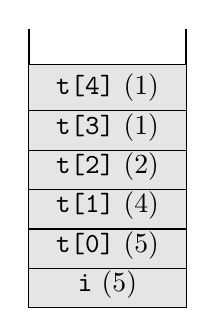
\begin{tikzpicture}
				\tikzstyle{Node} = [rectangle, minimum width=2cm, minimum height=5mm, text centered, draw=black, fill= gray!20]
				\tikzstyle{arrow} = [thick,->,>=stealth]
				
				\draw [thick, black] (0, 0) -- (2, 0);
				\draw [thick, black] (0, 0) -- (0, 3.5);
				\draw [thick, black] (2, 0) -- (2, 3.5);
				\node (c2) [Node] at (1,0.25) {\texttt{i} (5)};
				\node (d2) [Node] at (1,0.75) {\texttt{t[0]} (5)};
				\node (d2) [Node] at (1,1.25) {\texttt{t[1]} (4)};
				\node (d2) [Node] at (1,1.75) {\texttt{t[2]} (2)};
				\node (d2) [Node] at (1,2.25) {\texttt{t[3]} (1)};
				\node (d2) [Node] at (1,2.75) {\texttt{t[4]} (1)};
			\end{tikzpicture}
			\smallskip
			
			A \texttt{main} függvény változói.
		\end{figure}
		\subsection{Biztonsági rések nem definiált viselkedés következében}
		Irassuk ki a a tömb elemeit! (de ezt basszuk is el!)
		\begin{lstlisting}
for (int i = 0; i < 6; i++) //nem 6 elemes
{
	std::cout << t[i] << std::endl;
}
		\end{lstlisting} 
		Itt előre látható, hogy túl fogunk indexelni. Ez így egy {nem definiált viselkedés}hez vezet. Várhatóan valamilyen random memóriaszemetet fog kiolvasni (vagy olvashat ki, lévén nem definiált), és sose tudhatjuk pontosan mit.
		
		Most növeljük meg az elemeket, és menjünk el egészen 100ig!
		\begin{lstlisting}
for (int i = 0; i < 100; i++)
{
	++t[i];
}
std::cout << "sajt" << std::endl;
		\end{lstlisting} 
		Ez szintén nem definiált. Mivel olyan memóriaterületeket szeretnénk módosítani, melyeket nem foglaltunk le a programunknak, bajba juthatunk. Itt az órán a {sajt} szöveg ki lehet írva, mégis kaptunk szegmentálási hiba (\textit{segmentation fault}) hibaüzenetet az oprendszertől.
		
		\begin{lstlisting}
for (int i = 0; i < 100000; i++)
{
	++t[i];
}
std::cout << "sajt" << std::endl;
		\end{lstlisting} 
		Itt már (legalábbis ebben az esetben) előbb vágta magát hanyat a program, mielőtt sajt-ot ki tudta volna íratni. Ez jól demonstrálja, hogy ugyanazt  a hibát követtük el, de más volt a végeredmény. Ezért igazán veszélyesek a nem definiált viselkedések.
		\begin{lstlisting}
#include <iostream>
#include <string>

int main()
{
	int t[] = {5,4,3,2,1};
	int isAdmin = 0;
	std:string name;
	std::cin >> name;
	for (int i = 0; i < name.size(); ++i)
	{
		t[i] = 1;
	}
	if (name == "pityu")
		isAdmin = 1;
	std::cout << "Admin?: " << (isAdmin != 0 ) << std::endl;
}
		\end{lstlisting}
		Ha a programnak \texttt{pityu}-t adunk meg amikor be akarja olvasni \texttt{name}-et, akkor minden a legnagyobb rendben. De mivel a forráskódot ismerjük, azért hogyha nagyon hosszú nevet adnánk (nagyobb mint 5), akkor a túlindexelés miatt ki tudjuk használni a nem definiált viselkedéseket, és az is előfordulhat, hogy az \texttt{isAdmin} memóriacímére írunk, és elérjük hogy akkor is adminnak higgyen minket, ha nem vagyunk azok.
		\medskip
		
		Hogyan lehet ezeket a hibákat elkerülni? Túl azon, hogy nagyon figyelni kell, vannak programok amik segítenek nekünk. Ehhez használhatunk \texttt{sanitizer}-eket. Ezek picit módosítanak a kódunkon, és amennyiben futási időben bizonyos nem definiált viselkedéseket követne el, pl. itt a túlindexelés, leütné a programunkat. Használatukhoz elég egy extra paranccsal fordítanunk:
		
		{\centering\texttt{g++ main.cpp -fsanitize=address}\par }
		
		De sajnos ez is csak akkor tud segíteni, ha a probléma előfordul (azaz futási időben, nem fordítási időben ellenőriz). Amennyiben előfordul viszont, elég pontos leírást tudunk kapni arról, hogy merre van a probléma.
		
		{\centering \texttt{g++ main.cpp -Wall -Wextra} \par}
		
		Ez a 2 parancs szintén extra ellenőrzéseket vezet be, de nem változtatják meg a kódot, csak fordítási időben ellenőriznek.
	\subsection{Hivatkozás tömb elemeire}
		\begin{lstlisting}
#include <iostream>

int main()
{
	int t[] = {5,4,3,2,1};
	int *p = t;
	std::cout << *p << std::endl;
	std::cout << sizeof(int) << std::endl;
	std::cout << sizeof(p) << std::endl;
	std::cout << sizeof(t) << std::endl;
}
		\end{lstlisting}
		Könnyű azt hinni (hibásan) hogy a pointerek ugyanazok mint a tömbök. Ez  program jól mutatja, hogy ez nem igaz, mert a tömb tárolja annak méretét is. Számos más különbség is van, viszont egy tömb könnyen konvertálódik pointerré.
		
		Egy tömb adott elemét sokféleképpen le tudjuk kérdezni:
		
		{\centering \texttt{*(p + 3) == *(3 + p) == p[3] == 3[p]} \par}
		\
		\begin{lstlisting}
#include <iostream>

int main()
{
	int t[][3] = {{1,2,3},{4,5,6}};
	return 0;
}
		\end{lstlisting}
		Ez egy alternatív módja egy tömb inicializálásának. Itt több dolog megfigyelendő: Az első \texttt{[]} operátorban nincs méret, mert a fordító az inicializáció alapján meg tudja állapítani, hogy a mátrix azon dimenziója mekkora, de annyira már nem okos, hogy a másodikat is abszolválja.
		
		\medskip
		Fontos megjegyezni, hogy a mátrix egy adott elemére még többféleképpen tudunk hivatkozni:
		\medskip
		
		\begin{center}
			\texttt{t[1][] == *(*(t+1)+0) == *(1[t]+0) == 0[1[t]] == 0[*(t+1)] == *(t+1)[0] == 1[t][0] } 
		\end{center}
	\begin{note}
		Ahhoz, hogy egy olyan függvényt írjunk ami minden méretű tömböt elfogad paraméterül, a legegyszerűbb megoldás, ha hagyjuk, hogy a tömb átkonvertáljon egy olyan pointerré, ami az első elemre mutat, és átadjuk külön paraméterben a tömb méretét. Bár van megoldás arra is, hogy egy darab "rugalmas" függvényt írjunk, és az egész tömbhöz csak 1 paramétert vegyünk át, annak is komoly hátulütői lehetnek. Majd template-ekkel a 7-8. gyakorlaton lesz részletesen szó, de kb így nézne ki:
		\begin{lstlisting}
template <class T, int ArraySize>
void ( T (&param)[ArraySize] )
{
	//...
}
		\end{lstlisting}
		\smallskip
		Ez később jobban ki lesz fejtve, de itt egy template paraméter dedukció fog létrejönni, és a fordító kitalálja \texttt{param} méretét. Csak nyilván, mindig amikor egy más méretű tömböt hozunk létre, a fordító példányosítja ezt a függvényt, ami csúnyán meg tudja dobni a bináris kódot (\textit{binary code}).
		
		\smallskip
		A tömbök átvétele paraméterként azért ilyen körülményes, mert egy tömbnek a méretét fordítási időben ismernünk kell. Ha változó méretű tömböt várnánk paraméterül, az szembemenne ezzel a követelménnyel.  
	\end{note}
	\begin{note}
		Progalapon úgy tanultunk tömböket, hogy változó méretet adtunk meg nekik. Ezt a \texttt{gcc} compiler elfogadja, lefordítja, és jó kódot is csinál belőle, de nem garantált, hogy ezt minden fordító megteszi, ugyanis a c++ szabvány azt mondja ki, hogy a tömb méretének fordítási időben ismertnek kell lennie. Ez jól demonstrálja, hogy a compilerek nem feltételnül követik szorosan a szabványt.
	\end{note}
	\subsection{Tömbök átadása függvényparaméterként}
	Próbáljunk meg egy tömböt érték szerint átadni egy függvénynek!
	\begin{lstlisting}
#include <iostream>

void f(int t[])
{
	std::cout << sizeof(t) << std::endl;
}

int main()
{
	int t[] = {1,2,3,4,5};
	std::cout << sizeof(t) << std::endl;
	f(t);
}
	\end{lstlisting}
	Kimenet: \texttt{20 8} (ezen az implementáción)
	
	Bár mindkétszer azt hittünk hogy \texttt{t} tömb által foglalt méretét írattuk ki, és azt várnánk hogy a két szám ugyanaz lesz, a valóságban amikor azt érték szerint megpróbáljuk átadni, a \texttt{t} tömb átkonvertálódik a tömb elejére mutató pointerré.
	\begin{lstlisting}
void f(int t[8])
{
	std::cout << sizeof(t) << std::endl;
}
	\end{lstlisting}
	Ebben az esetben még mindig 8 lesz a második kiírt szám. Az a tanulság, hogy ha érték szerint akarunk átadni egy tömböt, ahelyett át fog konvertálódni pointerré. Az, hogy ezt szintaktikailag miért tehetjük meg mégis, hogy egy tömböt írunk oda mégis pointert kapunk, 
	\begin{center}
		\textit{,,az egy faszság.''}
		
		/Horváth Gábor/
	\end{center}
	\begin{note}
		Tömböt értékül adni a szabvány szerint nem is lehet: \texttt{int *t2[5] = t} nem helyes.
	\end{note}
	Korábban megismerkedtünk egy módszerrel, mely segítségével egy tömb méretét (elemszámát) paraméterátadás után is megőriztük:
	\begin{lstlisting}
#include <iostream>

void f(int *t, int size) //uj parameter!
{
	std::cout << sizeof(t) << std::endl;
}

int main()
{
	int t[] = {1,2,3,4,5};
	std::cout << sizeof(t) << std::endl;
	f(t, sizeof(t)/sizeof(t[0]));
}
	\end{lstlisting}
	\begin{note}
		Amennyiben c++11ben programozunk, érdemes az \texttt{std::array}-t használnunk, ami majdnem ugyanaz, mint egy tömb, legalább olyan hatékony, de nem tud pointerré változni és mindig tudja a méretét.
	\end{note}
	Ha szeretnénk egy tömböt egy darab paraméterrel átadni, megpróbálhatunk egy tömbre mutató pointert létrehozni. Azonban figyelni kell a szintaktikára, ha \texttt{int *t[5]}-t írunk, egy öt elemű intre mutató pointereket tároló tömböt kapunk.
	
	\medskip
	Ha valóban tömbre mutató mutatót szeretnék, így csinálhatjuk:
	\begin{lstlisting}
void g(int (*t)[5])
{
	std::cout << sizeof(t) << std::endl;
}
	\end{lstlisting}
	Azonban ez még mindig 8at fog kiírni (ezen az implementáción!), mert a \texttt{t} az egy sima mutató! Ahhoz, hogy megkapjuk, mire mutat, dereferálnunk kell, így a \texttt{sizeof} paraméterének \texttt{*t}-t kell megadni.
	\begin{note}
		Nyilván, ha refenreciával vennénk át \texttt{t}-t, az is hasonlóan nézne ki:\, \texttt{int (\&t)[5]}.
	\end{note}
	\medskip
	
	Ha megnöveljük a tömb méretét eggyel, akkor nem fordul le a kód, mert nem tud a g függvényben egy 5 elemű tömbre mutató mutató 6 elemű tömbre mutató mutatóvá konvertálódni.
	\begin{lstlisting}
int main()
{
	int a[6];
	g(a); //forditasi hiba!
	int b[5];
	g(b); //ok
}
	\end{lstlisting}
	
	\section{Literálok}
	\subsection{Karakterláncok}
	Mi lesz a \texttt{"Hello"} sztring típusa?
	\smallskip
	
	Egy konstans karakterekből álló 6 méretű tömb (\texttt{const char[6]}). Azért nem 5 elemű, mert a sztring el végén el kell tárolni a végét jelző \texttt{\textbackslash 0} karaktert.
	
	\begin{center}
		\begin{tabular}{|c|c|c|c|c|c|}
			\hline
			H&E&L&L&O&$\backslash$0\\
			\hline
		\end{tabular}
	\end{center}
	\begin{lstlisting}
int main()
{
	char* = "Hello";
}
	\end{lstlisting}
	A fenti kódban megsértettük a konstans korrektséget, hisz egy nem konstans pointerrel mutatuk egy konstans sztringre. Ennek ellenére, a fenti kód lefordul. Ez azért van, mert az eredeti C-ben nem volt konstans kulcsszó, és a kompatibilitás végett c++ban lehet konstans karaktertömbre nem konstans pointerrel mutatni.
	\begin{note}
		Ez egy nagyon rossz dolog, és kerülni kell, amennyire csak lehet. Lefordul, de kapunk rá warningot.
	\end{note}
	\begin{lstlisting}
int main()
{
	const char *hello = "Hello";
	hello[1] = o;
}
	\end{lstlisting}
	Ha eljászuk azt, hogy az egyik elemet o-ra cseréljük, akkor nem definiált viselkedést kapunk. 
	%TODO Sajnos ebből nem tudtam jobb leírást kipofozni tudáshiány végett.
	
	Futtatáskor (legalábbis ebben az esetben, hisz nem definiált viselkedésről van szó) futási idejű hibát kapunk, méghozzá szegmentálási hibát. Ennek a magyarázata a követekző: van a gépünknek sima és virtuális memóriája. Megfigyelhető, hogy sokkal több memóriát tudunk használni, mint amennyi ténylegesen van. Ez úgy oldható meg, hogy a virtuális memórián az alkalmazásunk kap egy memóriaterületet. Ezen a memóriacímen vannak olyan adatok is, melyek garantáltan nem változnak: a program kódja, és a fenti \texttt{"Hello"} szint is ilyen. Ezek külön vannak tárolva azok adatoktól, melyek változhatnak. 
	
	Ha ezt a programot mégegyszer elindítjuk, a memóriában kapni fog egy újabb színteret a program, amiben benne lesznek az adatok, melyeket futási időben módosíthat, illetve azok amiket nem. Az operációs rendszerünk azonban van olyan okos, hogy nem rakja be a nem módosítható adatokat még egyszer: a nem változtatható kódot a 2 külön működő azonos program ugyanarra a részére fogja irányítani a virtuális memóriában.
	
	\medskip
	Erre jó példa az, hogy a C-nek a standard könyvtárait közel minden program használja, így olcsóbb úgy megoldani, hogy minden programot ugyanide mutat.
	
	\medskip
	Miért kapunk szegmentálási hibát? A konstansok ezen nem módosítható részen belül vannak. Ha módosítanánk, akkor a másik program futása is változna. Az olyan programokat, amik ilyet próbálnak csinálni, szinte azonnal ki lesznek írtva. Az operációs rendszernek ugyanis nagyon fontos az, hogy a programok egymás futását nem zavarják (\textit{szeparálja} őket).
	
	\medskip
	Ez jól rámutat arra, hogy miért is nem jó az, ha a fenti hibát megengedjük.
	\subsection{Szám literálok} %TODO tuti jó ez a cím?
	Függően attól hogy egy számot hogyan írunk c++ban, mást jelenthet:
	\begin{center}
		\setlength{\extrarowheight}{2pt}
		\begin{tabular}{|c|l|}
			\hline
			\texttt{5}						&\texttt{int}\\
			\hline
			\texttt{5.}						&\texttt{double}\\
			\hline
			\texttt{5.f}					&\texttt{float}\\
			\hline
			\texttt{5e-4}					&\texttt{double}, értéke 0.0005\\
			\hline
			\texttt{5e-4f}					&\texttt{float}\\
			\hline
			\multirow{2}{*}{\texttt{0xFF}}	&{16-os számrendszerben}\\
											& ábrázolt \texttt{int}\\
			\hline
			\multirow{2}{*}{\texttt{012}}	&{8-as számrendszerben}\\
											&ábrázolt \texttt{int}\\
			\hline
			\texttt{5l}						&\texttt{long int}\\
			\hline
			\texttt{5u}						&\texttt{unsigned int}\\
			\hline
			\texttt{5ul}					&\texttt{unsigned long int}\\
			\hline
		\end{tabular}
		\end{center}
	\begin{note}
		Alapértelmezetten minden \texttt{int} egy \texttt{signed int}.
	\end{note}
	\begin{note}
		Viszonylag kevés esetben éri meg \texttt{float}-ot használni \texttt{double} helyett. Modern CPU-k ugyanolyan hatékonyan dolgoznak mind a kettővel, így érdemesebb a pontosabbat választani. (Ha magát a GPU-t programozzuk, az lehet egy kivétel.)
	\end{note}
	
	Létezik c++ban \texttt{signed} kulcsszó, mely eredetileg a char miatt volt, mert az is egész számokat tartalmazott, de azt nem definiálták külön, hogy a \texttt{char} lehessen vagy ne lehessen signed, ezért az, hogy egy adott platformon lehet-e az, az implementációfüggő.
	\begin{note}
		Érdemes mindig \texttt{int}et használnunk, hacsak nincs jó okunk arra, hogy \texttt{short}-ot, vagy \texttt{long}-ot írjunk. Az \texttt{int}-el általában a leghatékonyabb a processzor.
	\end{note}
	\section{Struktúrák mérete}
	A \texttt{sizeof(char)} mindig 1-et ad vissza. A karakter mérete mindig az egység. Minden más típusra a \texttt{sizeof} függvény azt adja vissza, hogy paraméterül megadott dolog mennyi \texttt{char} méretű. 
	
	A kérdésre, hogy mennyi \texttt{sizeof(char)}, a válasz mindig 1, de hogy ezt valóban hány byte-on tároljuk, az már implementációfüggő.
	
	\medskip
	A \texttt{char} méretén túl minden másnak a \texttt{sizeof}-ja teljesen implementációfüggő, bár a szabvány kimond pár szabályt:
	\begin{center}
		\texttt{sizeof(int) == sizeof(signed) == sizeof(unsigned)}
		\smallskip
		
		\texttt{sizeof(float) == sizeof(double) == sizeof(long double)}
		\smallskip
		
		\texttt{sizeof(short) $\leq$ sizeof(int) $\leq$ sizeof(long)}
		\smallskip
		
		\texttt{sizeof(char) == sizeof(unsigned char) == sizeof(signed char)}
		\smallskip
		
		\texttt{sizeof(char) $\leq$ sizeof(bool)}
		\smallskip
	\end{center}
	\begin{lstlisting}
#include <iostream>

struct Hallgato
{
	double atlag;
	int kor;
	int magassag;
}

int main()
{
	std::cout << sizeof(double) << std::endl;
	std::cout << sizeof(int) << std::endl;
	std::cout << sizeof(Hallgato) << std::endl;
}
	\end{lstlisting}
	Ezen a gépen a \texttt{double} mérete 8, az \texttt{int} mérete 4, \texttt{Hallgato}-é 16. Ezen azt látjuk, hogy a \texttt{Hallgato} tiszta adat.
	\begin{lstlisting}
struct Hallgato
{
	int kor;
	double atlag;
	int magassag;
}
	\end{lstlisting} 
	Amikor ennek a méretét kérdezzük le (figyeljük meg, hogy változott a sorrend), akkor a válasz már 24. Ennek az oka az, hogy míg az első esetben így volt eltárolva a memóriában: (ne feledjük, ez még mindig implementációfüggő!)
	\begin{figure}[H]
		\centering
		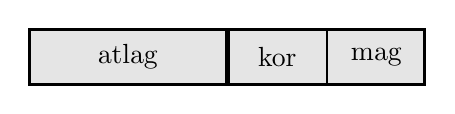
\begin{tikzpicture}
		\tikzstyle{Node} = [rectangle, minimum width=2.5cm, minimum height=7mm, text centered, draw=black, fill= gray!20, line width = 1.2pt]
		\tikzstyle{Border} = [rectangle, minimum width=2.5cm, minimum height=7mm, text centered, draw=black, line width = 1.2pt]
		\tikzstyle{HalfNode} = [rectangle, minimum width=1.25cm, minimum height=7mm, text centered, draw=black, fill= gray!20, line width = 0.2pt]
		\tikzstyle{arrow} = [thick,->,>=stealth]
		
		\node (1) [Node] {atlag};
		\node (2) [HalfNode, right = 0mm of 1] {kor};
		\node (3) [HalfNode, right = 0mm of 2] {mag};
		\node (border) [Border, right = -0.2mm of 1] {};
		
		\end{tikzpicture}
	\end{figure}
	Azaz, \texttt{atlag}, illetve \texttt{kor} és \texttt{magassag} pont efértek 1-1 gép szóban. Viszont, ha megcseréljük a sorrendet, ez már nem lesz igaz:
	\begin{figure}[H]
		\centering
		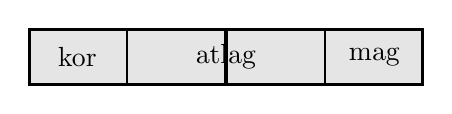
\begin{tikzpicture}
		\tikzstyle{Node} = [rectangle, minimum width=2.5cm, minimum height=7mm, text centered, draw=black, fill= gray!20]
		\tikzstyle{Border} = [rectangle, minimum width=2.5cm, minimum height=7mm, text centered, draw=black, line width = 1.2pt]
		\tikzstyle{HalfNode} = [rectangle, minimum width=1.25cm, minimum height=7mm, text centered, draw=black, fill= gray!20, line width = 0.2pt]
		\tikzstyle{arrow} = [thick,->,>=stealth]
		
		\node (1) [HalfNode] {kor};
		\node (2) [Node, right = 0mm of 1] {atlag};
		\node (3) [HalfNode, right = 0mm of 2] {mag};
		\node (border) [Border, right = -1.26cm of 1] {};
		\node (border) [Border, left = -1.26cm of 3] {};
		\end{tikzpicture}
	\end{figure}
	Sajnos itt már szétvágná \texttt{atlag}-ot. Ez nagyon nem hatékony, mert állandóan gondolnia kéne a fordítónak arra, hogy épp hogyan kaparja össze \texttt{atlag}-ot.
	\begin{figure}[H]
		\centering
		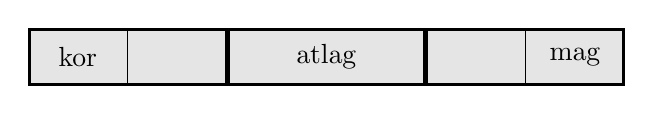
\begin{tikzpicture}
		\tikzstyle{Node} = [rectangle, minimum width=2.5cm, minimum height=7mm, text centered, draw=black, fill= gray!20, line width = 1.2pt]
		\tikzstyle{HalfNode} = [rectangle, minimum width=1.25cm, minimum height=7mm, text centered, draw=black, fill= gray!20, line width = 0.2pt]
		\tikzstyle{Border} = [rectangle, minimum width=2.5cm, minimum height=7mm, text centered, draw=black, line width = 1.2pt]
		\tikzstyle{arrow} = [thick,->,>=stealth]
		
		\node (1) [Node] {atlag};
		\node (2) [HalfNode, left = 0mm of 1] {};
		\node (3) [HalfNode, left = 0mm of 2] {kor};
		\node (4) [HalfNode, right = 0mm of 1] {};
		\node (5) [HalfNode, right = 0mm of 4] {mag};
		\node (border) [Border, right = -0.2mm of 1] {};
		\node (border) [Border, left = -0.2mm of 1] {};
		\end{tikzpicture}
	\end{figure}
	Ez így sokkal hatékonyabb, bár 3 gép szót használ. Ebben az esetben a kód eltárolja, hogy legyen egy kis \textit{padding } a változó után. Tehát semmi extráért nem kell fizetnünk, de attól még picit több memóriát foglalunk le.
	\smallskip
	
	A szabvány kimondja, hogy egy \texttt{struct} mérete az adottagok méreteinek összegénél nagyobbegyenlő.
	\smallskip
	
	Az, hogy egy gépi szó mekkora, implementációfüggő.
	\bigskip
	
	Egy \texttt{struct} egyes adattagjaira így hivatkozhatunk:
	\begin{lstlisting}
int main()
{
	//...
	Hallgato a;
	std::cout << a.kor << std::endl;
	Hallgato b = a;
	b.magassag = 3;
}
	\end{lstlisting}      
	
	\section{A c++ memóriamodellje}
	A c++ szabvány 3 memóriatípust különít el. Ezek közül főleg a stack-et használtuk eddig.
	\begin{center}
		\begin{tabular}{|c|}
			\\
			\\
			\\
			\\
			stack\\
			\\
			\hline
		\end{tabular}\quad 
		\begin{tabular}{|c|}
			\hline
			\quad \quad \\
			\\
			Globális/statikus\\
			\\
			\hline
		\end{tabular}\quad 
		\begin{tabular}{|c|}
			\hline
			\quad \quad \\
			\\
			Heap/free storage\\
			\\
			\hline
		\end{tabular}
	\end{center}
	\subsection{Stack}
	A második gyakorlaton már volt szó részletesebben a stack működéséről. Jusson eszünkbe egy nagyon fontos tulajdonsága: azok a változók, amelyekre már többet nem tudunk hivatkozni, automatikusan megsemmisülnek, így nem kell a létrehozással és a megsemmisítéssel külön bajlódnunk.
	\smallskip
	
	A stack-en létrehozott változókat szokás \textbf{automatikus változók}nak (\textit{automatic variable}) is hívni.
	
	\smallskip
	Vegyük példaként a második gyakorlatról már ismerős kódrészletet.
	
	\begin{lstlisting}
#include <iostream>

int f()
{
	int x = 0;
	++x;
	return x;
}

int main()
{
	std::cout << f() << std::endl;
	std::cout << f() << std::endl;
	std::cout << f() << std::endl;
	std::cout << f() << std::endl;
	std::cout << f() << std::endl;
}
	\end{lstlisting}
	Kimenet: \texttt{1 1 1 1 1}
	\smallskip
	
	A stacken lérehozott változók kezelése nagyon kényelmes, mert jól látható, mikor jönnek jönnek létre, mikor semmisülnek meg, stb. Azonban fordulhat elő olyan, hogy nem szeretnénk, hogy minden alkalommal megsemmisüljön a fenti példában az \texttt{x}, ilyenkor kiút lehet a statikus változók használata.
	\subsection{Globális/statikus tárhely}
	%TODO globális változók
	Írjuk át a fenti \texttt{f} függvényt, hogy \texttt{x} ne automatikus, hanem \textbf{statikus változó} (\textit{static variable}) legyen!
	\begin{lstlisting}
int f()
{
	static int x = 0;
	++x;
	return x;
}

int main() {/*...*/}
	\end{lstlisting}
	Kimenet: \texttt{1 2 3 4 5}
	
	Ebben az esetben azonban a függvény első hivásától a program futásának végéig benne marad a memóriában az \texttt{x}, így mindig egyre nagyobb számokat ad majd \texttt{f()} vissza.
	\begin{note}
		Nem igazán szeretjük a \texttt{static} változókat. Például a multithread programok különösen tudnak szenvedni tőle, mert nehéz, vagy lehetetlen átlátni, hogy mikor mire változik az értékük.
	\end{note}
	Amennyiben azt szeretnénk hogy \texttt{x} ne is semmisüljön meg azonnal, de statikus se legyen, létrehozhatjuk úgy, hogy a megsemmisítéséről is nekünk kell gondoskodni.
	\subsection{Heap/free storage}
	A heap-en létrehzoott változókat \textbf{dinamikus változók}nak (\textit{dynamic variable}) is szokás szokás hívni. A heap segítségével nagyon nagy szabadságra tehetünk szert, azonban ez a szabadság kötelességekkel is jár.
	\begin{lstlisting}
int main()
{
	int *p = new int(5);
	delete p;
}
	\end{lstlisting}
	Fentebb láthatjuk hogyan lehet egy változót a heap-en létrehozni. Ehhez használatos a \texttt{new} operátor, a heapen lefoglalandó memória típusa (ez esetben \texttt{int}), és konstruktor paraméterek (itt példaképp 5 kezdőértékkel inicializálink). Fontos, hogy a stack-et teljesen nem kerültük meg, mert szükségünk van egy pointerre, mely a heap-en kezelt címre mutat (\texttt{p}).
	
	Ezt a címet a \texttt{delete} operátorral tudjuk felszabadítani.
	\begin{figure}[!h]
		\centering
		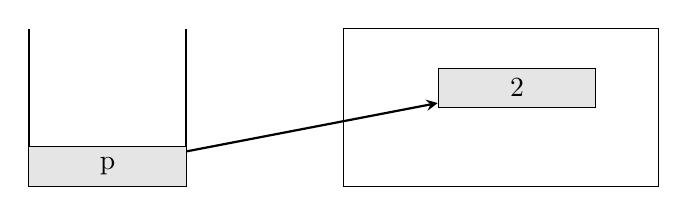
\begin{tikzpicture}
		\tikzstyle{Heap} = [rectangle, minimum width=4cm, minimum height=2cm, text centered, draw=black, fill=white]
		\tikzstyle{Stack} = [rectangle, minimum width=3cm, minimum height=1cm, text centered, draw=black, fill=white]
		\tikzstyle{ListNode} = [rectangle, minimum width=2cm, minimum height=5mm, text centered, draw=black, fill= gray!20]
		\tikzstyle{arrow} = [thick,->,>=stealth]
		
		%\foreach \x in {-2,-1,0,1,2,3,4}
		%	\draw (\x cm,1pt) -- (\x cm,-1pt) node[anchor=north] {$\x$};
		%\foreach \y in {-2,-1,0,1,2,3,4}
		%	\draw (1pt,\y cm) -- (-1pt,\y cm) node[anchor=east] {$\y$};
		%\draw[step=5mm,gray,very thin] (-2,-2) grid (6,6);
		
		\draw [thick, black] (-3, 0) -- (-1, 0);
		\draw [thick, black] (-3, 0) -- (-3, 2);
		\draw [thick, black] (-1, 0) -- (-1, 2);
		\node[Heap] at (3,1){};
		\node (2) [ListNode] at (3.2,1.25) {2};
		\node (p) [ListNode] at (-2,0.25) {p};
		\draw[arrow] (p) -- (2);
		\end{tikzpicture}
	\end{figure}
	
	A heapen nincs a változóknak nevük, így mindig szükségünk lesz egy mutatóra, hogy tudjunk rá hivatkozni. \textbf{Ha egyszer létrehozunk valamit a heap-en, nekünk is kell gondoskodni arról, hogy felszabadítsuk.} Az egyik leggyakoribb hiba a dinamikus memóriakezelésnél, ha a memóriát nem szabadítjuk fel, ilyenkor a lefoglalt memóriaterületre hivatkozni már nem lehet de lefoglalva marad, mondhatni elszivárog (\textit{memory leak}). 
	\smallskip
	
	Bár az operációs rendszer erre szokott figyelni, és megpróbál minden, a program által lefoglalt memóriát felszabadítani a dutás befejeztével, de nem mindenható, előfordulhat hogy ez nem elég teljeskörú, és ilyenkor az a memóriaterületek újraindításig lefoglalva maradnak.
	\medskip
	
	A dinamikus lefoglalt memória szabályos felszabadítását számos dolog nehezíti. Fényes példa erre a kivételkezelés, melynél hamarabb félbreszakítódik a függvény mintsem hogy felszabadítson minden memóriát. Azonban ha nagyon ügyelünk erre, előfordulhat hogy nem figyelünk, és egy memóriaterületet kétszer szabadítunk fel, ami nem definiált viselkedés.
	\medskip
	
	Előfordulhat, hogy egy már felszabadított memóriaterületre akarunk írni. Sajnos iylen hibát könnyű ejteni, hisz a \texttt{delete} a \texttt{p} által mutatott memóriaterületet, nem a \texttt{p}-t fogja törölni.
	\begin{note}
		A nullpointer törlésekor nem történik semmi (\textit{no-op}).
	\end{note}
	\begin{note}
		Amint elvesztettük az utolsó mutatót, ami egy adott lefoglalt memóriacímre mutat, az közel garantáltan elszivárgott memória. A szabvány nem foglal magában semmilyen lehetőséget ezeknek a visszaszerzésére (és könnyen látható, hogy ha meg is oldjuk, a szabványtól függetlenül hogy ezeket a memóriacímeket összevadásszuk, az igen költséges lenne).
	\end{note}
	Láthatjuk, hogy a heap használata macerás, hibaforrásokkal teli, ráadásul az allokálás (memória lefoglalás) még lassabb is. De miért használjuk mégis? Nos, ha egy mód van rá, ne tegyük. Ha meg lehet oldani, hogy a stack-en el tudjunk tárolni valamit, tegyük azt. A stacken azonban nem lehet mindent létrehozni, továbbá nagyon véges, hamar be tud telni (\textit{stack overflow}), illetve kevésbé tudjuk kontrollálni a memóriát. A heap-en e téren sokkal nagyobb a szabadságunk.
	\section{Osztályok felépítése}
	A következő pár gyakorlaton egy láncolt listát fogunk implementálni, mely jól demonstrálja majd a dinamikus memóriakezelés veszélyeit is.
	
	\smallskip
	A láncolt lista egy olyan konténer, melynek minden eleme egy olyan listaelem, mely tartalmaz egy mutatót és (legalább egy) adatot tároló objektumot. A listaelem mutatója rámutat a lista következő elemére, és az utolsó elem pointere pedig egy nullpointer.
	\begin{center}
		\begin{tabular}{|c|c|}
			\hline
			\texttt{data}&\texttt{*next}\\
			\hline
		\end{tabular}
		\smallskip
		
		Egy listaelem.
		\medskip
		
		\begin{tabular}{|c|c|}
			\hline
			\texttt{8}&\texttt{}\\
			\hline
		\end{tabular}$\rightarrow$
		\begin{tabular}{|c|c|}
			\hline
			\texttt{7}&\texttt{}\\
			\hline
		\end{tabular}$\rightarrow$
		\begin{tabular}{|c|c|}
			\hline
			\texttt{2}&\texttt{$\emptyset$}\\
			\hline
		\end{tabular}
		\smallskip
		
		3 elemű láncolt lista.
	\end{center}
	\subsection{Struct-ok}
	Egy láncolt lista elemét implementálhatjuk pl. így:
	\begin{lstlisting}
struct List
{
	int data;
	List *next;
};
	\end{lstlisting}
	Alkalmazzuk is ezt úgy, hogy  a listaelemek dinamikusan legyen eltárolva!
	\begin{lstlisting}
int main()
{
	List *head = new List;
	head->data = 8; //(*head).data   ==   head->data
	head->next = new List;
	
	head->next->data = 7;
	head->next->next = new List;
	
	head->next->next->data = 2;
	head->next->next->next = NULL;
	
	delete head;
	delete head->next;
	delete head->next->next;
}
	\end{lstlisting}
	Ezen a ponton mondhatjuk azt hogy készen vagyunk, hisz \texttt{List} használható láncolt listaként (bár valóban igen kényelmetlen).
	\medskip
	
	\begin{figure}[!h]
		\centering
		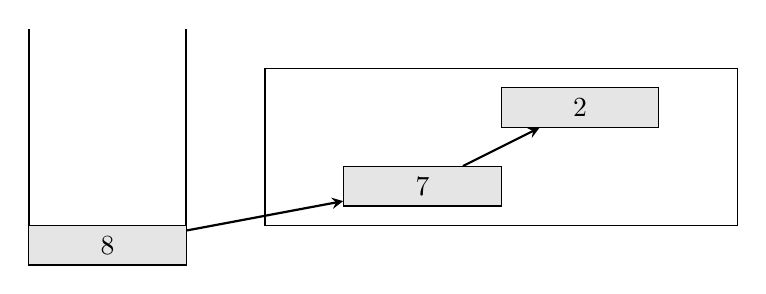
\begin{tikzpicture}
		\tikzstyle{Heap} = [rectangle, minimum width=6cm, minimum height=2cm, text centered, draw=black, fill=white]
		\tikzstyle{Stack} = [rectangle, minimum width=3cm, minimum height=1cm, text centered, draw=black, fill=white]
		\tikzstyle{ListNode} = [rectangle, minimum width=2cm, minimum height=5mm, text centered, draw=black, fill= gray!20]
		\tikzstyle{arrow} = [thick,->,>=stealth]
		
		%\foreach \x in {-2,-1,0,1,2,3,4}
		%	\draw (\x cm,1pt) -- (\x cm,-1pt) node[anchor=north] {$\x$};
		%\foreach \y in {-2,-1,0,1,2,3,4}
		%	\draw (1pt,\y cm) -- (-1pt,\y cm) node[anchor=east] {$\y$};
		%\draw[step=5mm,gray,very thin] (-2,-2) grid (6,6);
		
		\draw [thick, black] (-3, 0) -- (-1, 0);
		\draw [thick, black] (-3, 0) -- (-3, 3);
		\draw [thick, black] (-1, 0) -- (-1, 3);
		\node[Heap] at (3,1.5){};
		\node (7node) [ListNode] at (2,1) {7};
		\node (2node) [ListNode] at (4,2) {2};
		\node (headNode) [ListNode] at (-2,0.25) {8};
		\draw [arrow] (7node) -- (2node);
		\draw [arrow] (headNode) -- (7node);
		\end{tikzpicture}
	\end{figure}
	Sajnos a törlést sikerült picit elcsesznünk: először kitörljük a fejelemet (mely az első elemre mutat), viszont az első elem segítségével tudnánk a többi elemre is hivatkozni, így mire a második listaelemet törölnénk, \texttt{head} már egy felszabadított memóriaterületre mutat, amit törlés utáni használatnak (\textit{use after delete}) szokás nevezni, és az egy nem definiált viselkedés.
	
	A megoldás:
	\begin{lstlisting}
delete head->next->next;
delete head->next;
delete head;
	\end{lstlisting}
	\begin{note}
		A heap-en arra is figyelni kell, hogy jó sorrendben szabadítsuk fel a dolgokat. Könnyen lábonlőhetjük magunkat azzal, hogy egy kitörlünk valamit, ami hivatkozik egy másik memóriacímre, így azt a címet vagy elleakeljük, vagy ráhivatkozással nem definiált viselkedésbe keveredünk.
	\end{note}
	A változók a stacken fordított sorrendben semmisülnek meg, pont emiatt.
	\medskip
	
	Ez a ,,láncolt lista'' eddig eléggé gyér. A fő baj az, hogy nagyon sokat kell írni, méghozza lényegében ugyanazt, és nem feltétlenül kéne. Ez sért alap programozási gondolatmenetet, a DRY-t : \textit{Dont Repeat Yourself}. Itt sokszor írjuk le közel ugyanazt -- erre kell hogy legyen egy egyszerűbb megoldás. Írjunk függvényt az új listaelem létrehozásához!
	\begin{lstlisting}
List *add(List *head, int data)
{
	if (head == 0)
	{
		List *ret = new List;
		ret->data = data;
		ret->next = 0;
		return ret;
	}
	head->next = add(head->next, data);
	return head;
}
	\end{lstlisting}
	Ez egy olyan rekurzív függvény, mely addig hívja meg saját magát, míg a paraméterként kapott lista végére nem ér (azaz nem lesz \texttt{head} egy nullpointer). Amikor oda elér, létrehoz egy új listaelemet, ráfűzi a lista végére, és az új elem pointer adattagját (\texttt{next}) nullpointerré teszi.
	\medskip
	
	Nem ártana egy függvény a felszabadítsára is.
	\begin{lstlisting}
void free(List *head)
{
	if (head == 0)
		return;
	free(head->next);
	delete head;
}
	\end{lstlisting}
	Itt a rekurzió addig fog menni, amíg az utolsó elemhez el nem érünk, ami nullpointer. Itt simán visszatérünk, aztán fordított sorrendben kitörlünk minden elemet.
	\begin{note}
		A rekurzív függvények nem olyan hatékonyak, mint az iterativ (pl. \texttt{for} vagy \texttt{while} ciklus) társaik, továbbá a sok függvényhívás könnyen stack overflow-hoz vezetnek. Azonban jó agytornák, és segíthetnek az alapötletben. Egy rekurzív függvényt mindig át lehet írni iteratívvá.
	\end{note}
	Beszéljünk arról, mennyi a teher a felhasználón. Eddig tudnia kellett, milyen sorrendben kell felszabadítani midnent, de most már elég arra figylenie, hog lista használata után meg kell hívnia a \texttt{free} függvényt. A felhasználó így kisebb eséllyel követ el hibát, jobban tud figyelni arra, ami valóban a dolga. Legyenek a függvényeink és osztályaink olyanok, hogy \textbf{könnyű legyen őket jól használni, és nehéz legyen rosszul}.
	
	\subsection{Osztályra statikus változók}
	Teszteljünk!
	\begin{lstlisting}
int main()
{
	List *head = 0;
	head = add(head, 8);
	head = add(head, 7);
	head = add(head, 2);
	
	free(head);
}
	\end{lstlisting}
	A program lefordult, és (nálunk) tökéletesen le is futott. Azonban ha történt memory leak, az egy nem definiált viselkedés, így nem lehetünk benne biztosak, hogy valóban nem történt szivárgás. Egy lehetséges módszer, amivel megvizsgálhatjuk ezt, a statikus változók használata.
	
	\smallskip
	Az osztályon belül statikusként deklarált változókat osztályszintű változóknak is hívjuk, ugyanis minden, az osztályhoz tartozó objektum ugyanazon a statikus változón ,,osztozkodik''. Ha az egyiken keresztül azt a változót módosítjuk, a többiben módosulni fog. Élettartamuk és láthatóságuk a program elejétől végéig tart.
	
	Hozzunk létre \texttt{List}-ben egy számlálót, ami számon tartja mennyi objektumot hoztunk belőle létre, és semmisítettünk meg!
	\begin{lstlisting}
struct List
{
	int data;
	List *next;
	
	static int count; // !
};

List *add(List *head, int data)
{
	if (head == 0)
	{
		List *ret = new List;
		head->count++; // !
		ret->data = data;
		ret->next = 0;
		return ret;
	}
	head->next = add(head->next, data);
	return head;
}

void free(List *head)
{
	if (head == 0)
	return;
	free(head->next);
	head->count--; // !
	delete head;
}

int main()
{
	List *head = 0;
	head = add(head, 8);
	head = add(head, 7);
	head = add(head, 2);
	
	free(head);
	std::cout << head->count; // !
}
	\end{lstlisting}
	Azonban kaptunk egy fordítási hibát, miszerint hiányzik \texttt{count} definíciója -- Ahogy fent is említve volt, itt csak \textit{deklaráltuk}, de nem \texttt{definiáltuk} \texttt{count}-ot, így ezt tegyük is meg gyorsan.
	
	Osztályszintű változókat csak osztályon kívül tudunk definiálni (ezek alól kivételt képeznek az osztályszintű konstans változók):
	\begin{lstlisting}
int List::count;
	\end{lstlisting}
	Figyeljük meg, hogy \texttt{count}-nak nem adtunk kezdőértéket, hisz minden statikus változó (számok esetében) alapértelmezetten 0-ra incializál.
	\smallskip
	
	Mivel azonban ez a változó minden \texttt{List} objektummal közös, így nem muszáj egy változón keresztül hivatkozunk rá, a \texttt{List::count} kifejezéssel is megtehetjük.
	\medskip
	
	Ezzel a kis módosítással meg is kapjuk a kívánt kimenetet, \texttt{0}. Ez alapján tudhatjuk, hogy minden objektum törlésre került.
	\begin{note}
		A későbbiekben úgy tekintünk \texttt{List}-re, mintha ezeket a módosításokat nem ejtettük volna meg.
	\end{note}
	Ha azonban egy elemet kétszer töröltünk, az lehet, hogy nem derül ki. Ennek kiszűrésében segíthet, ha ezzel a paranccsal fordítjuk a kódunkat:
	\begin{center}
		\texttt{g++ list.cpp -fsanitize=address -g}
	\end{center}
	E segítségével úgy fordul a kód, hogy futási időjű ellenőrzéséket tesz bele a fordító, hogy nem szivárog-e a memória, vagy nem töröltük-e valamit kétszer (a \texttt{-g} a szebb hibaüzenetekhez kell). Ha ez bekövetkezne, megállítja a program futását, és ,,jól'' átlátható hibaüzenetet ad (bővebben: 3. gyakorlat anyaga). 
	
	\medskip
	Ez a láncolt lista még mindig messze áll egy jó struktúrától. Szerencsére nem csak adattagokat, de függvényeket is tudunk struct-okba írni, melyek alapértelmezetten hozzáférnek az adott objektum adattagjaihoz.
	\subsection{Konstruktorok}
	Próbáljuk megoldani azt, hogy ne kelljen egy listaelem adattagjainak mindig külön sorban értéket adni!
	\begin{lstlisting}
struct List
{
	List(int _data, List *_next = 0) : data(_data), next(_next) {}
	
	int data;
	List *next;
};
	\end{lstlisting}
	A fenti tagfüggvényt, vagy metódust \textbf{konstruktor}nak (\textit{constructor}, vagy röviden \textit{ctor}) hívjuk. A konstruktorok hozzák létre az objektumokat; vannak paraméterei, és nincs visszatérési értéke. A fenti konrtruktor még egy alapértelmezett paraméterrel is rendelkezik - ha mi csak egy \texttt{int} paraméterrel hívjuk meg a konstruktort, akkor a \texttt{\_next}-et alapértelmezetten nullpointernek veszi.
	
	\medskip
	Azonban a struktúránk működött eddig is, mégse írtunk konstruktort. Azonban az mindig kell a létrehozáshoz, hogyan lehet ez? Úgy, hogy a fordító a hiányzó kulcsfontosságú függvényeket megírja nekünk, létrehoz egy un. \textbf{default konstruktort} (többek között), ha mi explicit nem írtunk semmilyet, melynek nincsenek paraméterei, és minden adattagot alapértelmezetten hoz létre. Fontos azonban, hogyha mi írunk egy konstruktort, akkor a fordító már nem fog generálni ilyet.
	
	\medskip
	A kódban van továbbá egy un. \textbf{inicializációs lista}. Ez az a rész, ami a konstruktor paraméterei után kettőspont után következik. Az inicializációs lista elkerülhető néha, de nem éri meg általában. Ugyanis ha ezt írnánk:
	\begin{lstlisting}
List(int _data, List *_next = 0)
{
	data = _data;
	next = _next;
}
	\end{lstlisting}
	%TODO Ez szerintem nem igaz így.
	akkor mire a kapcsos zárójeles részhez érünk, addigra a \texttt{data} és a \texttt{next} létre lenne hozva, és utána kapna csak értéket. A fenti inicializációs listában az elemet a megadott értékkel inicializálódnak, és nem csak később kapnak értéket.
	\begin{note}
		A létrehozás és értékadás 2 lépés, az inicializálás csak 1.
	\end{note}
	Fontos megjegyzés, hogy az a struktúra elemei mindig megadott sorrendben inicializálódnak. Tehát, bármilyen sorrendben írjuk mi az inicializációs listát, mindig először a \texttt{data}, és utána a \texttt{next} fog inicializálódni, hacsak nem cseréljük fel a sorrendjüket a struct-ban.
	\subsection{Destrukorok}
	Ahogy gondoskodtunk a listaelemek létrehozásáról, gondoskodhatnánk annak megfelelő megsmmisüléséről is.
	\begin{lstlisting}
struct List
{
	//ctor (construktor)
	List(int data, List *next = 0) : data(data), next(next) {}
	//dtor (destructor)
	~List()
	{
		delete next;
	}
	
	int data;
	List *next;
};
	\end{lstlisting}
	Az fenti tagfüggvényt, melynél a hullámvonalat közvetlenül a struktúra neve követi \textbf{destruktor}nak (\textit{destruktor}, röviden \textit{dtor}) nevezzük. A destruktor mindig az objektum élettartamának végén hívódik meg, és gondoskodik az adattagok megsemmisítéséről. Lévén az élettartam végén hívódik meg ez a függvény, lehetőséget teremt nekünk arra, hogy a dinamikusan lefoglalt memóriacímeket felszabadítsuk.
	
	\medskip
	Ez is egy rekurzív függvény: a \textbf{next} törlésekor megpróbál kitörölni egy \texttt{List} típusú elemet, ami megint meghívja ezt a destruktort, stb. A lista végén a \texttt{next} egy nullpointer, azzal nem tesz semmit, a destuktor futása befejeződik, és fordított irányban kitöröl mindent.
	
	\medskip
	Teszteljünk!
	\begin{lstlisting}
int main()
{
	List head(8);
	add(&head, 7);
	add(&head, 2);
}
	\end{lstlisting}
	Most úgy alakítottuk át a kódot, hogy amikor létrehozzuk a listát, akkor a fejelemet a stacken hozzuk létre, melynek értéke 8, és a pointer része nullpointer. Később az \texttt{add} függvénnyel létrehozunk a heapen egy olyan listaelemet, mely 7-et tárol, és pointer része nullpointer, és az eredeti lista fejét ráállítjuk erre.
	\medskip
	
	Itt sikeresen elértük azt, hogy a lista első eleme a stack-en, de minden más eleme a heap-en legyen. Mivel olyan struktrát írtunk, mely gondoskodik arról, hogy minden dinamikusan lefoglalt területet felszabadítson, mindent csak egyszer töröl, jó sorrendben, egy  \textit{RAII} (\textit{Resource acquisition is initialization}) osztályt írtunk. Ez Bjorne-nek egy
	\begin{center}
		\textit{,,iszonyatosan szar''}
		
		/Horváth Gábor/
	\end{center}
	acronymje. Azt mondja ki, hogy a nyelv által garantált módon pontosan tudjuk hogy az objektumok mikor jönnek létre, mikor semmisülnek meg, stb.
	
	Bjorne továbbá kijelentette, hogy a c++ legjobban garbage kollektált nyelv, mert nincs benne garbage. Ha jól programozunk, akkor az objektumok mindig eltakarítanak maguk után. 
	\medskip
	
	Sikerült azt is elérnünk, hogy ez nagyon hatékony legyen, hiszen a ha nem így konstruktor/destruktor trükközéssel dogloznánk, akkor kézzel kéne írni, ami ennél nem lenne gyorsabb, csak kényelmetlenebb.
	
	\medskip
	Csináljunk az \texttt{add} függvényből metódust!
	\begin{lstlisting}
struct List
{
	List(int data, List *next = 0) : data(data), next(next) {}
	~List()
	{
		delete next;
	}
	
	
	void add(int data) //eltunt egy parameter!
	{
		if (next == 0)
		{
			next = new List(data);
		}
		else
		{
			next->add(data);
		}
	}
	int data;
	List *next;
};

int main()
{
	List head(8);
	head.add(7);
	head.add(2);
}
	\end{lstlisting}
	Ez a nyelv egyik szépsége, hisz a felhasználónak nem kell tudnia, mi megy a háttérben, sőt, még értenie se kell, mi történik a belső implementációban.
	\medskip
	
	\subsection{Másoló konstruktor}
	
	A fordító nagyon sokmindent megír a structunkba: konstruktoron és destruktoron kívül még \textbf{másoló konstruktor}t (\textit{copy constructor}) is ír. A másoló konstruktor egy olyan konstrukor, melynek egyetlen paramétere egy azonos típusú objektum. Azonban ez alapértelmezetten bitről bitre másol Ez mit jelent?
	\begin{lstlisting}
int main()
{
	List head(8);
	head.add(7);
	head.add(2);
	{
		List cHead = head;
	} //itt lefut cHead destruktora
}
	\end{lstlisting}
	Fentebb létrehoztunk egy új listát \texttt{head} mintájára. Nyilván, a másolatnak a destruktora hamarabb lefut. Futtatáskor (ha sanitizerrel fordítunk) egy kilométer hibaüzenetet kapunk: többször próbáltuk meg ugyanazt a memóriaterületet felszabadítani. Ennek az az oka, hogy a \texttt{cHead}-ben lévő pointer \textbf{ugyanarra} a listára fog mutatni (lévén a bitről bitre történő másolásnál a pointerek ugyanazt a memóriacímet adják értékül egymásnak), és a \texttt{cHead} megsemmisülése után a \texttt{head} is megpróbálja a már kitörölt listát kitörölni.
	
	%\resizebox{\textwidth}{!}{%
	\begin{figure}[!h]
		\centering
		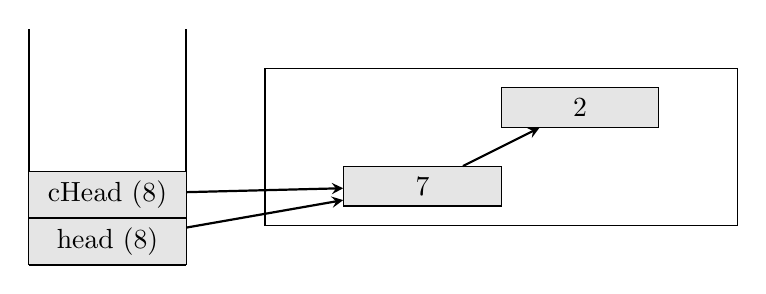
\begin{tikzpicture}
			\tikzstyle{Heap} = [rectangle, minimum width=6cm, minimum height=2cm, text centered, draw=black, fill=white]
			\tikzstyle{Stack} = [rectangle, minimum width=3cm, minimum height=1cm, text centered, draw=black, fill=white]
			\tikzstyle{ListNode} = [rectangle, minimum width=2cm, minimum height=5mm, text centered, draw=black, fill= gray!20]
			\tikzstyle{arrow} = [thick,->,>=stealth]
			
			%\foreach \x in {-2,-1,0,1,2,3,4}
			%	\draw (\x cm,1pt) -- (\x cm,-1pt) node[anchor=north] {$\x$};
			%\foreach \y in {-2,-1,0,1,2,3,4}
			%	\draw (1pt,\y cm) -- (-1pt,\y cm) node[anchor=east] {$\y$};
			%\draw[step=5mm,gray,very thin] (-2,-2) grid (6,6);
			
			\draw [thick, black] (-3, 0) -- (-1, 0);
			\draw [thick, black] (-3, 0) -- (-3, 3);
			\draw [thick, black] (-1, 0) -- (-1, 3);
			\node[Heap] at (3,1.5){};
			\node (7node) [ListNode] at (2,1) {7};
			\node (2node) [ListNode] at (4,2) {2};
			\node (cHeadNode) [ListNode] at (-2,0.9) {cHead (8)};
			\node (headNode) [ListNode] at (-2,0.3) {head (8)};
			\draw [arrow] (7node) -- (2node);
			\draw [arrow] (headNode) -- (7node);
			\draw [arrow] (cHeadNode) -- (7node);
		\end{tikzpicture}
		\smallskip
		
		Zárójelben a lista első elemének \texttt{data} adattagjának értéke.
	\end{figure}
	%}
	
	Kerüljük ki a hibát, és írjunk saját copy konstruktort!
	
	
\begin{lstlisting}
struct List
{
	//...
	
	List(const List &other) : data(other.data), next(0)
	{
		if (other.next != 0)
		{
			next = new List(*other.next);
		}
	}
	
	//...
};

int main()
{
	List head(8);
	head.add(7);
	head.add(2);
	{
		List cHead = head;
	}
}
\end{lstlisting}
	Mint a korábbi függvényeink, ez is rekurzióval működik: a \texttt{new List(*other.next)} újra és újra meghívja a copy konstruktort, amíg az other.next nem lesz nullpointer.
	\begin{figure}[!h]
		\centering
		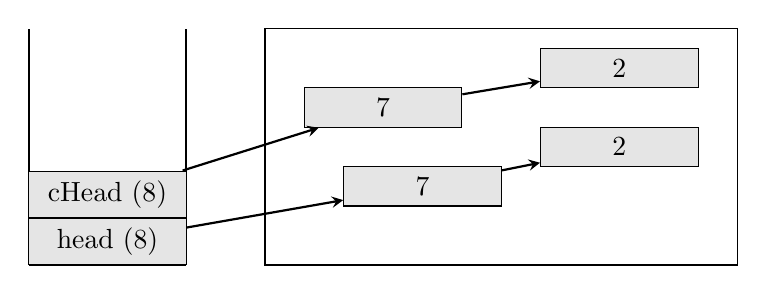
\begin{tikzpicture}
		\tikzstyle{Heap} = [rectangle, minimum width=6cm, minimum height=3cm, text centered, draw=black, fill=white]
		\tikzstyle{Stack} = [rectangle, minimum width=3cm, minimum height=1cm, text centered, draw=black, fill=white]
		\tikzstyle{ListNode} = [rectangle, minimum width=2cm, minimum height=5mm, text centered, draw=black, fill= gray!20]
		\tikzstyle{arrow} = [thick,->,>=stealth]
		
		%\foreach \x in {-2,-1,0,1,2,3,4}
		%	\draw (\x cm,1pt) -- (\x cm,-1pt) node[anchor=north] {$\x$};
		%\foreach \y in {-2,-1,0,1,2,3,4}
		%	\draw (1pt,\y cm) -- (-1pt,\y cm) node[anchor=east] {$\y$};
		%\draw[step=5mm,gray,very thin] (-2,-2) grid (6,6);
		
		\draw [thick, black] (-3, 0) -- (-1, 0);
		\draw [thick, black] (-3, 0) -- (-3, 3);
		\draw [thick, black] (-1, 0) -- (-1, 3);
		\node[Heap] at (3,1.5){};
		\node (7node) [ListNode] at (2,1) {7};
		\node (2node) [ListNode] at (4.5,1.5) {2};
		\node (7node2) [ListNode] at (1.5,2) {7};
		\node (2node2) [ListNode] at (4.5,2.5) {2};
		\node (cHeadNode) [ListNode] at (-2,0.9) {cHead (8)};
		\node (headNode) [ListNode] at (-2,0.3) {head (8)};
		\draw [arrow] (7node) -- (2node);
		\draw [arrow] (7node2) -- (2node2);
		\draw [arrow] (headNode) -- (7node);
		\draw [arrow] (cHeadNode) -- (7node2);
		\end{tikzpicture}
	\end{figure}
	
	\medskip
	Ezzel meg is oldottuk a problémát. 
	
	Figyelem, ez egy \textbf{copy konstruktor, nem értékadás operátor!} Itt a \texttt{cHead} még nincs létrehozva, amikor head-el \textbf{inicializálni} próbáljuk. Ha az egyenlőségjel bal oldalán lévő objektum még nem jött létre, mint itt, akor a copy konstruktor hívódik meg. Ellenkező esetben értékadás operátor.
	\begin{lstlisting}
List cHead = head; //copy ctor

List cHead;
cHead = head; //ertekadas
	\end{lstlisting}
	
	\subsection{Értékadó operátor}
	Másoló konstruktorunk már van, de az értékadással még mindig lábon lőhetjük magunkat. Hasonlóan a default másoló konstruktorhoz, alapértelmezetten az értékadás operátor (\textit{assignment operator}, vagy röviden \texttt{=}) is bitről bitre másol, így jobb ha felülírjuk.
\begin{lstlisting}
struct List
{
	//...
	
	//copy constructor
	List(const List &other) : data(other.data), next(0)
	{
		if (other.next != 0)
		{
			next = new List(*other.next);
		}
	}
	
	//assignment operator
	List& operator=(const List &other)
	{
		delete next;
		if (other.next) // if(other.next) == if(other.next != 0)
		{
			next = new List(*other.next);
		}
		else
		{
			next = 0;
		}
		return *this;
	}
	
	//...
};
\end{lstlisting}
	Az új értékadás operátorunk először kitörli az aktuális lista elemeit, majd rekurzív módon átmásolja \texttt{other} elemeit az aktuális listába.
	
	Példaképp, a legelső lépés a \texttt{delete next;}-el az összes aktuális listaelem felszabadítása, majd addig hívjuk meg az értékadást rekurzívan, míg az \texttt{other} lista végére nem érünk (erre van az \texttt{if} ág), és ha elértünk oda, akkor zárjuk le az aktuális listát egy nullpointerrel. 
	
	Sikerült elérnünk, hogy ha lemásoljuk a listát, és a másolatot módosítjuk, az eredeti lista nem fog változni.
	\medskip
	
	Figyeljök meg, hogy referenciával tértünk vissza. Ennek oka az, hogy meg tukjuk tenni ezt:
	\begin{lstlisting}
			int a = b = c = d = 0; // a = (b = (c = (d = 0)))
	\end{lstlisting}
	Itt rendre \texttt{d}-t, \texttt{c}-t, \texttt{b}-t, \texttt{a}-t adjuk vissza, így egymásba fűzhetjük az értékadást.
	\begin{note}
		Miért nem konstans referenciával térünk vissza? Azért, mert nem tehetnénk meg ezt: (legyen \texttt{f} egy nem konstanst váró függvény) \texttt{f(a = 0)}.
	\end{note}
	
	Írjunk egy egyszerűbb kiíratást is!
	\begin{lstlisting}
struct List
{
	//...
	
	void print ()
	{
		std::cout << data << ' ';
		if (next)
			next->print();
	}
	
	//...
};
	\end{lstlisting}
	Nézzük meg mit műveltünk!
	\begin{lstlisting}
int main ()
{
	List head(7);
	head.add(8);
	head.add(2);
	{
		List cHead = head;
	}
	head.print();
}
	\end{lstlisting}
	Kimenet: \texttt{7 8 2}
	
	Azonban itt még mindig van egy nagy veszély. Ha a listát saját magának adjuk értékül, akkor a legelső lépés továbbra is az, hogy kitöröljük az aktuális lista elemét. így \texttt{cHead = cHead} megsemmisíti önmagát, és use-after-free hibát követnénk el, amikor a destruktor lefut. Persze mondhatnánk, hogy ki az a hülye, aki ilyen csinálna, de sajnos ezt a hibát könnyebb elkövetni mint gondolnánk.
	\begin{lstlisting}
void f(List &l1, List &l2)
{
	//...
	l1 = l2;
	//...
}
	\end{lstlisting}
	Ha valaki ugyanazt a listát adja meg mindkét paraméternek, akkor máris megvan a baj. Módosítsuk az értékadás operátorunkat:
\begin{lstlisting}
List& operator=(const List &other)
{
	if (this == &other) return *this;
	delete next;
	if (other.next)
	{
		next = new List(*other.next);
	}
	else
	{
		next = 0;
	}
	return *this;
}
\end{lstlisting}
	Ezzel a probléma el is lett kerülve. Újdonság lehet a \texttt{this} kulcssszó -- ennek segítségével tudunk rámutatni tagfüggvényen belül az adott objektumra. Segíthet a megértésben, ha úgy tekintünk rá, hogy \texttt{head.print()} esetében például sehogyse tudnánk \texttt{print()}-en belül \texttt{head}-re hivatkozni, hisz az objektum neve tagfüggvényen belül nem elérhető. Ezt a problémát hivatott a \texttt{this} kulcsszó orvosolni. \texttt{this} egy konstans pointer, mely az objektum címére mutat.
	\medskip

	Sikeresen létrehoztunk egy \textit{reguláris típust}.
	\medskip
	
	Egy \texttt{T} típus \textbf{reguláris típus}, ha van neki:
	\begin{enumerate}
		\item konstruktora
		\item destruktora
		\item értékadás operátora, továbbá
		\begin{lstlisting}
T b;
T a;
a = b;
		\end{lstlisting}
		Ekkor \texttt{a} ekvivalens \texttt{b}-vel, és ha \texttt{a}-t módosítjuk, akkot \texttt{b} nem változik, és viszont.
		\item másoló konstruktora, továbbá
		\begin{lstlisting}
T b;
T a = b;
		\end{lstlisting}
		Ekkor \texttt{a} ekvivalens \texttt{b}-vel, és ha \texttt{a}-t módosítjuk, akkot \texttt{b} nem változik, és viszont.
		\item egyenlőségvizsgálat (\texttt{operator==}) (nem feltétlenül szükséges)
	\end{enumerate}
	\subsection{Adattagok védettsége}
	Már majdnem készen vagyunk, ám a hülye felhasználó még mindig lábon lőheti magát, pl így:
	\begin{lstlisting}
int main()
{
	List head(8);
	head.add(7);
	head.add(2);
	head.next = 0;
}
	\end{lstlisting}
	Itt az első listaelem utáni elemeket lecsatoljuk, és azoknak a memóriája elszivárog. A baj probléma az, hogy a \textbf{felhasználó hozzáfér az adattagokhoz.} A felhasználó így nagy hülyeséget csinálhat, továbbá ha gyakran hivatkozik belső adattagokra, egyéb baja is lehet. Példaképp, ha a \texttt{List} \texttt{next} adattagjának új nevet adunk, akkor át kéne írni minden olyan kódot ami \texttt{next}re hivatkozik.
	
	Jó lenne, ha hiába változna a belső reprezentáció, a kódnak nem kéne változnia. 
	
	Írjuk át ezt úgy, hogy a felhasználó ne férjen hozzá az adattagokhoz!

\begin{lstlisting}
class List //nem struct!
{
public:
	List(int data, List *next = 0) : //...
	void add(int data) {//...}
	List(const List &other) //...
	List& operator=(const List &other) {//...}
private:
	int data;
	List *next;
};
\end{lstlisting}
	Az osztály minden adattagja, metódusa mely a \texttt{public} kulcsszó után jön, elérhető bárki számára. A \texttt{private} kulcsszó után következő adatok csak is kizárólag az adott osztályon belül érhető el (nemsokára megismerkedünk egy kivétellel).

	A \texttt{class} majdnem ugynaz mint a \texttt{struct}, csak alapértelmezetten a \texttt{struct} minden adattagja és tagfüggvénye publikus, míg \texttt{class}-nak alapértelmezetten privát. A \texttt{public} ill. \texttt{private} kulcsszóval mind a kettőnél szabályozhatjuk a privát és publikust részt.
	
	\medskip
	Azonban van egy igen nagy probléma, ami ennek a módosításnak a követekzménye lett. Például az, hogy így sose tudunk hozzáférni a második elemhez kívülről. Vagy bármelyik másikhoz. Ilyenkor megoldás lehet az, ha módosítjuk a listát, és minden olyan függvényt,  aminek hozzá kéne férnie az elemekhez, metódussá tesszük, hisz a lista metódusai hozzáférnek a privát adattagokhoz is.
	
	Najó, ezt minden egyes függvénnyel lehet nem akarjuk megtenni. A végén egy kilóméter implementációnk lenne, ami nagyon rontaná az olvashatóságot.
	
	Írjunk felsorolót erre a célra, és utána meglátjuk hogy
	\begin{center}
		\textit{,,az úgy hülyeség ahogy van.''}
		
		/Horváth Gábor/
	\end{center}
\begin{lstlisting}
class List
{
	//...
	
	void First()
	{
		cursor = this;
	}
	int& Current()
	{
		return cursor->data;
	}
	void Next()
	{
		cursor = cursor->next;
	}	
	bool End()
	{
		return cursor == 0;
	}
	
private:
	int data;
	List *next;
	List *cursor;
};
\end{lstlisting}
	Figyeljük meg, hogy \texttt{Current()} referenciával tér vissza, hogy ne \texttt{data} másolatát, hanem magát a \texttt{data}-t kapjuk meg, így tudjuk a lista értékét módosítani.
	
	\medskip
	Első látásra a problémát orvosoltuk, tudunk a listákkal tárolt adatokkal dolgozni (pl. összeadni őket, stb). De egy rendezésnél már bajban lehetünk. Például csak 1 darab kurzorunk van, így nem tudunk egyszerre 2 elemhez hozzáférni, hogy összehasonlítsuk őket, lévén csak egy \texttt{cursor} van. Megoldás!:
\begin{lstlisting}
class List
{
	//...
	
	void First()
	{
		cursor = this;
	}
	int& Current()
	{
		return cursor->data;
	}
	void Next()
	{
		cursor = cursor->next;
	}	
	bool End()
	{
		return cursor == 0;
	}
	
	void First2()
	{
		cursor2 = this;
	}
	int& Current2()
	{
		return cursor2->data;
	}
	void Next2()
	{
		cursor2 = cursor2->next;
	}	
	bool End2()
	{
		return cursor2 == 0;
	}
	
private:
	int data;
	List *next;
	List *cursor;
	List *cursor2;
};
\end{lstlisting}
	Oké, ez viccnek talán jó, de könnyű látni, ha mondjuk 3 darab \texttt{cursor} kéne, akkor bajba lennénk, és hosszútávon nem ez a jó hozzáállás. Ez nem elég ahhoz, hogy komplex feladatokat meg tudjunk írni. \textbf{Munkahelyen ilyet ne írjunk!} Töröljük is ki gyorsan, és írjunk egy iterátort!
	\subsection{Iterátorok.}
	Az iterátorok a pointerek általánosítása, segítségükel tudunk végigiterálni egy konténer elemein (azaz velük tudjuk lekérdezni a konténer elemeit). Ehhez szükségünk van arra, hogy tudjuk hol kezdődik és végződik a konténerünk. E láncolt lista esetében hozzá tudunk férni az első elemhez (az lesz ugye \texttt{head} a fenti példákban) és tudjuk hogy mindig nullpointerrel végződik. Legyen az iterátunk neve \texttt{Iterator}!
\begin{lstlisting}
class List
{
	//...
public:
	Iterator begin()
	{
		return Iterator(this);
	}
	Iterator end()
	{
		return Iterator(0);
	}
};
\end{lstlisting}
	E két metódus segítségével már meg tudjuk adni a lista elejét és végét! \texttt{head.begin()} lesz \texttt{head} a legelső eleme, \texttt{head.end()} az utolsó utáni elem. Már csak magát az iterátort kell megírni, mely egy un. \textit{forward iterator} lesz.
	\medskip

	Egy \texttt{T} típus \textbf{forward iterator}, ha rendelkezik:
	\begin{enumerate}
		\item \texttt{++} operátorral
		\item egyenlőség vizsgáló operátorral \texttt{==}
		\item egyenlőtlenség vizsgáló operátorral \texttt{!=}
		\item dereferáló operátorral \texttt{*}
	\end{enumerate}
	De hova írjuk az \texttt{Iterator} osztályt? Hiszen ha a lista elé tesszük, az \texttt{Iterator} nem fogja tudni, hogy mi az a \texttt{List}. Ha utána tesszük, nem fogja tudni a \texttt{List} hogy mi az az \texttt{Iterator}, úgy meg nem műküdne az \texttt{end} és a \texttt{begin} metódus. Ehhez \textbf{forward deklarálni} fogunk.
	\begin{lstlisting}
class List; //forward declaration

class Iterator
{
public:
	Iterator(List *_p) : p(_p) {}
	bool operator==(Iterator &other)
	{
		return p == other.p;
	}
	bool operator!=(Iterator &other)
	{
		return !(*this == other);
	}
	//...
private:
	List *p; //(*)
};

class List {//...};
	\end{lstlisting}
	A fordító már a csillagozott sornál nem fog problémázni, hogy nem tudja mi az a \texttt{List} - arra számít hogy valamikor (akár egy másik fordítási egységben) \texttt{List} definiálva lesz. Amennyiben nem akarjuk dereferálni \texttt{p}-t, elég csupán a forward deklarálni, ki sem kell fejtenünk az osztály bővebben később!
	
	\medskip
	Még hiányzik a \texttt{++} és a \texttt{*} operátorunk.
\begin{lstlisting}
class List;

class Iterator
{
public:
	Iterator(List *_p) : p(_p) {}
	bool operator==(Iterator &other)
	{
		return p == other.p;
	}
	bool operator!=(Iterator &other)
	{
		return !(*this == other);
	}
	Iterator operator++()
	{
		p = p->next;
		return *this;
	}
	int& operator*()
	{
		return p->data;
	}
private:
	List *p;
};

class List {//...};
\end{lstlisting}
%TODO operator++ miért nem referenciával tér vissza?
	És itt az előbb említett problémába bele is ütköztünk: a fordító siránkozik, hogy a \texttt{List} egy un. \textit{incomplete type}. Ugyanis az tudja hogy van osztály hogy \texttt{List}, de az, hogy \texttt{next} adattag, nem tudja micsoda. Ezért ezeket a tagfüggvényeket a lista után kell írni.
\begin{lstlisting}
class List;

class Iterator
{
public:
	Iterator(List *_p) : p(_p) {}
	bool operator==(Iterator &other)
	{
		return p == other.p;
	}
	bool operator!=(Iterator &other)
	{
		return !(*this == other);
	}
	Iterator operator++();
	int& operator*();
private:
	List *p;
};

class List {//...};

Iterator Iterator::operator++()
{
	p = p->next;
	return *this;
}
int& Iterator::operator*()
{
	return p->data;
}
\end{lstlisting}
	Itt még mindig hisztizni fog a fordító: \texttt{next} és \texttt{data} annyira private, hogy még az \texttt{Iterator} se fér hozzá! Erre megoldás, hogyha \textbf{barát} (\textit{friend}) osztállyá tesszük.
	\begin{lstlisting}
class List
{
	//...
	friend class Iterator;
	//...
}
	\end{lstlisting}
	A barátként deklarált osztályok és függvények hozzá tudnak férni az osztály privát adattagjaihoz is.
	
	\smallskip
	Az így kapott iterátorunkkal végig tudunk menni a lista elemein, hozzá tudunk férni az adattagjaihoz. Így már azt is megtehetjük, hogy \texttt{print()}-et tagfüggvény helyett sima globális függvénnyé tesszük.
	\begin{lstlisting}
void print(List &l)
{
	for(Iterator it = l.begin(); it != begin(); ++it)
	{
		std::cout << *i << ' ';
	}
	std::cout << std::endl;
}
	\end{lstlisting}
	Ez a függvény, csak úgy mint az \textit{STL} függvények is (majd lesz még boncolgatva az, hogy mi az az \textit{STL}), balról zárt, jobbról nyitott $[\ )$ intervallummal dolgoznak. Azaz az \texttt{end()} már nem eleme a listának, az az utolsó \textit{utáni} elem (\texttt{past-the-end iterator}).
	
	\medskip
	Megint nyertünk! Annyi \texttt{Iterator}-t hozunk létre, amennyit csak akarunk, nem vagyunk korlátozva egy darab \texttt{cursor} által. Továbbá, elég azt írni, hogy \texttt{.begin(), .end()}, nem kell tudnunk, mi van az implementáció mélyén, \textbf{sőt}, a belső implementáció változhat is, akkor se lesz baj. Két programozó így teljesen jól együtt tud dolgozni.
	
	\medskip
	Megfigyelhető, hogy \texttt{print} nem módosítja a paraméterként kapott listát, így átvehetnénk konstansként is. Ennek az eredménye egy kilóméter fordítási hiba: amit az \texttt{end} és \texttt{begin} visszaad, nem konstans, azaz ezeken keresztül tudjuk módosítani az objektumot. Valahogy törekednünk kéne arra, hogy a konstans korrektséget betartsuk.
	\subsection{Konstans iterátorok}
	Erre a megoldás, ha konstans iterátort írunk, ami egy konstansra mutató mutató általánosítása.
\begin{lstlisting}
class List;

class Iterator
{
	//...
};

class ConstIterator
{
public:
	Const Iterator(const List *_p) : p(_p) {}
	bool operator==(ConstIterator &other) const //a metodus konstans!
	{
		return p == other.p;
	}
	bool operator!=(ConstIterator &other) const
	{
		return !(*this == other);
	}
	Iterator operator++();
	int operator*(); const //nem referenciaval ter vissza!
private:
	const List *p; //konstanra mutato pointer!
};

class List
{
	//...
	ConstIterator begin() const
	{
		return ConstIterator(this);	
	}
	ConstIterator end() const
	{
		return ConstIterator(0);	
	}
	//...
};

Iterator Iterator::operator++() {//...}
int& Iterator::operator*() {//...}

Iterator Iterator::operator++()
{
	p = p->next;
	return *this;
}
int Iterator::operator*() const
{
	return p->data;
}
\end{lstlisting}
	Azon a metódusok, amik után \texttt{const} van írva (ld. fenti példa) nem tudják megváltoztatni az osztály adattagjait. Ezeket a metódusokat \textbf{konstans metódusok}nak (\textit{const method}) hívják. Egy konstans objektumon csak akkor lehet meghívni egy metódust, ha az a metódus konstans.
	\begin{note}
		Ami lehet \texttt{const}, az \textbf{legyen} \texttt{const}!
	\end{note}

	Egy \texttt{const List} típusú objektum a konstans függvényt fogja meghívni, így \texttt{begin()} visszatérési értékének típusa \texttt{ConstIterator} lesz, míg egy nem konstans \texttt{List} objektumnál \texttt{Iterator} lenne. Érdemes egyébként minden metódust, mely nem változtatja az adattagokat konstansként deklarálni. 
	\begin{lstlisting}
int main()
{
	List head(8);
	head.add(7);
	head.add(2);
	{
		ConstIterator cit = it.begin(); //hiba
	}
}
	\end{lstlisting}
	Két különböző típust nem tudunk egymásnak értékül adni, azonban ez a két típus közel megyezik, így egy új konstrukorral ezt könnyen tudnánk orvosolni.
	\begin{lstlisting}
class ConstIterator
{
	//...
public:
	ConstIterator(Iterator &other) : p(other.p) {}
	//...
}
	\end{lstlisting}
	Itt már csak annyi probléma lesz, hogy \texttt{Iterator}-nak a \texttt{p} adattagja privát. Így tegyük ezt a két osztályt baráttá!
	
	Azonban az meglepő lehet, hogy ez a kód lefordul. Hiszen \texttt{head.begin()} egy \texttt{Iterator}-t ad vissza, hiszen \texttt{head} nem konstans! Ezt a fordító úgy oldja meg, hogy az így kapott \texttt{Iterator} típusú változóval használja a \texttt{ConstIterator} konstruktorát, ezzel \textit{implicit kódon átkonvertálja} \texttt{Iterator}-t \texttt{ConstIterator}-rá, és utána hívja meg a másoló konstruktort. 
	
	\subsection{Explicit konstruktorok}
	Ezt megtilthatjuk a fordítónak, ha az \texttt{explicit} kulcsszót betesszük a konstruktor elé.
	
\begin{lstlisting}
class ConstIterator
{
	//...
public:
	explicit ConstIterator(Iterator &other) : p(other.p) {}
	//...
}
\end{lstlisting}
	Persze, ezt itt nem akarjuk megtiltani, lévén az \texttt{Iterator} és a \texttt{ConstIterator} majdnem ugyanaz, itt szeretnénk ha tudna implicit konvertálódni. De mi az, ami nagyon nagy hiba volt? A \texttt{List}-nél kellett volna használni ezt! Ha lenne egy függvény, ami egy listát vár paraméterül, egy darab \texttt{int}-et is elfogadott volna, hisz a \texttt{List} konstruktorát felhasználva tudott volna csinálni abból az \texttt{int}-ből egy egy elemű listát! Így gyorsan tegyük a \texttt{List} konstruktorát \texttt{explicit}-té.
	\begin{lstlisting}
class List
{
	//...
	explicit List(const int _data, List *_next) : data(_data), next(_next) {}
	//...
}
	\end{lstlisting}
	\section{Template}
	\subsection{Függvény template-ek}
	Térjünk vissza a régebben megírt swap függvényünkhöz.
	\begin{lstlisting}
void swap(int &a, int &b)
{
	int tmp = a;
	a = b;
	b = tmp;
}
	\end{lstlisting}
	Ahogy azt láttuk, túl tudjuk terhelni ezt a függvényt, hogy más típusokat is fogadjon.
	Azonban gyorsan megállapítható, hogy állandóan egy újabb overloadot létrehozni nem épp ideális megoldás. Ez a kisebb gond, a nagyobb az, hogy a kódismétlés áldozatai leszünk: ha bármi miatt egváltozna a \texttt{swap} belső implementáció, az összes létező swap süggvényben meg kéne ejteni a változtatást. Erre egy megoldás lehet, ha létrehozunk egy sablont, melynek mintájára a fordító maga tud generálni egy megfelelő függvényt.
	\begin{lstlisting}
template <typename T>
void swap(T &a, T &b)
{
	T tmp = a;
	a = b;
	b = tmp;
}
	\end{lstlisting}
	Az így implementált \texttt{swap} függvény egy \textit{template}, és a template paramétere egy típus. Ez alapján a fordító már létre tud hozni hozni megfelelő függvényeket:
	\begin{lstlisting}
int main()
{
	int a = 2, b = 3;
	swap<int>(a, b);
	
	double c = 1.3, d = 7.8;
	swap<double>(c, d);
}
	\end{lstlisting}
	A fordítónak csak annyi dolga van, hogy minden \texttt{T}-t lecseréljen \texttt{int}-re, és már kész is a függvény. A fenti példában mi explicit megmondtuk a fordítónak, hogy \texttt{swap}-ot milyen template paraméterrel {példányosítsa} (\textit{instantiate}), azonban függvényeknél erre nem feltétlenül van szükség: a fordító tudja \texttt{a} és \texttt{b} típusát, így ki tudja találni hogy mit kell behelyettesítenie.
	\begin{lstlisting}
int main()
{
	int a = 2, b = 3;
	swap(a, b);
	
	double c = 1.3, d = 7.8;
	swap(c, d);
}
	\end{lstlisting}
	Ezt a folyamatot (amikor a fordító kitalálja a tempalte paramétert) \textbf{template paraméter dedukciónak} (\textit{template parameter deduction}) hívjuk.
	
	\medskip
	Nem csak típus lehet template paraméter -- bármi ami \textbf{nem} karakterlánc literál vagy lebegőpontos szám.
	\begin{lstlisting}
template <typename T, int ArraySize>
int arraySize(const T (&array)[ArraySize])
{
	return ArraySize;
}

int main()
{
	int i[10];
	std::cout << arraySize(i) << std::endl; //10
}
	\end{lstlisting}
	A fenti kód a 3. gyakorlat végén tett megjegyzésből lehet ismerős. Jól demonstrálja a template paraméter dedukciót.
	\subsection{Osztály template-ek}
	Nem csak függvények, osztályok is lehentek template-ek melyen nagyon hasonlóan működnek.
	\begin{lstlisting}
#include <iostream>

template <typename T>
struct X
{
	void f()
	{
		T t;
		t.foo();
	}
};
struct Y
{
	void bar() {}
};
int main()
{
	
}
	\end{lstlisting}
	Ez a kód nagyon úgy tűnhet, hogy nem fog lefordulni, lvén mi soha semmilyen \texttt{foo} tagfüggvényt nem írtunk, de mégis le fog. Ez azért van, mert a template osztályok (és függvények) gyakorlatilag sablonok, amiből mi létrehozhatunk egy konkrét osztályt, és mivel sose példányosítottuk, ez olyan fordítás után, mintha benne se lenne a kódban. Szintaktikus ellenőrzést végez a fordító, pl. zárójelek be vannak-e zárva, pontosvessző nem hiányzik-e stb., de azt, hogy van-e olyan \texttt{T} típus, ami rendelkezik \texttt{foo()} függvénnyel, nem nézi.
\begin{lstlisting}
#include <iostream>

template <typename T>
struct X
{
	void f()
	{
		T t;
		t.foo();
	}
};
struct Y
{
	void bar() {}
};
int main()
{
	X<Y> x;
}
\end{lstlisting}
	Ekkor már azt várnánk hogy valóban nem fordul le, hisz \texttt{Y}-nak nincs \texttt{foo()} metódusa. Azonban lefordul, mivel az \texttt{f()} függvényt nem hívtuk meg, így nem is példányosult az osztályon belül.
	\begin{lstlisting}
int main()
{
	X<Y> x;
	x.f();
}
	\end{lstlisting}
	Itt már végre kapunk fordítási hibát, mert példányosul \texttt{f()}. Ez jól mutatja, hogy a template-ek lusták, és csak akkor példányosulnak, ha nagyon muszáj.
	\medskip
	
	A template-eknek adhatunk meg alapértelmezett értéket.

\begin{lstlisting}
template <typename T = void> //alapertelmezett parameter
struct X
{
	void f()
	{
		T t;
		t.foo();
	}
};
struct Y
{
	void bar() {}
};
int main()
{
	X<Y> x;
	X<> x2;
}
\end{lstlisting}
	Ilyenkor nem szükséges megadni template paramétert. Továbbá lehet olyan template osztályunk is, mely egy template-et vár.

\begin{lstlisting}
template <typename T>
struct X
{
	void f()
	{
		T t;
		t.foo();
	}
};

template <template <typename> class Templ>
struct Z
{
	Templ<int> t;
};

int main()
{
	X<Y> x;
	Z<X> z;
}
\end{lstlisting}
	Ez a \texttt{Templ} egy olyan template, aminek a template paramétere egy típus. Így \texttt{Z}-nek a template paramétere egy olyan template, aminek a template paramétere egy típus. Mivel \texttt{X} egy template, így megadható \texttt{Z}-nek template paraméterként.
	\begin{note}
		Fent a template paraméter listában \texttt{typename} helyett \texttt{class} szerepel. Ezek gyakorlatilag ekvivalensek, mind a kettő azt jelenti, hogy az adott paraméter típus (bár a \texttt{typename} beszédesebb).
	\end{note}
	
	A fenti példákban mindig egy default konstruktort használunk. Helyes lenne-e ez?
\begin{lstlisting}
int main()
{
	X<Y> x();
	X<> y2();
	Z<X> z();
}
\end{lstlisting}
	A kód helyesen lefordul, de nem ugyanaz, mintha nem lenne ott a zárójel. Mivel a c++ nyelvtana nem egyértelmű, más kontextusban ugyanaz a kódrészlet mást jelenthet (egyik legegyszerűbb példa a \texttt{static} kulcsszó), így meg kellett alkotni egy olyan szabályt, miszerint amit deklarációként lehet értelmezni, azt deklarációként \textbf{kell} értelmezni. Itt ezek gyakorlatilag függvénydeklarációk lesznek: Az első esetben például egy olyan függvényt deklarálunk, melynek neve \texttt{x}, \texttt{X<Y>}-al tér vissza és nem vár paramétert. 
	
	Így ha default konstruktort szeretnék meghívni, semmilyen zárójelt nem szabad használni.
	\begin{note}
		C++11ben lehet gömbölyű helyett \{\} zárójelet alkalmazni konstruktorhívásnál, így ez a probléma nem fordulhat elő. pl: \texttt{X<Y> x\{\};}
	\end{note}
	
	A template-ek paramérének ismertnek kell lennie fordítási időben.
	\begin{lstlisting}
template <int N>
void f() {}

int main()
{
	int n;
	std::cin >> n;
	f<n>(); //hiba, n nem ismert forditasi idoben
}
	\end{lstlisting}
	Ez nyilvánvaló, hisz a template-eknek az a funkciója, hogy a fordító generáljon pélkányokat azok alapján, és a fordítási idő végeztével erre nincs lehetőség.
	
	\medskip
	Fontos még, hogy a template-ek nagyon megnövelik a fordítási időt, így nem mindig éri meg egy olyan függvényt is template-ként megírni, melyet nem feltétlenül muszáj.
	\subsection{Template specializáció}
	Néha szeretnénk, hogy bizonyos speciális behelyettesítéseknél más legyen az implementáció mint az alap sablonban. Ilyenkor szokás \textbf{specializációkat} (\textit{template specialization}) létrehozni:
	
	\begin{lstlisting}
template <class T>
struct A
{
	A()	{ std::cout << "general A" << std::endl; }
};

template <>
struct A<int>
{
	A() { std::cout << "special A" << std::endl; }
};

template <class T>
void f() { std::cout << "general f" << std::endl; }

template<>
void f<int>() { std::cout << "special f" << std::endl; }

int main() 
{
	A<std::string> a1; //general A
	f<std::string>(); //general f
	A<int> a2; //special A
	f<int>(); //special f
}
	\end{lstlisting}
	Mind \texttt{A} osztályhoz, mind \texttt{f} függvényhez látrehoztunk egy speciális esetet, amikor a template paraméter \texttt{int}. Számos okunk lehet arra hogy ezt tegyük: a standark könyvtár megfényesebb példája az \texttt{std::vector} osztály, mely egy template, és van template specializációja \texttt{bool} esetre.
	\begin{note}
		Az \texttt{std::vector<bool>} számos optimalizációkat tartalmazhat (persze nem feltétlenül, hisz ez implementáció függő), általában nem \texttt{bool}-okban tárolja az adatokat, hanem bitekben. Sajnos azonban ez hátrányokkal is jár, például hogy a \texttt{[]} operátor érték és nem referencia szerint ad vissza -- bár valóban hatékonyabb, sok szempontból fejfájást okozhat a használata, így c++17-ben ez a specializáció nem fogja a szabvány részét képezni.
	\end{note}
	Írjunk faktoriális számoló algoritmus template-ek segítségével!
	\begin{lstlisting}
template<int N>                           
struct Fact 
{                             
	static const int val = N*Fact<N-1>::val;
};

template<>                                
struct Fact<0>
{                          
	static const int val = 1;               
};               

int main() 
{                                          
	std::cout << Fact<5>::val << std::endl; //120
}
	\end{lstlisting}
	\texttt{Fact} 4szer példányosul: \texttt{Fact<5>, \ldots, Fact<1>,} majd a legvégén az általunk specializált \texttt{Fact<0>}-t hívja meg.
	
	\smallskip
	Ez fel is hívja a figyelmet a template-ek veszélyeit statikus változók használatakor.
	
	\begin{lstlisting}
template <class T>
class A
{
	static int count;
public:
	A()
	{
		std::cout << ++count << ' ';
	}
};

template <class T>
int A<T>::count = 0;

int main() 
{
	for(int i = 0; i<5; i++)
	{
		A<int> a;
		A<double> b;
	}
}
	\end{lstlisting}
	Kimenet: \texttt{1 1 2 2 3 3 4 4 5 5}
	
	Bár arra számítanánk, hogy 1-től 10ig lesznek a számok kiírva, ne felejtsük, hogy itt két telejsen különböző osztály fog létrejönni: \texttt{A<int>} és \texttt{A<double>}, így a \texttt{count} adattag hiába osztályszintű, 2 teljesen különböző példánya lesz ennek is: \texttt{A<int>::count} és \texttt{A<double>::count}.
	
	\subsection{Dependent scope}
	
	Lehetőségünk van arra hogy osztályon belül deklaráljunk még egy osztályt. Bár erről bővebben a következő órai jegyzetben lesz szó, egy igen fontos problémát vet fel.
	\begin{lstlisting}
class A
{
public:
	class X {};
};

void f(A a)
{
	A::X x;
}

int main()
{
	A a;
	f(a);
}
	\end{lstlisting}
	Ezzel semmi probléma nincs. Legyen A egy template osztály!
	\begin{lstlisting}
template <class T>
class A
{
public:
	class X {};
};

template <class T>
void f(A<T> a)
{
	A<T>::X x;
}

int main()
{
	A<int> a;
	f(a);
}
	\end{lstlisting}
	Itt máris bajba jutottunk, a fordító azt a hibát fogja jelezni hogy \texttt{X} egy un. \textbf{dependent scope}-ban van. Ez azt jelenti, hogy attól függően, milyen template paraméterrel példányosítjuk \texttt{A}-t, \texttt{X}-nek lehet más a jelentése. Az alábbi kód ezt jól demonstrálja:
	\begin{lstlisting}
template <typename T>
struct A
{
	class X{};
};

template <>
struct A <int>
{
	static int X;
};

int A<int>::X = 0;

template <typename T>
void f()
{
	A<T>::X;
}
	\end{lstlisting}
	Itt az \texttt{f} függvényben vajon mi lesz \texttt{A<T>::X}? A válasz az hogy nem tudni, hisz ha \texttt{int}-el példányosítunk akkor statikus adattag, ha bármi mással, akkor meg egy típus. Ezért kell a fordítónak biztosítani, hogy a template paramétertől függetlenül garantáltan típust fog oda kerülni. Ezt a \texttt{typename} kulcssszóval tehetjük meg.
	\begin{lstlisting}
template <typename T>
void f()
{
	typename A<T>::X;
}
	\end{lstlisting}
	A \texttt{typename} garantálja a fordítónak, hogy bármi is lesz \texttt{T}, \texttt{A<T>::X} mindenképpen típus lesz. Ha mégis olyan template paramétert adunk meg, aminél ez nem teljesülne (ez esetben \texttt{T = int}) akkor fordítási idejű hibát kapunk.
	\begin{note}
		A fordító általában szokott szólni, hogy a \texttt{typename} kulcsszó hiányzik.
	\end{note}
	\begin{note}
		A dependent scope problémája nem csupán az osztályon belüli osztályokra érvényes. Nemsokára meglátjuk, hogy a \texttt{typedef} kulcsszó is ide tud vezetni.
	\end{note}
	\section{Header fájlra és fordításra egységre szétbontás}
	Visszatérve a korábban írt láncolt listánkhoz, bátran állíthatjuk, hogy mindennel rendelkezik ami számunkra fontos. Azonban ha egy darab header fájlban tárolnánk mindent, számos problémába ütköznénk. Ha több fordítási egységbe illesztenénk be a headert, fordítási idejű hibát kapnánk, hogy számos függvényt többször próbáltunk definiálni (sértenénk az ODR-t). Erre megoldás lehet, hogy a definíciókat és deklarációkat elválasztjuk: az osztályban lévő függvények deklarációit hagyjuk meg a header fájlban, és a definíciókat egy külön fordítási egységbe tegyük!
	
	\begin{note}
		Feltűnhet majd, hogy pár definíció bent maradt. Erre később lesz magyarázat.
	\end{note}
	
	\medskip
	\fbox{\textbf{list.hpp:}}
\begin{lstlisting}
#ifndef LIST_H
#define LIST_H

#include <iosfwd>

class List;

class Iterator 
{
public:
	explicit Iterator(List *p) : p(p) {}
	bool operator==(Iterator other) const { return p == other.p; }
	bool operator!=(Iterator other) const { return !(*this == other); }
	Iterator operator++();
	int &operator*() const;
private:
	friend class ConstIterator;
	List *p;
};

class ConstIterator
{
public:
	ConstIterator(Iterator it) : p(it.p) {}
	explicit ConstIterator(const List *p) : p(p) {}
	bool operator==(ConstIterator other) const { return p == other.p; }
	bool operator!=(ConstIterator other) const { return !(*this == other); }
	ConstIterator operator++();
	int operator*() const;
private:
	const List *p;
};

class List 
{
public:
	explicit List(int data_, List *next = 0) : data(data_), next(next) {}
	~List() { delete next; }
	List(const List &other);
	List &operator=(const List &other);
	void add(int data);
	Iterator begin() { return Iterator(this); }
	ConstIterator begin() const { return ConstIterator(this); }
	Iterator end() { return Iterator(0); }
	ConstIterator end() const { return ConstIterator(0); }
private:
	friend Iterator;
	friend ConstIterator;
	int data;
	List *next;
};

#endif
\end{lstlisting}

	\fbox{\textbf{list.cpp:}}
\begin{lstlisting}
#include <iostream>

#include "list.hpp"
#include <iostream>

List::List(const List &other) : data(other.data), next(0) 
{
	if (other.next != 0) 
	{
		next = new List(*other.next);
	}
}

List& List::operator=(const List &other) 
{
	if (this == &other)
	return *this;
	delete next;
	data = other.data;
	if (other.next) 
	{
		next = new List(*other.next);
	} 
	else 
	{
		next = 0;
	}
	return *this;
}

void List::add(int data) 
{
	if (next == 0) 
	{
		next = new List(data);
	} 
	else 
	{
		next->add(data);
	}
}

Iterator Iterator::operator++() 
{
	p = p->next;
	return *this;
}

int& Iterator::operator*() const 
{
	return p->data;
}

ConstIterator ConstIterator::operator++() 
{
	p = p->next;
	return *this;
}

int ConstIterator::operator*() const 
{
	return p->data;
}
\end{lstlisting}
	\fbox{\textbf{main.cpp:}}
\begin{lstlisting}
#include <iostream>
#include "list.hpp"

void print(const List &l)
{
	for(ConstIterator it = l.begin(); it != begin(); ++it)
	{
		std::cout << *i << ' ';
	}
	std::cout << std::endl;
}

int main() {
	List head(5);
	head.add(8);
	head.add(10);
	head.add(8);
}

\end{lstlisting}
	
	Ez a szétválasztás sok egyéb előnnyel is jár: a \texttt{List}-hez tartozó információk sokkal kisebb helyen elférnek. Azonban ahogy a fenti megjegyzés is felhívta rá a figyelmet, a list.hpp továbbá is tartalmaz definíciókat! Ennek ellenére azt tapasztaljuk, hogyha több fordítási egységbe illesztjük be a headert, még akkor sem kapunk fordítási idejű hibát. Ennek a magyarázatához tegyünk egy kisebb kitérőt.
	\subsection{Inline függvények}
	
	Tekintsük azt a példát, amikor a \texttt{void f() \{\}} függvényt is beillesztjük a headerbe: több fordítási egység esetén linkelési hibát fog okozni, mert sértjük az ODR-t. Ez azonban megkerülhető az \texttt{inline} kulcsszó használatával, ez ugyanis megszünteti a linker hibát: minden inline-ként definiált függvény beilleszthető több fordítási egységbe, ahol linkelés folyamán a definíciók közül egy tetszőlegesen kiválasztásra kerül. Az osztályon belül kifejtett függvények implicit inline-ok, így sose okozhatnak fordítási hibát.
	
	\medskip
	A következő ábra jól demonstrálja a problémát:
	\begin{figure}[!h]
		\centering
		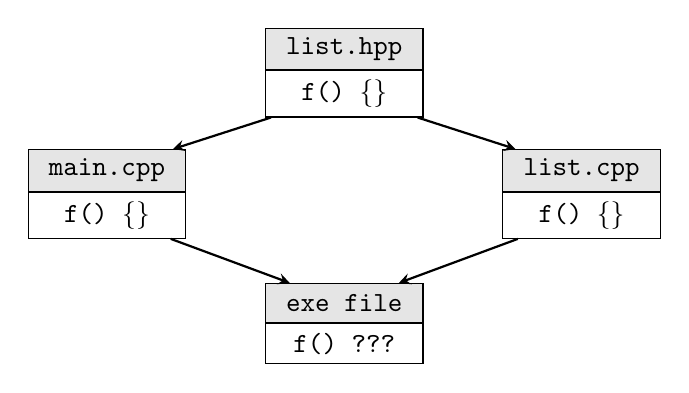
\begin{tikzpicture}
		\tikzstyle{HeaderName} = [rectangle, minimum width=2cm, minimum height=5mm, text centered, draw=black, fill= gray!20]
		\tikzstyle{CppName} = [rectangle, minimum width=2cm, minimum height=5mm, text centered, draw=black, fill= gray!20]
		\tikzstyle{FunctionName} = [rectangle, minimum width=2cm, minimum height=5mm, text centered, draw=black, fill= white]
		\tikzstyle{arrow} = [thick,->,>=stealth]
		
		
		\node (listHpp) [HeaderName] {\texttt{list.hpp}};
		\node (listHppF) [FunctionName, below = 0 mm of listHpp] {\texttt{f() \{\}}};
		
		\node (mainCpp) [CppName, below left = of listHpp] {\texttt{main.cpp}};
		\node (mainCppF) [FunctionName, below  = 0 mm of mainCpp] {\texttt{f() \{\}}};
		
		\node (listCpp) [CppName, below right = of listHpp] {\texttt{list.cpp}};
		\node (listCppF) [FunctionName, below  = 0 mm of listCpp] {\texttt{f() \{\}}};
		
		\node (exe) [CppName, below = 2.7 cm of listHpp] {\texttt{exe file}};
		\node (exeF) [FunctionName, below  = 0 mm of exe] {\texttt{f() ???}};
		
		\draw[arrow] (listHppF) -- (mainCpp);
		\draw[arrow] (listHppF) -- (listCpp);
		\draw[arrow] (mainCppF) -- (exe);
		\draw[arrow] (listCppF) -- (exe);
		\end{tikzpicture}
		\smallskip
		
		A \texttt{main.cpp}-ben vagy a \texttt{list.cpp}-ben lévő definíciója szerepeljen \texttt{f}-nek a futtatható fájlban?
	\end{figure}
	Az \texttt{f()} egy un. \textit{strong reference}-el jön létre ha nem inline, így a linker hibát dob ha több fordítási egységben definiálva van. Ha azonban inline-ként adjuk meg, akkor  \textit{weak reference}-ként értelmezi, a meglevő definíciók közül tetszőlegesen kerül egy kiválasztásra. Ez nyilván azt is jelenti, hogy minden ilyen függvény definíciójának meg kell egyeznie, hisz kellemetlen meglepetés érhet minket, ha különböző definíciók közül olyat választ a fordító, melyre nem számítanánk (és ez egyben nem definiált viselkedés is).
	\begin{note}
		A legtöbb fordítónál lehet egy LTO (\textit{link time optimalization}) funkciót bekapcsolni, mely a linkelésnél optimalizál, többek között ott végzi el az inlineolást.
	\end{note}
	\begin{note}
		Az inline függvények hajlamosak erősen megnövelni a bináris kódot, így az erőltetett használatuk nem javallott.
	\end{note}
	\begin{note}
		Az inline kulcsszó egy javaslat a fordítónak, de nem parancs. Nem inline függvények lehetnek inline-ok, és inlineként definiált függvények lehet mégsem lesznek azok.
	\end{note}
	Azok a tagfüggvények, melyek nem az osztály törzsében vannak definiálva, nem lesznek inline-ok, ezért volt az, hogy mielőtt szétszedtük a listánkat header fájlra és fordítási egységre, linkelési hibát kaptunk (\texttt{Iterator} és \texttt{ConstIterator} pár tagfüggvénye külön volt véve).
	\medskip
	
	Cseréljük le továbbá a print függvényt:
	
	\begin{lstlisting}
std::ostream& operator<<(std::ostream& os, const List &l)
{
	for(ConstIterator it = l.begin(); it != l.end(); ++it)
	{
		os << *it;
	}
	return os;
}
	\end{lstlisting}
	Sajnos fordítási hibát kapunk, hisz a fordító nem tudja mi az az \texttt{ostream}, így kell valamit include-olni. Ilyenkor a header fájlba inkább érdemes az \texttt{iosfwd} headert berakni \texttt{iostream} helyett, mert ez minden beolvasással és kiíratással kapcsolatos osztály/függvénynek csak a deklarációját tartalmazza, és így csökken a fordítási egység méretéte (azonban a cpp fájlban muszáj \texttt{iostream}-et használni, hogy a definíciók meglegyenek).
	\section{Névterek}
	
	A probléma csak az, hogy nagyon sok hasznos nevet elhasználtunk, pl. több \texttt{Iterator} nevű osztályt nem hozhatunk létre (az un. \textit{global namespace}-be kerültek), különben a névütközés áldozatai leszünk. Pedig várhatóan nem csak ennek az egy konténernek szeretnék iterátort írni. Megoldás lehet, hogyha az iterátorainkat egy névtérbe (\textit{namesspace}) rakjuk.
\begin{lstlisting}
namespace detail
{
	class Iterator
	{
		//...
	};
	class ConstIterator
	{
		//...
	};
}
\end{lstlisting}
	A névterek segíthetnek abba, hogy logikai egységebre rendezzük a programunkat. Az egyik legnagyobb ilyen egység az \texttt{std} névtér, mely tartalmaz minden függvényt, változót, stb, ami a standard részét alkotja. 
	
	Lehet névtereket egymásba is ágyazni, erre lehet példa a c++11-es \texttt{chrono} könyvtár, mely az \texttt{std} névteren belül számos dolgot a \texttt{chrono} alnévtérben tárol.
	
	\medskip
	Már csak az a baj, hogy így a \texttt{List} nem tudja, mi az az \texttt{Iterator}, hisz az egy \texttt{datail} nevű namespace-ben van, ezért vagy minden \texttt{Iterator}-t lecserélünk \texttt{detail::Iterator}-ra, vagy pedig létrehozunk egy szinonimát, melyet a \texttt{typedef} kulcsszóval tehetünk meg.
\begin{lstlisting}
class List
{
public:
	typedef detail::Iterator Iterator;
	typedef detail::ConstIterator ConstIterator;
	//...
};
\end{lstlisting}
	Ezzel a trükkel \texttt{List}-en belül (és csak ott!) elegendő lehet \texttt{Iterator}t írni. Ennek segítségével (mivel ezek a tpyedef-ek publikusak) így is lehet hivatkozni a \texttt{List} iterátorára: \texttt{List::Iterator}.
	
	\medskip
	Erre másik megoldás lehet, hogyha inline class-t hozunk létre, azaz az iterátor teljes deklarációját beillesztjük a \texttt{List}-be.
\begin{lstlisting}
class List
{
public:
	class Iterator
	{
		//...
	};
	//...
};
\end{lstlisting}
	\section{Nem template osztály átírása template osztályra}
	Már csak az a probléma, hogy ez az osztály csak \texttt{int}-ekre működik. Csináljunk belőle inkább egy template osztályt! Feladatunk csupán annyi, hogy az osztály elé írjunk egy \texttt{template <typename T>}-t, és minden \texttt{List}-et \texttt{List<T>}-re cseréljünk, és minden \texttt{int}-et \texttt{T}-re. Ehhez nyilván az iterátorainkat is módosítani kell.
	
	\medskip
	Időközben felmerül a hatékonyság kérdése is. A listánkban eddig mindent érték szerint vettünk át, ami \texttt{int}-nél (általában) hatékonyabb, mint a referencia szerinti, azonban template-eknél nem garantáljuk, hogy ilyen alap típussal fogják példányosítani az osztályunkat, és ilyenkor úgy szokás hozzáállni, hogy a leendő template paraméter egy nagyon nagy mérettel rendelkező típus lesz, melynél érték helyett konstans referenciával szokás átvenni minden paramétert hatékonyság végett. Sőt, még a \texttt{ConstIterator} dereferáló operátora is inkább konstans referenciát adjon vissza!
	\begin{note}
		Általában egy primitív típus, mint pl. az \texttt{int} vagy \texttt{char}, kisebb mérettel rendelkezik mint a hozzá tartozó pointer vagy referencia típus, így hatákonyabb ezeket a típusokat inkább érték szerint átvenni.
	\end{note}
	
	\fbox{\textbf{list.hpp:}}
\begin{lstlisting}
#ifndef LIST_H
#define LIST_H

#include <iosfwd>

template<typename T>
class List;

namespace detail 
{
	template<typename T>
	class Iterator
	{
	public:
		explicit Iterator(List<T> *p) : p(p) {}
		bool operator==(Iterator other) const { return p == other.p; }
		bool operator!=(Iterator other) const { return !(*this == other); }
		Iterator operator++();
		T &operator*() const;
	private:
		template<typename>
		friend class ConstIterator;
		List<T> *p;
	};
	
	template<typename T>
	class ConstIterator
	{
	public:
		ConstIterator(Iterator<T> it) : p(it.p) {}
		explicit ConstIterator(const List<T> *p) : p(p) {}
		bool operator==(ConstIterator other) const { return p == other.p; }
		bool operator!=(ConstIterator other) const { return !(*this == other); }
		ConstIterator operator++();
		const T &operator*() const;
	private:
		const List<T> *p;
	};	
}

template <typename T>
class List 
{
public:
	typedef detail::Iterator<T> Iterator;
	typedef detail::ConstIterator<T> ConstIterator;
	explicit List(const T &data_, List *next = 0) : data(data_), next(next) {}
	~List() { delete next; }
	List(const List &other);
	List &operator=(const List &other);
	void add(const T &data);
	Iterator begin() { return Iterator(this); }
	ConstIterator begin() const { return ConstIterator(this); }
	Iterator end() { return Iterator(0); }
	ConstIterator end() const { return ConstIterator(0); }
private:
	friend Iterator;
	friend ConstIterator;
	T data;
	List *next;
};

template<typename T>
std::ostream &operator<<(std::ostream& os, const List<T> &l);

#endif
\end{lstlisting}
	\fbox{\textbf{list.cpp:}}
\begin{lstlisting}
#include "list.hpp"
#include <iostream>

template<typename T>
List<T>::List(const List &other) : data(other.data), next(0) 
{
	if (other.next != 0) 
	{
		next = new List(*other.next);
	}
}

template<typename T>
List<T> &List<T>::operator=(const List<T> &other) 
{
	if (this == &other)
	return *this;
	delete next;
	data = other.data;
	if (other.next) 
	{
		next = new List(*other.next);
	} 
	else 
	{
		next = 0;
	}
	return *this;
}

template <typename T>
void List<T>::add(const T &data) 
{
	if (next == 0) 
	{
		next = new List(data);
	} 
	else 
	{
		next->add(data);
	}
}

namespace detail 
{
	template <typename T>
	Iterator<T> Iterator<T>::operator++() 
	{
		p = p->next;
		return *this;
	}
	
	template <typename T>
	T &Iterator<T>::operator*() const 
	{
		return p->data;
	}
	
	template <typename T>
	ConstIterator<T> ConstIterator<T>::operator++() 
	{
		p = p->next;
		return *this;
	}
	
	template <typename T>
	const T &ConstIterator<T>::operator*() const 
	{
		return p->data;
	}
}

template<typename T>
std::ostream &operator<<(std::ostream& os, const List<T> &l) 
{
	for(List<T>::ConstIterator it = l.begin(); it != l.end(); ++it) 
	{
		os << *it << ' ';
	}
	os << std::endl;
	return os;
}
\end{lstlisting}
	Itt a kiírató operátorunk miatt nem fog fordulni a kódunk! A \texttt{ConstIterator} {dependent scope}-ban lesz (ld. 7. gyakorlat).
	
	\begin{lstlisting}
template<typename T>
std::ostream &operator<<(std::ostream& os, const List<T> &l) 
{
	for(typename List<T>::ConstIterator it = l.begin(); it != l.end(); ++it) 
	{
		os << *it << ' ';
	}
	os << std::endl;
	return os;
}
	\end{lstlisting}
	
	\fbox{\textbf{main.cpp}}
	\begin{lstlisting}
#include <iostream>
#include "list.hpp"

int main() 
{
	List<int> head(5); // *
	head.add(8);
	head.add(10);
	head.add(8);
	std::cout << head;
}
	\end{lstlisting}
	
	Kérdés, hogy a megjelölt helyen kell-e typename vagy sem? A válasz az hogy nem, mert itt az \texttt{int} egy ismert típus, az előbbi példában meg \texttt{T} nem volt ismert, és az aztán bármi lehetett. A fordító a konkrét behelyettesítésnél tudni fogja, hogy \texttt{ConstIterator} egy típus lesz.
	
	\medskip
	No, fordítsunk!
	
	\medskip
	Igen, sejthető volt hogy ez nem fog menni. Úgy tűnhet, hogy semmi se úgy működik ebbe a nyelvbe, ahogy azt gondolnánk. Mindenre van magyarázat,
	\begin{center}
		\textit{,,néha az hogy valaki elkúrta.''}
		
		/Horváth Gábor/
	\end{center}
	Linkelési hibát kaptunk, de miért? A list.hpp-ben benne van mindenféle deklaráció, és a list.cpp-ben meg több \texttt{List}-béli implementáció. Amikor a list.cpp-t fordítjuk, létrejön az object fájl, a mainben szintén. Azonban minden implementált függvény template: a háttérben a list.cpp-ben semmit sem példányosítunk, így az szinte teljesen üres fordítás után. A main.cpp-ben így hiába megy az object fájl kreálása, lévén nem kell ismerni ahhoz a függvények definícióit, azonban a linkelésnél már meg kéne tudnunk találni azokat. Így a template osztályokat/függvényeket a header fájlokban kell tárolni.
	
	Itt megoldás lehet, hogyha az egész cpp-t beemeljük a list.hpp-be (itt mát azonban muszáj lesz az \texttt{iosfwd}-t \texttt{iostream}-re váltani). Az átláthatóság azonban nem lett áldozat, mert a fájl tetején van a deklaráció, és szétszedve van benne definíció.
	
	\section{STL konténerek}

	Az \textit{STL} a \textit{Standard Template Library} rövidítése.
	\subsection{Funktorok}
	Mielőtt belevetnénk magunkat az STL-ben lévő algoritmusokba és konténerekbe, fontos megismerkednünk a funktorokkal, melyek a rendezéseknél lesznek majd használatosak.
	\medskip
	
	A funktor egy olyan osztály, melynek túl van terhelve a gömbölyű zárójel operátora (tehát kvázi meg lehet hívni).
	
	\smallskip
	Egy egyszerű példa:
	\begin{lstlisting}
struct S
{
	int x;
	int operator()(int y)
	{
		return x + y;
	}
};
int main()
{
	S s1, s2;
	s1.x = 5;
	s2.x = 8;
	std::cout << s1(2) << std::endl; //7
	std::cout << s2(2) << std::endl; //10
}
	\end{lstlisting}
	Itt gyakorlatilag az objektum függvényként funkcionál. A funktorok azért fontosak, mert megadhatók template paraméterként, és így tudjuk elérni, hogy rendezéshez lehessen őket használni.
	\begin{note}
	Miért használunk funktorokat mondjuk függvénypointerek helyett? Világos, hogyha egyedi rendezést akarunk, akkor muszáj ezt az információt valahogy átadni. A funktorok erre alkalmasabbak, példaképp vegyük ehhez egy olyan template függvényt, melynek egyik template paramétere egy olyan funktort vár, melynek \texttt{()} operátora egy paramétert vár és \texttt{bool}-al tér vissza, és feladata az erre igazat adó elem megkeresése. 
	
	Hogyan tudnánk mi funktorok helyett függvénypointerrel a második páros számot megkeresni vele? Vagy az ötödik 8-al oszthatót? Nos, függvényekkel igencsak nehezen (kb statikus adattagokra kényszerülnénk, vagy egy hasonlóan nem épp elegáns megoldásra), azonban egy funktorban létrehozhatunk egy számlálót, melyet tudunk szépen növelgetni.
	\end{note}
	
	Segíthet a megértésben, ha tekintjük az alábbi példát:
	\begin{lstlisting}
template <class Compr>
bool f(int a, int b, Compr c)
{
	return c(a, b);
}

struct Less
{
	bool operator()(int a, int b) const
	{
		return a < b;
	}
};

int main()
{
	if( f(2,3, Less()) )
		std::cout << "2 kisebb mint 3! ";
	
	int a = 2, b = 2;
	if ( f(a, b, Less()) == false && f(b, a, Less()) == false )
		std::cout << "a es b egyenloek!" << std::endl;
}
	\end{lstlisting}
	Kimenet: \texttt{2 kisebb mint 3! a es b egyenloek!}
	
	Ez a funktor (\texttt{Less}) egy un. \textit{binary predicate}, azaz a gömbölyű zárójel operátora két azonos típusú objektumhoz rendel egy logikai értéket. Figyeljük meg, hogyan adtuk meg a harmadik paramétert: \texttt{Less}-nek meghívtuk a default konstruktorát, de nem adtunk neki változónevet. Itt egy un. névtelen temporális változó jön létre, mely \texttt{f} paramétereinek kiértékelésekor jön létre, majd az \texttt{f} lefutása után meg is semmisül. 
	
	Figyeljük meg azt is, hogy ebben az esetben érték szerint vettünk át: ez nem csak hatékonyabb, hisz \texttt{Less} mérete minimális (nincs adattagja), de mivel \texttt{Less()} egy jobbérték, csak így, vagy konstans referenciával tudnánk átvenni.
	\smallskip
	
	Ez alapján az egyenlőség is levezethető: \quad $a = b \quad \Leftrightarrow \quad \neg(a<b)\, \wedge\, \neg(b<a)$
	\medskip
	
	Könnyű látni, hogy általánosan beszélve, \texttt{Compr} összehasonlító funktorral $a$ és $b$ \texttt{T} típusú objektumoknál
	\[ a\ \ \text{és}\ \ b\ \ \text{ekvivalens}\quad \Leftrightarrow\quad \neg \,Compr(a, b)\, \wedge\, \neg \,Compr(b, a). \]
	\begin{note}
		Azokat a funktorokat, melyeknek az \texttt{()} operátora csak \textbf{egy} adott típusú objektumot várnak és \texttt{bool} a visszatérési értékük, \textit{unary predicate}-nek hívjuk.
	\end{note}

	\subsection{Bevezető a konténerekhez}
	C++ban az egyetlen tároló alapértelmezetten a tömb. Azonban az meglehetősen kényelmetlen: a tömb egymás mellett lévő memóriacímek összessége, nem tehetjük meg azt, hogy csak úgy hozzáveszünk 1-1 elemet (mi van ha valaki más már írt oda?). Ezért jobban járunk, ha írunk egy egyedi kontért (pl. az általunk létrehozott \texttt{List}), vagy pedig válogatunk az előre megírt STL konténerek között.
	
	Három konténertípust különböztetünk meg:
	\begin{itemize}
		\item Szekvenciális: Olyan sorrendben tárolja az adattagokat, ahogyan betesszük őket. \\Példa: \texttt{std::vector}, \texttt{std::deque,} \texttt{std::list.}
		\item Asszociatív: Az elemek rendezettek a konténerben.\\ Példa: \texttt{std::set}, \texttt{std::map}, \texttt{std::multiset}, \texttt{std::multimap}.
		\item Konténer adapter: Egy meglévő konténert alakítanak át, általában szogorítanak. Példaképp ha vesszük az \texttt{std::deque} konténert, ami egy kétvégű sor, könnyen tudunk belőle egy egyvégű sort csinálni. Ezen a konténerek általában egy másik konténert tárolnak, és annak a funkcióit szigorítják.
		\\Példa: \texttt{std::queue}, \texttt{std::stack}.
	\end{itemize}
	Minden STL konténer rendelkezik konstans és nem konstans iterátorral, fordított irányú és konstans fordított irányú iterátorral melyre így hivatkozhatunk:
	\begin{center}
		\setlength{\extrarowheight}{2pt}
		\begin{tabular}{|l|l|l|l|}
			\hline
			Iterátor típus&Ahogy hivatkozhatunk rájuk&Első elem&Past-the-end\\
			\hline
			\hline
			iterátor&\texttt{/*konténer név*/::iterator}&\texttt{begin()}&\texttt{end()}\\
			\hline
			konstans iterátor&\texttt{/*konténer név*/::const\_iterator}&\texttt{cbegin()}&\texttt{cend()}\\
			\hline
			fordított irányú&\multirow{2}{*}{\texttt{/*konténer név*/::reverse\_iterator}}&\multirow{2}{*}{\texttt{rbegin()}}&\multirow{2}{*}{\texttt{rend()}}\\
			iterátor&&&\\
			\hline
			fordított irányú&\multirow{2}{*}{\texttt{/*konténer név*/::reverse\_const\_iterator}}&\multirow{2}{*}{\texttt{crbegin()}}&\multirow{2}{*}{\texttt{crend()}}\\
			konstans iterátor&&&\\
			\hline
		\end{tabular}
	\end{center}
	
	A következő leírásban nem fogunk minden létező tagfüggvénnyel foglalkozni: egyrészt olyan sok van, hogy azt teljesen irreális észben tartani, másrészt sok ilyenhez érdemi hozzáfűznivalót én nehezen tudnék fűzni, így az egyes szekciók végén található link az adott konténerhez.
	
	\begin{note}
		Nagyon fontos képesség az is, hogy valaki hogyan tud utánanézni valaminek, amivel nincs teljesen tisztában, így erősen javallott a \url{cppreference.com}-el való ismerkedés, illetve más helyeken lévő információk böngészése is.
	\end{note}	
	\subsection{vector}
	A \texttt{<vector>} könyvtárban található, maga a konténer az \texttt{std::vector} névre hallgat. Bár a pontos definíciója értelemszerűen implementációfüggő, vannak olyan tulajdonságok, melyeket elvár a szabvány.
	\smallskip
	\begin{lstlisting}
#include <vector>
#inclide <iostream>

int main()
{
	std::vector<int> v;
	v.push_back(5); //v.size() == 1
	v.pop_back(); //v.size() == 0
	
	for (int i = 0; i<10; i++)
		v.push_back(i);
		
	for (std::vector<int>::iterator it = v.begin(); it != v.end(); ++it)
		std::cout << *it << std::endl; // 0 1 2 3 4 5 6 7 8 9
		
	for (int i = 0; i<v.size; i++)
		std::cout << v[i] << std::endl; // 0 1 2 3 4 5 6 7 8 9
}
	\end{lstlisting}
	A \texttt{vector} leggyakrabban dinamikusan lefoglalt tömbben tárolja az adatainkat, viszont a tömb mérete nem növelhető, így ha túl sok elemet akarunk beletenni, a \texttt{vector} lefoglal egy nagyobb memóriaterületet (leggyakrabban kétszer akkorát). Így a \texttt{push\_back}-nek a műveletigénye amortizált konstans: Általában konstans, de ha új memóriaterületet kell lefoglalni és a meglevő elemet átmásolni, akkor lineáris.
	
	\begin{note}
		Számos okból a \texttt{vector} a leggyakoribb választás, ha konténerre van szükségünk. Flexibilitása és gyorsasága kiemelkedő, azonban megvannak a maga gyenge pontjai.
	\end{note}
	
	\smallskip
	Előzménytárgyakból már ismerkedtünk ezzel a konténerrel: az előbb említett \texttt{push\_back} tagfüggvényt szoktuk használni új elem beszúrására a konténer végére, a \texttt{pop\_back} művelettel pedig a konténer végén lévő elemet tujuk kiszedni. 
	
	Feltűnhet, hogy ezek a műveletek, csakúgy mint számos egyéb melyet a cppreference-n olvashatunk, a konténer végére fókuszál, sőt, az elejére vonatkozó műveletek nincsenek is implementálva (nincs semmilyen \texttt{push\_front} vagy \texttt{pop\_front}). Ennek az az oka, hogy az \texttt{std::vector}-nál a konténer végének a módosítása a leghatékonyabb, ha a közepén/elején szeretnénk módosító művelteket végrehajtani, az gyakran a környező elemek odébb másolásával jár.

	\medskip
	Az \texttt{std::vector} tagfüggvényei, mint a nemsoká következő STL algoritmusok, többnyire iterátorokat várnak paraméterül. A következő példában töröljük ki a 4. elemet, majd szúrjuk is vissza!
	\begin{lstlisting}
int main()
{
	std::vector<int> v;
	for (int i = 0; i<10; i++)
		v.push_back(i);
		
	for (int i = 0; i<v.size(); i++)
		std::cout << v[i] << ' '; // 0 1 2 3 4 5 6 7 8 9
		
	std::vector<int>::iterator it = v.begin();
	++it; ++it; ++it;
	v.erase(it);
	for (int i = 0; i<v.size(); i++)
		std::cout << v[i] << ' '; // 0 1 2 4 5 6 7 8 9
	
	it = v.begin();
	++it; ++it; ++it; 
	v.insert(it, 3);
	for (int i = 0; i<v.size(); i++)
		std::cout << v[i] << ' '; // 0 1 2 3 4 5 6 7 8 9
}
	\end{lstlisting}
	\begin{note}
		Nyilván nonszensz, ahogy fent egyesével lépegettünk az iterátorral a negyedik elemig. Erre nemsokára egy értelmesebb megoldást fogunk látni.
	\end{note}
	Az iterátorok kezelésének azonban komoly veszélyei is vannak, a legnagyobb gonosz itt az un. iterátor invalidáció (\textit{iterator invalidation}). Amikor a \texttt{vector} által lefoglalt dinamikus tömb mérete túl kicsi az újabb elemek beszúrásához, és egy újabb tömbbe másolja át őket, minden iterátor, pointer és referencia ami a régebbi tömbre hivatkozott invalidálódik, lévén olyan területre hivatkoznak, melyeket már felszabadultak. 
	\smallskip
	
	Ugyanígy a konténer közepéről történő törlés, vagy a konténer közepére történő beszúrás is iterátor invalidációval jár.
	\smallskip
	
	Az invalidálódott objektumokkal végzett műveletek nem definiált viselkedést eredményeznek.
	\begin{lstlisting}
int main()
{
	std::vector<int> v;
	v.push_back(3);
	std::vector<int>::iterator it = v.begin();
	
	for (int i = 0; i<1000; i++)
		v.push_back(i);
		
	*it = 10; // nem definialt viselkedes
}
	\end{lstlisting}
	Az invalidáció elkerülése végett számos tagfüggvény egy iterátorral tér vissza, erre lehet példa az \texttt{insert}, mely az új elemre, vagy az \texttt{erase}, mely az utolsó eltávolított elem rákövetkezőjére hivatkozik.
	
	\smallskip
	Töröljünk egy vektorból minden páratlan számot!
	\begin{lstlisting}
int main()
{
	std::set<int> c = {1, 2, 3, 4, 5, 6, 7, 8, 9};
	for(std::vector<int>::iterator it = c.begin(); it != c.end(); )
	{
		if(*it % 2 == 1)
			it = c.erase(it);
		else
			++it;
	}
}
	\end{lstlisting}
	
	\medskip
	Link: \url{http://en.cppreference.com/w/cpp/container/vector}.
	
	\begin{note}
		Az \texttt{std::deque} működése ez alapján triviális, így annak megismerését az olvasóra bízom.
	\end{note}
	\subsection{set}
	
	Az \texttt{std::set} a \texttt{<set>} könyvtárban található. E konténernek nincs \texttt{push\_back} tagfüggvénye, helyette az \texttt{insert} függvény használatos elem betevésére. 
	\medskip
	
	Ez a konténer a matematikai halmazra hasonlít: egyedi elemet tárol, és ha egy eleve bent lévő elemmel ekvivalenset próbálnánk beszúrni, nem történne semmi. Ezen kívül a szabvány azt is megköveteli, hogy ez a konténer rendezett legyen, így a tárolandó \texttt{T} típus mellett egy olyan funktort is vár template paramterül, melynek \texttt{()} operátora két \texttt{T} típust vár paraméterül és logikai értékkel tér vissza.
	\smallskip
	
	Ez utóbbi template paramétert nem kell feltétlenül megadni, alapértelmezetten ugyanis az \texttt{std::set} az \texttt{std::less<T>} alapján rendez, mely gyakorlatilag az \texttt{<} operátorral ekvivalens.
	\smallskip
	
	Az \texttt{std::set} általában piros-fekete bináris faként van implementálva, a hatékonyság végett.
	\begin{note}
		A szabvány elvárja, hogy az \texttt{insert} műveletigénye logaritmikus legyen.
	\end{note}
	\begin{lstlisting}
#include <set>
#include <iostream>

struct Circle
{
	int x, y, r;
	Circle(int _x, int _y, int _r) : x(_x), y(_y), r(_r) {}
};

std::ostream& operator<<(std::ostream& os, const Circle &c)
{
	os << c.x << ' ' << c.y << ' ' << c.r;
	return os;
}

bool operator<(const Circle &lhs, const Circle &rhs)
{
	return lhs.r < rhs.r;
}

struct LessByX
{
	bool operator()(const Circle &lhs, const Circle &rhs) const
	{
		return lhs.x < rhs.x;
	}
};

int main()
{
	std::set<int> si;
	for(int i = 10; i>0; i--) //forditva!
		si.insert(i);
	//torlesrol majd kesobb
	//si.size() == 10
	si.insert(5); //si.size() == 10
	
	for(std::set<int>::iterator it = si.begin(); it != si.end(); ++it)
		std::cout << *it << ' '; // 0 1 2 3 4 5 6 7 8 9
	
	std::set<Circle> sk;
	sk.insert(Circle(3, 2, 2));
	sk.insert(Circle(1, 2, 1));
	sk.insert(Circle(2, 2, 3));
	for(std::set<Circle>::iterator it = sk.begin(); it != sk.end(); ++it)
		std::cout << *it << ", "; // 1 2 1, 3 2 2, 2 2 3
	
	std::set<Circle, LessByX> skr;
	skr.insert(Circle(3, 2, 2));
	skr.insert(Circle(1, 2, 1));
	skr.insert(Circle(2, 2, 3));
	for(std::set<Circle, LessByX>::iterator it = skr.begin(); 
												   it != skr.end(); ++it)
		std::cout << *it << ", "; // 1 2 1, 2 2 3, 3 2 2
}	
	\end{lstlisting}

	Egy egyedi rendezés használata veszélyekkel is járhat azonban.
	\begin{lstlisting}
struct strlen
{
	bool operator()(const std::string &lhs, const std::string &rhs) const
	{
		return lhs.length() < rhs.length();
	}
};

int main()
{
	std::set<std::string, strlen> s;
	s.insert("C++");
	s.insert("Java");
	s.insert("Haskell");
	std::cout << s.count("ADA") << std::endl; // 1
}
	\end{lstlisting}
	A \texttt{count} tagfüggvény megszámolja, hány \texttt{ADA}-val \textbf{ekvivalens} elem van a \texttt{set}ben. Mivel a funktorunk úgy hasonlít össze két elemet, hogy megnézi, melyik string hossza nagyobb, \texttt{C++} és az \texttt{ADA} ekvivalens lesz, így legnagyobb meglepődésünkre 1-et fog ez a program kiírni!
	%miért pocakos a dékán úr? mert has kell
\begin{lstlisting}
int main()
{
	std::set<std::string, strlen> s;
	s.insert("C++");
	s.insert("Java");
	s.insert("Haskell");
	s.insert("GOD");
	std::cout << s.size() << std::endl; // 3
}
\end{lstlisting}
	Most értelemszerűen azt várnánk, hogy a méret 4 legyen, de mégis 3at ír ki, mert az \texttt{insert} függvény nem teszi be a \texttt{GOD}-ot, lévén az a rendezés szerint a \texttt{C++}al ekvivalens.
\begin{lstlisting}
struct strlenWrong
{
	bool operator()(const std::string &lhs, const std::string &rhs) const
	{
		return lhs.length() <= rhs.length(); //ekvivalensek is lehetnek
	}
};

int main()
{
	std::set<std::string, strlenWrong> s;
	s.insert("C++");
	s.insert("Java");
	s.insert("Haskell");
	s.insert("ADA");
	std::cout << s.count("ADA") << std::endl; // 0
	std::cout << s.size() << std::endl; // 4
}
\end{lstlisting}
	Most figyeljük meg (emlékezzünk vissza dimatra), hogy egy szigorú rendezés helyett egy gyenge rendezést definiáltunk! Miért lehet ez problémás?
	
	\smallskip
	Helyettesítsünk be a rendezésünkbe.
	\[ \neg\big(\,a.length() \leq b.length()\,\big)\quad \wedge \quad \neg\big(\,b.length() \leq a.length()\,\big) \]
	Itt ha Ha a \texttt{C++}t és az \texttt{ADA}t behelyettesítsük, látjuk, hogy ez a formula hamisat ad, így nem bizonyulnak majd ekvivalensnek.
	
	Ha nem szigorú részben rendezést használunk, hanem gyengét, akkor a reflexivitást is elvesztjük. Ez azt jelenti, hogy egy elem nem lehet ekvivalens önmagával!
	
	Könnyen látható hogy a rendezésünk nem épp jó, mivel ha ekvivalenciát vizsgálunk, sose fog igazat adni, sose tudjuk meg, egy adott benne van-e, az elemek törlése se teljesen jó így.
	
	Link: \url{http://en.cppreference.com/w/cpp/container/set}
	
	\begin{note}
		Az \texttt{std::multiset} működése az eddigiek alapján triviális, így annak megismerését ismét az olvasóra bízom.
	\end{note}
	\subsection{list}
	Ez a konténer nagyon hasonló ahhoz, mint amit mi írtunk, csak lehet üres, és kétirányú.
	\smallskip
	
	Feltűnő lehet, hogy az \texttt{std::vector}-ral szemben ennek a konténernek nincs \texttt{[]} operátora, hiszen mire egy adott elemet elérünk, szépen el kell oda lépegetni egyesével. A szögletes zárójel operátort csak akkor szokás írni, hogy ha nagyon hatékony, lehetőleg konstans műveletigényű az adott elem lekérdezése, de ez a listánál nem teljesül.
	\begin{note}
		Bár elméletben gyorsabb egy láncolt listába beszúrni, de ez a gyakorlatban általában mégsem igaz. Azért, mert az egy dolog, hogy az elemeket egyesével odébb kell tolni egy vektorban, azonban mivel abban szekvenciálisan vannak a memóriacímek egymás mellett, és a processzor nem egyesével adja vissza az elemeit, hanem egy nagyobb blokkot mutat belőle, a vector sokkal gyorsabban végrehajtja ezeket a műveleteket, míg a listánál muszáj egyik címről a másikra haladni, ami sokkal költségesebb tud lenni.
	\end{note}
	\begin{note}
		Amennyiben sok elemből álló listánk van, és azok nagy objektumokat tárolnak, hatékonyabb lehet a \texttt{vector}-nál.
	\end{note}
	Hogyan tudunk akkor a harmadik elemre ugrani?
	\begin{lstlisting}
#include <iostream>
#include <list>

int main()
{
	std::list<int> l;
	for (int i = 0; i < 5; i++)
	l.push_back(i);
	std::list<int>::iterator it = l.begin();
	++it; ++it;
	std::cout << *it << std::endl; // 2
}
	\end{lstlisting}	
	Az iterátorok léptetésére kell hogy legyen egy egyszerűbb módszer. A fenti \texttt{std::vector}-ral tudnunk kéne ugorni azonnal a kívánt elemre, míg a listánál végig kell menni egyesével az elemeken: jó lenne egy olyan algoritmust találni, mely e kettőt egybefoglalja (erre később látunk is majd példát az STL algoritmusoknál).
	
	\medskip
	Ha böngészünk cppreference-en, feltűnhet, hogy az \texttt{std::vector}-ral szemben azonban létezik \texttt{push\_front} és \texttt{pop\_front} metódus: ezeket az \texttt{std::vector}-ral ellentétben konstans idő alatt el lehet végezni (elegendő a fejelemet a rákövetkező elemre állítani és kész is).
	\medskip
	
	Link: \url{http://en.cppreference.com/w/cpp/container/list}
	\subsection{map}
	Az \texttt{std::map} a \texttt{<map>} könyvtárban található. Ez egy egyedi kulcs-érték párokat tároló konténer, mely minden kulcshoz egy értéket rendel. Működése nagyon hasonlít az \texttt{std::set}-ére, annyi különbséggel, hogy párokat tárol (így két kötelező template paramétere van), és mindig a kulcs szerint rendez.
	\smallskip
	
	Van egy speciális beszúró függvénye is:
\begin{lstlisting}
#include <map>
#include <iostream>

int main()
{
	std::map<std::string, int> m;
	m["Hello"] = 42;
	m["xyz"] = 8;
	m["Hello"] = 9;
	std::cout << m.size() << std::endl; // 2
	std::cout << m["Hello"] << std::endl; // 9
}
\end{lstlisting}
	A \texttt{[]} operátor egy új kulcsot hoz létre, és ahhoz rendel egy új értéket. Az utolsó sornál mivel a \texttt{''Hello''}-t már tartalmazza a map, így annak az értékét felülírja.
	
	\medskip
	Sajnos ez az operátor azonban okozhat pár kellemetlen meglepetést is.
	\begin{lstlisting}
int main()
{
	std::map<std::string, int> m;
	std::cout << m.size() << std::endl; // 0
	if(m["c++"] != 0)
		std::cout << "nem 0" << std::endl;
	std::cout << m.size() << std::endl; // 1
}
	\end{lstlisting}
	A \texttt{[]} operátor úgy működik, hogy ha a \texttt{map} nem tartalmazza a paraméterként kapott kulcsot, akkor létrehozza és beszúrja, ha benne van, visszaadja az értékét. Bár mi nem tettük bele azt hogy \texttt{c++} szándékosan, de pusztán azzal, hogy rákérdeztünk, akaratlanul is megtettük. (Figyeljük meg, hogy akkor tudnánk új elemet hozzátenni, ha azt írnánk pl. hogy \texttt{m["C++"] = 3}; azonban mi nem adtunk meg ehhez a kulcshoz értéket. Ilyenkor a map alapértelmezett értéket rendel a kulcshoz, szám típusoknál 0-t, így be fog szúrni egy \texttt{("c++", 0)} párt.)
	\begin{lstlisting}
bool contains(const std::map<std::string, int> &m)
{
	//m["c++"]; forditasi hiba: [] operator nem konstans fuggveny.
	return m.find("C++") != m.end();
}
	\end{lstlisting}
	Ez a függvény helyesen vizsgálja, hogy a \texttt{c++} benne van-e. (Ha cppreference-en rákeresünk, a \texttt{map}-nek a \texttt{find} nevű tagfüggvénye egy iterátort ad vissza a talált elemre, illetve visszaadja egy past-the-end iterátort ha nem találja meg.)
	\medskip
	
	
	\texttt{std::map}-ban az iterálás kicsit trükkösebb, ugyanis \texttt{std::map} párokat tárol, méghozzá egy más alapból megírt struktúrát használ, az \texttt{std::pair}-t, ami kb. így néz ki:
	\begin{lstlisting}
template <typename T1, typename T2>
struct pair
{
	T1 first;
	T2 second;
};
	\end{lstlisting}
	Így az az adott kulcs ill. érték lekérdezése így fog kinézni:
	\begin{lstlisting}
for(std::map<std::string, int>::iterator i = m.begin(); i != m.end(); i++)
{
	std::cout << i->first << " " << i->second;
}
	\end{lstlisting}
	Amennyiben új elemeket szúrunk be, gyakran megkerülhető a problémás \texttt{[]} használata. Az \texttt{std::map} insert függvénye egy \texttt{std::pair}-t vár paraméterül, melyet könnyen tudunk alkotni \texttt{std::make\_pair} függvény segítségével.
	\begin{lstlisting}
std::set<int, char> s;
s.insert(std::make_pair(1, 'a'));
	\end{lstlisting}
	
	Link: \url{http://en.cppreference.com/w/cpp/container/map}
	\begin{note}
		Az \texttt{std::multimap} ehhez szintén hasonló, így gyakorlásként ezt ismét az olvasóra bíznám.
	\end{note}
	\section{Iterátor típusok}
	Korábban már elhangzott, hogy az általunk implementált \texttt{List}-hez tartozó \texttt{Iterator} és \texttt{ConstIterator} un. forward iterátorok. A forward iterator egy iterátor típus -- ebből több is van, és elengedhetetlenek az STL algoritmusok megértéséhez. 4 iterátor típust különböztetünk meg: input iterator, forward iterator, bidirectional iterator és random access iterator.
	\begin{itemize}
		\item Az \textbf{input iterator} típusokon legalább egyszer végig lehet menni egy irányba, továbbá rendelkeznek \texttt{++}, \texttt{*}, \texttt{==} és \texttt{!=} operátorral.
		\item A \textbf{forward iterator} típusokon többször is végig lehet menni, de csak egy irányba. Továbbá rendelkeznek \texttt{++}, \texttt{*}, \texttt{==} és \texttt{!=} operátorral.
		\item A \textbf{bidirectional iterator} típusokon többször is végig lehet menni, mindkét irányba. Továbbá rendelkeznek \texttt{++}, \texttt{$--$}, \texttt{*}, \texttt{==} és \texttt{!=} operátorral.
		\item A \textbf{random access iterator} típusokon többször is végig lehet menni, mindkét irányba, ezen felül a két iterátor között bármelyik elemre azonnal lehet hivatkozni. Továbbá rendelkeznek \texttt{++}, \texttt{
		$--$}, \texttt{*}, \texttt{==}, \texttt{!=}, \texttt{$-$} (két iterátor távolságát adja meg), összeadás \texttt{int}-el (paraméterként kapott mennyiségű elemmel előrelépés), kivonás \texttt{int}-el (hátralépés) operátorral/függvénnyel.
	\end{itemize}
	E listán látható, hogy pl. egy random access iterator sokkal flexibilisebb, és gyorsabb is, hisz bármikor bármelyik elemhez hozzáférhetünk, míg a mi listánk forward iteratora sokkal limitáltabb.
	
	\smallskip
	Az STL konténerek iterátorai is különböző iterator kategóriákban vannak:
	\begin{center}
		\setlength{\extrarowheight}{2pt}
		\begin{tabular}{|l|l|}
			\hline
			STL konténer&Iteratorának típusa\\
			\hline
			\hline
			\texttt{std::vector} & \multirow{2}{*}{\texttt{random access iterator}}\\
			\texttt{std::deque} &\\
			\hline
			\texttt{std::list} & \multirow{5}{*}{\texttt{bidirectional iterator}}\\
			\texttt{std::set} & \\
			\texttt{std::multiset} & \\
			\texttt{std::map} & \\
			\texttt{std::multimap} & \\
			\hline
		\end{tabular}
	\end{center}
	Világos, hogy egy flexibilisebb iterátorral több mindent meg tudunk tenni, vagy ugyanazt a funkciót hatékonyabban is meg tudjuk valósítani. Emiatt minden STL algoritmusnak (mint pl. az \texttt{std::find}) tudnia kell a template paraméterként kapott iterátor kategóriáját.
	\medskip
	
	Egy iterátornak úgy tudjuk a legegyszerűbben megadni a típusát, ha származunk az \texttt{std::iterator} típusból.
	\begin{note}
		Az öröklődés később lesz alaposabban boncolgatva, egyenlőre mondjuk azt, hogy az öröklődés követekztében mindent átpakolunk az \texttt{std::iterator} osztályból a mi iterátorunkba.
	\end{note}
	
	Link: \url{http://en.cppreference.com/w/cpp/iterator/iterator}
	\smallskip
	
	Látható hogy ennek osztálynak két kötelező template paramétere van, egy iterátor típus tag, és dereferáló operátor visszatérési értéke.
	
	\begin{lstlisting}
template <class T>
class Iterator : public std::iterator<std::forward_iterator_tag, T>
{
	//..
};

template <class T>
class ConstIterator : public std::iterator<std::forward_iterator_tag, T>
{
	//..
};
	\end{lstlisting}
	A cppreference-en megfigyelhető, hogy az \texttt{std::iterator} több typedef-et tartalmaz, mely jelöli hogy az iterátorunk milyen kategóriában van, milyen típussal tér vissza a dereferáló operátor, stb.
	\begin{note}
		Ennek alaposabb megértését az olvasóra bízom.
	\end{note}
	Így már fogjuk tudnuk majd használni az \texttt{STL} algoritmusokat is a konténereinken. 
	%TODO
%	\begin{note}
%		Ez egy baromi nagy dolog: létrehoztunk egy új adatszerkezetet, és ez tök jól együttműködik az eddigi algoritmusokkal.
%		
%		Azaz még viszonylag egyszerűen egy új függvényt is létre tudunk hozni, ami minden adatszerkezettel működni fog! C++ban az algoritmusok nem a konténereken működnek: lévén úgy szokás konténereket létrehozni, hogy írunk hozzá iterátort is, így elegendő egy algirtmusnak azt tudnia, hogy hogyan kell használni azt az iterátort. Emiatt várja el egy STL algoritmus, hogy közöüljük, milyen típusú iterátorunk van. Igaz, a konténereinkkel többet kell dolgoznunk, mert ezt az iterátort egyszer meg kell írni, de hosszú távon még így is rengeteg munkát tudunk megspórolni.
%	\end{note}
	
	\section{STL algoritmusok}
	\subsection{Bevezető az algortmusokhoz}
	Az STL algoritmusok az \texttt{<algorithm>} könyvtárban találhatóak, és számos jól ismert és fontos függvényt foglalnak magukba, mint pl. adott tulajdonságú elem keresése, partícionálás, szimmetrikus differencia meghatározása, stb.
	\medskip
	
	Az STL algoritmusok alap gondolatmenetét jól demonstrálja az alábbi példa : Írjunk egy függvény mely egy \texttt{std::vector<int>} konténernek a második adott értékű elemére hivatkozó iterátort ad vissza!
	\begin{lstlisting}
#include <vector>
#include <iostream>

typedef std::vector<int>::const_iterator VectIt;

VectIt findSecond(VectIt begin, VectIt end, const Val &v)
{
	while(begin != end && *begin != v)
	{
		++begin;
	}
	if (begin == end)
		return end;
	++begin;
	while(begin != end && *begin != v)
	{
		++begin;
	}
	return begin;
}

int main()
{
	std::vector<int> v;
	for (int i = 0; i<10; i++)
		v.push_back(i);
	v.push_back(5);
	std::vector<int>::iterator it = findSecond(v.begin(), v.end(), 5);
	if (it != v.end())
		std::cout << *it << std::endl; // 5
}
	\end{lstlisting}
	Amennyiben \texttt{findSecond} nem talál két \texttt{v}-vel ekvivalens elemet, egy past-the-end iterátort ad vissza.
	\begin{note}
		Lévén a konténert nem módosítjuk, bátran dolgozhatunk a nagyobb biztonságot nyújtó \texttt{const\_iterator}-ral.
	\end{note}
	Azonban könnyű látni, hogy egyáltalán nem fontos információ az algoritmus szempontjából, hogy a \texttt{vector} \texttt{int}-eket tárol.
	\begin{lstlisting}
template<class T>
typename std::vector<T>::const_iterator 
	findSecond(typename std::vector<T>::const_iterator begin, 
			   typename std::vector<T>::const_iterator end, 
			   const T &v)
{
	while(begin != end && *begin != v)
	{
		++begin;
	}
	if (begin == end)
		return end;
	++begin;
	while(begin != end && *begin != v)
	{
		++begin;
	}
	return begin;
}
	\end{lstlisting}
	Sajnos sikerült elég kilométer függvénydeklarációt sikerült írnunk, de a célt elértük.
	
	\smallskip
	Megállapítható, hogy itt még azt se kell tudnunk, minek az iterátorával dolgozunk, elegendő annyit tudnunk, hogy a \texttt{++} iterátorral lehet léptetni, és össze tudjuk hasonlítani őket az \texttt{!=} operátorral, azaz teljesítik egy input iterator feltételeit. Első körben vegyük az összehasonlítandó elem típusát külön template paraméterként.
	\begin{lstlisting}
template <class InputIt, class Val>
InputIt findSecond(InputIt begin, InputIt end, const Val &v)
{
	//...
}
	\end{lstlisting}
	Ezzel lényegében készen vagyunk, azonban egy apró módosítással elérhetjük hogy véletlenül se adjunk át olyan elemet harmadik paraméterként, mellyel a dereferált iterátor nem hasonlítható össze.
	\begin{note}
		Ez leginkább az \texttt{std::iterator}-ból való öröklés alkalmazását próbálja demonstrálni.
	\end{note}
	\begin{lstlisting}
template <class InputIt>
InputIt findSecond(InputIt begin, InputIt end, 
				   const typename InputIt::value_type &v)
{
	//...
}
	\end{lstlisting}
	
	Az STL algoritmusok iterátorokkal dolgoznak, azonban az, hogy minek az iterátorát használják, egyáltalán nem fontos tudniuk: elegendő annyi, hogy rendelkeznek azokkal az operátorokkal, melyeket fent felsoroltunk. Így például a mi listánk iterátorát ugyanúgy megadhatnánk a fenti függvények, mint egy \texttt{std::vector<int>}-ét.
	
	\medskip
	A korábban elhangzottak alapján implementáljunk egy függvényt, mely egy iterátort léptet előre: Amennyiben a paraméterként kapott iterátor kategóriája bidirectional iterator, egyesével lépegessünk a kívánt helyre, random access iterator esetén egyből ugorjunk oda.
	\begin{lstlisting}
template<typename BDIT> 
BDIT algorithm(BDIT it, int pos, std::bidirectional_iterator_tag) 
{
	for(int i = 0; i<pos; i++)
		++it;
	std::cout << "Slow" << ' ';
	return it;
}

template<typename RAIT>
RAIT algorithm(RAIT it, int pos, std::random_access_iterator_tag) 
{
	std::cout << "Fast" << ' ';
	return it + pos;
}

template<typename IT> 
IT advance(IT it, int pos) 
{
	typedef typename IT::iterator_category cat;
	return algorithm(it, pos, cat());
}

int main() 
{
	std::vector<int> v;
	std::list<int> l;
	for (int i = 0; i<10; i++)
	{
		v.push_back(i);
		l.push_front(i);
	}
	std::cout << *advance(v.begin(), 3) << std::endl; // Fast 3
	std::cout << *advance(l.begin(), 3) << std::endl; // Slow 6
}  
	\end{lstlisting}
	\medskip
	\begin{note}
		Az \texttt{std::vector} és \texttt{std::list}-nél felmerült iterátor lépegetésre találtunk megoldást: a fentihez hasonló működésű \texttt{std::advance} alkalmazható e célra.
	\end{note}
	Így tudjuk elérni azt, hogy különböző iterátor típusokra különböző algoritmust használjunk (bár nyilván ez jóval hatékonyabban van megoldva a standard könyvtárban).
	\medskip
	
	Ezek ismerétében vágjunk bele az STL algoritmusokba!
	\begin{note}
		Cppreference-en megfigyelhető, hogy irtózatosan sok algoritmus van -- csak úgy mint a konténereknél, a fontosabb algoritmusokról lesz szó, míg a többivel való ismerkedés gyakorlás végett az olvasóra bízom.
	\end{note}
	\subsection{find}
	Az \texttt{std::find} segítségével az első adott értékű elemre hivatkozó iterátort kaphatunk. Keressük meg a 4-el ekvivalens elemet!
	\begin{lstlisting}
int main()
{
	std::set<int> s;
	for(int i = 0; i<10; i++)
		s.insert(i);
	std::set<int>::iterator result = std::find(s.begin(), s.end(), 4);
	if (result != s.end())
		std::cout << *result << std::endl; // 4
	else
		std::cout << "4 nem eleme" << std::endl;
}
	\end{lstlisting}
	\begin{note}
		Lévén az \texttt{std::set} egy bináris fa, így várhatóan a keresést logaritmikus idő alatt is meg tudjuk tenni: ezért szokás az ilyen speciális konténereknek egyedi find függvényt írni, ami az \texttt{std::set} esetében egy tagfüggvény. 
	\end{note}
	\begin{lstlisting}
std::set<int>::iterator it = s.find(42);
if (i != s.end())
	//...
	\end{lstlisting}
	Azonban megállapítandó, hogy míg az \texttt{std::find} az \texttt{==} operátorral végzi az összehasonlítást, addig az \texttt{std::set} a template paraméterként kapott rendezéssel! (ami alapértelemzetten a \texttt{<} operátortól függ.)
\begin{lstlisting}
struct Circle
{
	int x, y, r;
	Circle(int _x, int _y, int _r) : x(_x), y(_y), r(_r) {}
};

bool operator<(const Circle &lhs, const Circle &rhs)
{
	return lhs.r < lhs.r;
}

bool operator==(const Circle &lhs, const Circle &rhs)
{
	return lhs.r == rhs.r && lhs.x == rhs.y && lhs.y == rhs.y;
}

int main()
{
	std::set<Circle> s;
	for(int i = 0; i<10; i++)
		s.insert(Circle(i, i + 1, i + 4));
	for(int i = 0; i<10; i++)
		s.insert(Circle(i, i + 1, i + 2));
	
	std::set<Circle>::iterator it1 = s.find(Circle(2, 3, 4));
	std::set<Circle>::iterator it2 = std::find(s.begin(), s.end(), 
														Circle(2, 3, 4));
	
	std::cout << it1->x << ' ' << it1->y << ' ' << it1->r; // 0 1 4
	std::cout << it2->x << ' ' << it2->y << ' ' << it2->r; // 1 9 10
}
\end{lstlisting}
	Ezzel semmi komolyabb gond nincs, de nem szabad meglepődni, amikor az ember ettől függően más megoldást kap mint amire számít.
	%TODO xazaxos rész
	\subsection{sort és stable\_sort}
	A következő példában próbáljuk rendezni egy \texttt{vector} elemeit!
	\begin{lstlisting}
std::vector<int> v {6,3,7,4,1,3};
std::set<int> s {6,3,7,4,1,3};
std::set<int> s1(v.begin(), v.end());
v.assign(s1.begin(), s1.end());
for(std::vector<int>::iterator it = v.begin(); it != v.end(); ++it)
{
	std::cout << *it << std::endl; // 1 3 4 6 7 
}
	\end{lstlisting}
%	for(int i : v)
%	{
%		std::cout << i << ' '; // 1 3 4 6 7 
%	}
%	
	\begin{note}
		Az fenti inicializálások a c++11-es újítás részei, sok magyarázatra gondolom nem szorulnak.
%		
%		A for ciklus szintén szokatlan lehet, ez is egy c++11es újítás, un. \textit{range-based for loop}. A fenti kód ezzel ekvivalens:
%		\begin{lstlisting}
%int i;
%for(std::vector<int>::iterator it = v.begin(); it != v.end(); it++)
%{
%	i = *it;
%	std::cout << i << ' ';
%}
%		\end{lstlisting}
%		Számunkra legyen elég most annyi, hogy az így írt ciklusok akkor működnek, ha a jobb oldalon álló objektum (most \texttt{v}) rendelkezik \texttt{begin()} és \texttt{end()} tagfüggvényekkel, vagy pedig az objektum egy tömb.
	\end{note}
	Most kihasználtuk, hogy az \texttt{std::set} alapértelmezetten rendezett: átpakoltuk az elemeket abba, majd visszaillesztettük az eredeti konténerbe. No persze, ez minden, csak nem hatékony. Ráadásul az egyik 3-as kiesett: az \texttt{std::set} megszűrte az elemet, mert ekvivalenseket nem tárol.
	
	\medskip
	Az ilyen jellegű barkácsolások sose fogadhatóak el hatékonyság szempontjából. Ismerkedjünk meg az ennél sokkal hatékonyabb \texttt{std::sort}-al!
	\begin{lstlisting}
std::vector<int> v {6,3,7,4,1,3};
std::sort(v.begin(), v.end());
for(std::vector<int>::iterator it = v.begin(); it != v.end(); ++it)
	std::cout << *it << ' '; // 1 3 3 4 6 7
	\end{lstlisting}
	Az \texttt{std::sort}, ha külön paramétert nem adunk neki, az \texttt{<} operátor szerint rendez.
	
	\medskip
	Rendezzük a fenti elemeket úgy, hogy a \texttt{>} operátor szerint legyenek sorban!
	\begin{lstlisting}
struct Greater
{
	bool operator()(int lhs, int rhs) const
	{
		return lhs > rhs;
	}
};

int main()
{
	std::vector<int> v {6,3,7,4,1,3};
	std::sort(v.begin(), v.end(), Greater());
	for(std::vector<int>::iterator it = v.begin(); it != v.end(); ++it)
		std::cout << *it << ' '; // 7 6 4 3 3 1 
}
	\end{lstlisting}
	\begin{note}
		Ez jól demonstrálja, hogy az \texttt{std::sort}, csak úgy mint a legtöbb STL algoritmus, számos overload-al rendelkezik.
	\end{note}
	Az \texttt{std::sort} az ekvivalens elemek sorrendjét nem (feltétlenül) tartja meg: rendezés után azoknak a sorrendje nem definiált.
	\begin{lstlisting}
struct StringLength
{
	bool operator()(const std::string &lhs, const std::string &rhs) const
	{
		return lhs.size() < rhs.size();
	}
};

int main()
{
	std::vector<std::string> v;
	v.push_back("ADA");
	v.push_back("Java");
	v.push_back("1234567");
	v.push_back("Maci");
	v.push_back("C++");
	v.push_back("Haskell");
	
	std::sort(v.begin(), v.end(), StringLength());
	
	for(std::vector<std::string>::iterator it = v.begin(); it != v.end(); ++it)
		std::cout << *it << ' ';
}
	\end{lstlisting}
	Lehetséges output: \texttt{C++, ADA, Java, Maci, Haskell, 1234567}.
	
	Amennyiben fontos, hogy az ekvivalens elemek relatív sorrendje megmaradjon, használjunk \texttt{std::sort} helyett \texttt{std::stable\_sort}-ot, mely pontosan ezt csinálja.
	\begin{note}
		Ennek nyilván ára is, van, általában az \texttt{std::stable\_sort} kevésbé hatékony.
	\end{note}
	
	Link: \url{http://en.cppreference.com/w/cpp/algorithm/sort}.
	\subsection{remove}
	Az \texttt{std::remove} algoritmus a konténerben lévő elemek törlését segíti elő. Töröljük ki egy vectorból az összes 3-al ekvivalens elemet!
	\begin{lstlisting}
std::vector<int> v{1,2,3,3,4,5,6};
std::cout << v.size() << std::endl; // 7
std::remove(v.begin(), v.end(), 3);
std::cout << v.size() << std::endl; // 7
	\end{lstlisting}
	Legnagyobb meglepetésünkre, ez semmit se fog törölni: az \texttt{std::remove} átrendezi a konténert, úgy hogy a konténer elején legyenek a nem törlendő elemeket, és utána a törlendőek, és az első törlendő elemre visszaad egy iterátort. Ennek segítségével tudjuk, hogy ettől az iterátortól a past-the-end iteratorig minden törlendő.
	\begin{lstlisting}
std::vector<int> v{1,2,3,3,4,5,6};
std::cout << v.size() << std::endl; // 7
auto it = std::remove(v.begin(), v.end(), 3);
v.erase(it, v.end());
std::cout << v.size() << std::endl; // 5
	\end{lstlisting}
	\begin{note}
		Ebben a kódban van pár c++11-es újítás is: az \texttt{auto} kulcsszó megadható konkrét típus helyett. Ilyenkor az egyenlőségjel bal oldalán lévő objektum típusára helyettesítődik a kulcsszó. Példaképp, fent a fordító meg tudja határozni, hogy az \texttt{std::remove}-nak a visszatérési értéke itt \texttt{std::vector<int>::iterator} lesz, így a kód azzal ekvivalens, mintha ezt írtuk volna:
		
		{\centering\texttt{std::vector<int>::iterator it = std::remove(v.begin(), v.end(), 3);} \par}
		
		Bár az \texttt{auto} kulcsszót sokáig lehetne még boncolgatni, legyen annyi elég egyenlőre, hogy a template paraméter dedukciós szabályok szerint működik (c++11et nem szükséges tudni a vizsgához).
	\end{note}
	\subsection{Végszó az algoritmusokhoz}
	Megjegyzendő, hogy nem minden algoritmus működik minden iterátor típussal (pl. az \texttt{std::sort} random access iteratort vár), és vannak egyes algoritmusok, melyeknek speciális előfeltételei is vanak (például az \texttt{std::unique} egy rendezett konténert vár).
	\medskip
	
	Fontos az is, hogy ezek az algoritmusok általában nagyon hatékonyak, így gyakran nem is érdemes saját magunktól megírni.
	
	\medskip
	Gyakran nincs szükség arra, hogy a függvénynevek elé kiírjuk, melyik névtérből származnak.
	\begin{lstlisting}
//...
auto it = remove(v.begin(), v.end(), 3);
//...
	\end{lstlisting}
	Itt a fordító a függvény paraméterekből ki tudja találni , hogy milyen névtérből van az algoritmus. Ezt \textit{Argument Dependent Lookup}-nak nevezzük, vagy röviden ADL-nek. Mivel a \texttt{vector} ugyanúgy az \texttt{std} névtérből származik, és azt adtunk meg paraméternek, tudni fogja a fordító, hogy a \texttt{remove}-ot is abban a névtérben kell keresni.
	
	\subsection{Gyakorló feladat}
	
	Vegyünk egy konténert, és jelöljünk meg benne bár elemet, melyektől azt szeretnénk, hogy legyenek egymás mellett, de minden más elem sorrendje ne változzon.
	\begin{center}
		\begin{tabular}{|c|c|c|c|c|c|c|c|}
			\hline
			&&*&&*&*&&*\\
			\hline
		\end{tabular}
		
		$\Downarrow$
		
		\begin{tabular}{|c|c|c|c|c|c|c|c|}
			\hline
			&&*&*&*&*&&\\
			\hline
		\end{tabular}
	\end{center}
	Próbáljuk a csillaggal jelölt elemet egymás mellé tenni: ezt megtehetjük pl. két \texttt{stable\_partition}-nel, mert az ekvivalens elemek sorrendjét nem változtatják. 
	
	Most csináljuk azt, hogy a kijelölt elemek a konténer végén legyenek, de a többi elem sorrendje ne változzon! Itt használhatjuk az előbbi algoritmusok után az \texttt{std::rotate}-et.
	\begin{center}
		
		\begin{tabular}{|c|c|c|c|c|c|c|c|}
			\hline
			&&*&*&*&*&&\\
			\hline
		\end{tabular}
		
		$\Downarrow$
		
		\begin{tabular}{|c|c|c|c|c|c|c|c|}
			\hline
			&&&&*&*&*&*\\
			\hline
		\end{tabular}
	\end{center}
	\begin{center}
		\textit{,,Általában az emberek nem szeretik, hogyha kicsesznek velük, és ha kicseszel a kollégáiddal, morcosak lesznek''}
		
		/Horváth Gábor/
	\end{center}
	\section{Objektum orientált programozás}
	Objektum orientált programozásnál e hármat várjuk el:
	\begin{itemize}
		\item enkapszuláció
		\item kód újrafelhasználás
		\item adat elrejtés
	\end{itemize}
	Az, hogy egy adott nyelv ezt hogyan valósítja meg, az a saját maga dolga. Vannak nyelvek, melyek jobban alkalmasan objektum orientált programozásra, mint mások. Példaképp, a C nyelvre is mondhatjuk, hogy objektum orientált, bár nincs benne örökölődés, és nem igazán kézenfekvő az adatok elrejtése sem (bár lehetséges). Nyilvánvalóan ennél egyel praktikusabb nyelvek is léteznek, példaképp Java, és nyilván a c++ is, melyek sokkal erősebb nyelvi eszközökkel rendelkeznek ezek megvalósítására.
	
	Fontos, hogy az objektum orientáltság fogalmát ne csak az osztályokhoz kössük!
	
	\subsection{Öröklődés (\textit{inheritance})}
	Tekintsük az alábbi kódot:
	\begin{lstlisting}
class Sikidom
{
	int x;
	int y;
public:
	Sikidom(int x, int y) : x(x), y(y) {}
	double terulet() const
	{
		//...
	}
};
	\end{lstlisting}
	Itt a célunk egy általános síkidom megadása, azonban bajban vagyunk, hisz nem tudjuk megmondani, hogy épp egy tetszőleges síkidomnak milyen lesz a területe. Hozzunk létre egy kört, hisz annak a területét meg tudjuk adni! Próbáljuk ehhez használni az öröklődést: vegyünk át mindent, ami a Síkidomban van, elvégre minden kör egy síkidom!
	
	\begin{lstlisting}
class Kor : public Sikidom
{
	double r;
public:
	double terulet() const
	{
		return r * r * 3.14;
	}
};
	\end{lstlisting}
	Az öröklődés következtében \texttt{Kor} osztály \texttt{Sikidom} összes adattagját és metódusát átveszi. Fentebb látható az öröklődés szintaktikája: kettőspont, és utána egy öröklődési típus (ez esetben \texttt{public}, erről nemsoká lesz bővebben szó). Mondhatjuk azt is, hogy a \texttt{Kor} \textit{az egy} \texttt{Sikidom}, hisz minden, a \texttt{Sikidom}ra jellemző tulajdonsággal rendelkezik.
	\begin{note}
		Nagyon fontos, hogy a 3,14-nél pontot és nem vesszőt használunk. Ha ezt írnánk:
		\begin{lstlisting}
int i = 1, 2, f(), g();
		\end{lstlisting}
		
		Akkor rendre a vessző paraméter előtti tag mindig kiértékelődik, és utána értékeli ki a következőt, a korábbi eredményt meg elhajítja. A végén az egész azzal lesz ekvivalens, mintha simán azt írnánk, hogy \texttt{int i = g();}.
		
		Egy fél mondat erejéig jegyezzük meg azt is, hogy lebegőpontos számokat sose hasonlítsunk össze! Jusson eszünkbe, ami Numerikus Módszereken hangzik el: minden lebegőpontos szám tartalmazhat egy kis pontatlanságot.
		\begin{lstlisting}
for (double d = 0; d != 1; d += 0.1)
{
	std::cout << d << ' ';
}
		\end{lstlisting}
		Itt bár azt várnánk, hogy a kimenet \texttt{0 0.1 0.2 ... 1.0} legyen, legnagyobb valószínűséggel végtelen ciklusba futunk. Ez amiatt van, hogy a 0.1 (várhatóan) tartalmaz egy kis pontatlanságot, és így hiába írja ki  a programunk hogy \texttt{d} értéke 1, az várhatóan csak nagyon közel lesz hozzá.
	\end{note}
	Az, hogy publikusan örököltünk (erre volt a \texttt{public} kulcsszó), azt jelenti, hogy egy {altípus}-t (\textit{subtype}) hoztunk létre. 
	Ezt azt is jelenti, hogy minden helyre, ahol \texttt{Sikidom}-ot szeretnénk használni, \texttt{Kor}-t is használhatunk.
	
	Van egy apróbb probléma a fenti kóddal azonban: Az osztály azon adattagjai, melyek \texttt{private}-ként vannak deklarálva, csak az adott számára elérhetőek.
	
	Ez probléma hisz mi \texttt{Kor}-t azért hoztuk létre, hogy speciálisabb feladatokat tudjuk végrehajtani \texttt{Sikidom} tulajdonságaival, azonban \texttt{x} és \texttt{y} privát, és csak \texttt{Sikidom} tud hozzáférni. Írjuk át ezt protectedre:
\begin{lstlisting}
class Sikidom
{
protected:
	int x;
	int y;
public:
	Sikidom(int x, int y) : x(x), y(y) {}
	double terulet() const {}
};
\end{lstlisting}
	A \texttt{protected} tagokhoz csak az adott osztály fér hozzá, és azon osztályok, melyek ebből örökölnek. Nem csak publikusan tudunk örökölni, \texttt{protected}-del, és \texttt{private}-el is. Az alábbi táblázat mutatja, hogy az származott osztály (\textit{derived class}) milyen adattagokhoz fér hozzá a bázisosztályból (\textit{base class}) különböző öröklődési típusok esetén:
	\begin{center}
		\setlength{\extrarowheight}{2pt}
		\begin{tabular}{|c||c|c|c|}
			\hline
			Öröklődés típusa:&public&protected&private\\
			\hline
			\hline
			Saját adatok/metódusok& \cellcolor{green!20}igen&\cellcolor{green!20}igen&\cellcolor{green!20}igen\\
			\hline
			Örökölt adatok/metódusok (public)&\cellcolor{green!20}igen&\cellcolor{green!20}igen&\cellcolor{green!20}igen\\
			\hline
			Örökölt adatok/metódusok (protected)&\cellcolor{green!20}igen&\cellcolor{green!20}igen&\cellcolor{green!20}igen\\
			\hline
			Örökölt adatok/metódusok (private)&\cellcolor{red!20}nem&\cellcolor{red!20}nem&\cellcolor{red!20}nem\\
			\hline
		\end{tabular}
	\end{center}
	Ez pedig mutatja egy adott adattag/metódus védettségét öröklődés után:
	\begin{center}
		\begin{tabular}{|c||c|c|c|}
			\hline
			Öröklődés típusa:&public&protected&private\\
			\hline
			\hline
			Örökölt adatok/metódusok (public)&\cellcolor{green!20}public&\cellcolor{orange!20}protected&\cellcolor{red!20}private\\
			\hline
			Örökölt adatok/metódusok (protected)&\cellcolor{orange!20}protected&\cellcolor{orange!20}protected&\cellcolor{red!20}private\\
			\hline
			Örökölt adatok/metódusok (private)&\cellcolor{red!20}private&\cellcolor{red!20}private&\cellcolor{red!20}private\\
			\hline
		\end{tabular}
	\end{center}
	Az öröklődés típusa ha \texttt{class}ból öröklünk \texttt{private}, ha \texttt{struct}ból akkor \texttt{public.}
	\begin{note}
		A publikus öröklődést szokás {az egy} (\textit{is a}), privátot \texttt{van egy} (\textit{has a}) kapcsolatnak is hívni.
	\end{note}
	Picit térjünk visza a fenti értékadáshoz, mert ott azért van még mit megbeszélni.
	\begin{lstlisting}
Kor k;
Sikidom s;
s = k; //ok
	\end{lstlisting}
	Azt már letisztáztuk, hogy \texttt{Kor} \texttt{Sikidom} altípusa, de azonban ez akkor is két különbötő típus, hogyan lehet, hogy nem kapunk fordítási idejű hibát?
	
	A válasz az, hogy a fordító meg tudja oldani e két típus közötti értékadást. Mivel \texttt{Kor}-ben benne van maga \texttt{Sikidom} is, ezért meghívja az ahhoz tartozó értékadó operátort, és a \texttt{Kor}-ben lévő \texttt{Sikidom}-ot adja majd értékül.
	
	Ez azonban magával hordozza azt is, hogy minden információ, ami \texttt{Kor}-respecifikus (pl. sugár (\texttt{r})) elveszik. Ez az un. \textit{slicing}. Ebben az esetben, lévén a fordító generálta nekünk az értékadó operátort, és az alapértelmezetten minden adattagra meghívja az arra definiált értékadó operátort, gyakorlatilag ez fog történni:
	\begin{lstlisting}
s.x = k.x;
s.y = k.y;
	\end{lstlisting}
	
	Ezt a \textit{slicing} dolgot meg tudjuk kerülni, ha egy pointert hozunk létre: Hisz egy \texttt{Sikidom}-ra mutató pointer mutathat \texttt{Kor}-re is, és mivel az ''csak'' mutogat, nem fog levágni semmit (referenciák szintén!). 
	\begin{lstlisting}
Kor k;
Sikidom *sp = &k; 
Sikidom &sr = k;
	\end{lstlisting}
	Így minden adathoz, ami \texttt{Kor}-ben \texttt{Sikidom}-tól lett örökölve, hozzá tudunk férni \texttt{sp}-n keresztül. Fontos megjegyeznünk azonban, hogy egy \texttt{Sikidom} típusú pointer csak ''\texttt{Sikidom}nyi'' adattagokat/metódusokat tud kezelni.
	
	Mi fog történni, ha meghívjuk a \texttt{terulet} metódust?
	\begin{lstlisting}
Kor k;
Sikidom *sp = &k;
sp->terulet();
	\end{lstlisting}
	Itt azt fogjuk tapasztalni, hogy \texttt{Sikidom} függvénye fog meghívódni. Ennek oka az, hogy \texttt{sp} statikus típusa (\textit{static type}) az \texttt{Sikidom}, és hatékonyság végett alapértelmezetten mindig a statikus típushoz tartozó függvényt hívódik meg. Egy pointernek azonban van un. dinamikus típusa is (\textit{dynamic type}), ami ebben az esetben \texttt{Kor} lesz. A dinamikus típust csak futási időben lehet ismert, hisz lehetetlen azt megállapítani fordítási időben, hogy milyen típusú objektumra fog mutatni az \texttt{sp}. Ha mindig a dinamikus típus szerint hívná meg a program függvényeket, annak nagy futási idejű költsége lenne. Ahhoz, hogy rákényszerítsük a fordítót arra, hogy a dinamikus típus szerint fordítson, használnunk kell a \texttt{virtual} kulcsszót.
	%TODO miért szar a láncolt lista: túl költséges a processzorba pakolás ...
	\subsection{Virtuális függvények}
	Azokat az osztályokat, melyek legalább egy virtuális függvénnyel rendelkeznek, polimorfikus osztálynak (\textit{polymorphic class}) nevezzük.
\begin{lstlisting}
class Sikidom
{
protected:
	int x;
	int y;
public:
	Sikidom(int x, int y) : x(x), y(y) {}
	virtual double terulet() const //virtualis!
	{
		//...
	}
};

class Kor : public Sikidom
{
	double r;
public:
	double terulet() const
	{
		return r * r * 3.14;
	}
};
\end{lstlisting}
	Picit bánthat minket az, hogy hogyan jöhet elő ez a probléma, ugyanis úgy tűnik, mintha sértenénk a \textit{one definition rule}-t, hisz létrehoztunk két függvényt azonos visszatérési értékkel és paraméterlistával: a kiút az, hogy itt felüldefiniálás (\textit{override}) fog bekövetkezni, azaz a \texttt{Kor}-béli \texttt{terulet} le fogja árnyékolni a \texttt{Sikidom} \texttt{terulet} függvényét. Viszont ez a leárnyékolás nem ér sokat, ha nincs \texttt{virtual} kulcsszó, és ha egy \texttt{Sikidom} típusú pointerrel akarjuk ezt használni.
	
	A bázisosztály függvényének leárnyékolása azonban nem azt jelenti, hogy azt a függvényt nem lehet meghívni. Ha explicit módon jelezzük a fordítónak, hogy a bázisosztályban definiált metódust szeretnénk meghívni, akkor minden virtualitás ellenére is az lesz meghívva:
	\begin{lstlisting}
int main()
{
	Kor k;
	std::cout << k.Sikidom::terulet();
}
	\end{lstlisting}
	Ezt explicit névfeloldásnak (\textit{explicit scope resolution}) nevezzük.
	\begin{note}
		Minden metódus, mely öröklődésnél a bázisosztály egy virtuális metódusával megegyező visszatérési értékkel, paraméterlistával és konstanssággla rendelkezik, implicit módon virtuális lesz. (pl.: \texttt{Kor}-ben \texttt{terulet} implicit módon virtuális lesz, mert \texttt{Sikidom}-ban is az volt)
	\end{note}
	Konstruktor sose lehet virtuális.
	\subsection{Tisztán virtuális függvények}
	Bár ha háromszögekre felvágunk egy síkidomot, meg tudjuk mondani a területét, azért látjuk, hogy iszonyatos szenvedés nélkül egy általános síkidom területének megadása aligha lehetséges. Ezért gyakran úgy dönthetünk, hogy egy adott függvénynek csak a felületét (\textit{interface}) örököltetjük, de implementációját nem.
	
	A fenti osztálynál azonban probléma, hogyha valaki létrehoz egy \texttt{Sikidom} típusú objektumot, és meghívja a \texttt{terulet} függvényt, jogosan várja, hogy az ki is számítsa neki. Ennek megkerülésére alkalmazahtunk egy trükköt: \texttt{Sikidom}ban \texttt{terulet}-et tisztán virtuálissá tesszük:
	
\begin{lstlisting}
class Sikidom
{
protected:
	int x;
	int y;
public:
	Sikidom(int x, int y) : x(x), y(y) {}
	virtual double terulet() const = 0;
};
\end{lstlisting}
	Mostmár \texttt{terulet} tisztán virtuális (\textit{pure virtual}) \texttt{Sikidom}-ban. Az olyan osztályokat, melyekből nem lehet objektumot létrehozni, absztraktnak nevezzük. Az olyan osztályokból, melyek tartalmaznak tisztán virtuális metódusokat, nem tudunk objektumot létrehozni.
	\begin{note}
		Egy osztály úgy is lehet absztrakt, hogy \texttt{protected}-dé tesszük a konstruktorait (erről majd később). Az egyszerűség kedvéért, ha absztrakt osztályról beszélünk, gondoljunk egy tisztán virtuális metódussal rendelkező osztályra.
	\end{note}
	Egy olyan osztály, mely egy absztrakt osztályból örököl, ahhoz, hogy példányosítható legyen (lehessen olyan típusú objektumokat létrehozni), felül kell írnia az összes abban található tisztán virtuális függvényt.
	\begin{lstlisting}
int main()
{
	Sikidom s; //nem ok, forditasi ideju hiba
	Kor k; //ok
	Sikidom *sp = &k;
	Sikidom &sr = k;
	
	sp->terulet();
	sr.terulet();
}
	\end{lstlisting}
	Mint láthatjuk, absztrakt típusú pointert és referenciát lehet létrehozni, így a polimorfizmus összes előnyével élhetünk, továbbá mindenkit sikerült rákényszeríteni a \texttt{terulet} függvény definiálására, aki \texttt{Sikidom}-ból örököl.
	
	Persze, ettől mi még írhatunk definíciót egy tisztán virtuális függvényhez:
\begin{lstlisting}
class Sikidom
{
protected:
	int x;
	int y;
public:
	Sikidom(int x, int y) : x(x), y(y) {}
	virtual double terulet() const = 0;
};

double Sikidom::terulet()
{
	return 0;
}
\end{lstlisting}
	Figyeljük meg, hogy egy tisztán virtuális függvényt csak a deklarációtól külön tudunk definiálni. 
	
	Ez a trükk például akkor hasznosítható, ha egy van egy absztrakt bázisosztályunk, melynek szeretnénk, hogy öröklés után egy függvényét mindenki definiáljon felül, de akarunk adni hozzá egy alap implementációt.
\begin{lstlisting}
class Kor : public Sikidom
{
	double r;
	public:
	double terulet() const
	{
		return Sikidom::terulet();
	}
};
\end{lstlisting}
	
	A későbbiekben tekintsünk \texttt{Sikidom}-ra úgy, mintha nem lenne tisztán virtuális függvénye.
	\subsection{Kód módosítása polimorfizmusnál}
	\smallskip
	Szánjunk pár szót meglévő kód módosításáról, ha polimorfizmusról is van szó.
	\begin{lstlisting}
void f(Kor* k)
{
	//...
}
	\end{lstlisting}
	Lehet, az implementáció egy pontján úgy döntünk, hogy ez várjon inkább síkidomokat.
	\begin{lstlisting}
void f(Sikidom* k)
{
	//...
}
	\end{lstlisting}
	Ezzel semmi gond nem lesz, ugyanis ha mi \texttt{f}-nek továbbra is \texttt{Kor}öket fogunk adni, egy \texttt{Sikidom} típusú pointer tud még mutatni \texttt{Kor} típusra. Ennek a tanulsága az, hogy paramétereknél \textbf{felfelé} az öröklődési láncon lehet haladni, lefelé nem, hiszen egy síkidomra mutató pointer mutathat körre, de fordítva nem. Továbbá, ha visszatérési értéknél:
	\begin{lstlisting}
Sikidom f(...) {}
	\end{lstlisting}
	úgy döntünk, inkább kört adunk vissza:
	\begin{lstlisting}
Kor f(...) {}
	\end{lstlisting}
	nem lesz semmi gond, hisz itt is, minden kör \textit{az egy} síkidom. Azaz ha módosítjuk egy függvény visszatérési értékét, \textbf{lefelé} haladjunk az öröklődési ágon.
	\begin{lstlisting}
Kor *k;
Sikidom * sp = f(k);
	\end{lstlisting}
	Bajban lennénk, ha \texttt{Sikidom}-nál egy általánosabb osztályt adna vissza \texttt{f}.
	\medskip
	
	Legyen adott egy osztályhierarchia, melyben \texttt{B} publikusan örököl \texttt{A}-ból, \texttt{C} osztály \texttt{B}-ből, és végül \texttt{D} osztály \texttt{C}-ből. Ilyenkor \texttt{A} a ,,legáltalánosabb'' osztály, és \texttt{D} a ,,legspeciálisabb''.
	
	Az alábbi táblázat jól összefoglalja az itt megállapítottakat (piros: a módosítás nem megfelelő, zöld: a módosítás jó lesz):
	\begin{center}
		\setlength{\extrarowheight}{2pt}
		\begin{tabular}{|l||c|c|c|c|}
			\hline
			&Eredeti típus&\multicolumn{3}{c|}{Módosított típus}\\
			\hline
			\hline
			\multirow{4}{*}{Paraméterek}&A*&\cellcolor{red!20}B*&\cellcolor{red!20}C*&\cellcolor{red!20}D*\\
			\cline{2-5}
			&B*&\cellcolor{green!20}A*&\cellcolor{red!20}C*&\cellcolor{red!20}D*\\
			\cline{2-5}
			&C*&\cellcolor{green!20}A*&\cellcolor{green!20}B*&\cellcolor{red!20}D*\\
			\cline{2-5}
			&D*&\cellcolor{green!20}A*&\cellcolor{green!20}B*&\cellcolor{green!20}C*\\
			\hline
			\hline
			\multirow{4}{*}{Visszatérési érték}&A*&\cellcolor{green!20}B*&\cellcolor{green!20}C*&\cellcolor{green!20}D*\\
			\cline{2-5}
			&B*&\cellcolor{red!20}A*&\cellcolor{green!20}C*&\cellcolor{green!20}D*\\
			\cline{2-5}
			&C*&\cellcolor{red!20}A*&\cellcolor{red!20}B*&\cellcolor{green!20}D*\\
			\cline{2-5}
			&D*&\cellcolor{red!20}A*&\cellcolor{red!20}B*&\cellcolor{red!20}C*\\
			\hline
		\end{tabular}
	\end{center}
	\subsection{Többszörös öröklődés}
	C++ban lehetőségünk van többszörösen örökölni. Ez azt jelenti, hogy egyszerre több osztályból is öröklünk.
	\begin{lstlisting}
class BaseOne {};
class BaseTwo {};

class Derived : public BaseOne, public BaseTwo {};
	\end{lstlisting}
	Általában igaz az, hogy a többszörös öröklődésnél több a galiba mint a haszon, így hacsak nincs nagyon jó okunk rá, ne erőltessük. Nehezen lesz velük átlátható, hogy milyen lesz egy pointer dinamikus típusa, rászorulhatunk side cast-okra (erről később), és egyéb nem elegáns módszerekre.
	\begin{lstlisting}
class Negyszog 
{
protected:
	double x;
public:
	virtual double terulet() = 0;
};

class Rombusz : public Negyszog
{
public:
	double terulet() = 0; 
	//nem jut eszembe a keplet, igy legyen ez is tisztan virtualis.
};

class Deltoid : public Negyszog
{
public:
	double terulet() = 0;
};

class Negyzet : public Deltoid, public Rombusz
{
public:
	double terulet()
	{
		return x * x;
	}
};
	\end{lstlisting}
	A legutóbbi osztály természetesnek tűnhet, hisz egy négyzet deltoid is, meg rombusz is, így szeretnénk, ha minden függvény, ami \texttt{Deltoid}-ot vagy \texttt{Rombusz}-t vár, \texttt{Negyzet}-et is elfogadjon. Azonban a fenti kód nem fordul le, hisz mind \texttt{Rombusz}-ban, mind \texttt{Deltoid}-ban van egy teljes \texttt{Negyszog} is. Így \texttt{Negyzet} kétszer fogja tartalmazni annak összes adattagját, így \texttt{x}-et is, és a fordító nem tudja kitalálni, mi épp melyikre gondolunk. 2 kézenfekvő megoldás lehet:
	\begin{lstlisting}
class Negyzet : public Deltoid, public Rombusz
{
public:
	double terulet()
	{
		return Deltoid::x * Deltoid::x;
	}
};
	\end{lstlisting}
	Azonban egyel szerencsésebb lenne, ha csak 1 darab \texttt{Negyszog} szerepelne \texttt{Negyzet}-ben. Erre megoldás lehet a virtuális öröklődés.
\begin{lstlisting}
class Negyszog 
{
protected:
	double x;
public:
	virtual double terulet() = 0;
};

class Rombusz : virtual public Negyszog //virtualis!
{
public:
	double terulet() = 0; 
};

class Deltoid : virtual public Negyszog
{
public:
	double terulet() = 0;
};

class Negyzet : public Deltoid, public Rombusz
{
public:
	double terulet()
	{
		return x * x;
	}
};
\end{lstlisting}
	Ezzel garantáltuk is ezt, de milyen áron? A virtuális öröklődésnek, csak úgy mint a virtuális metódusoknak futási idejű költsége van, így ha egy mód van rá, kerüljük.
	
	%TODO uml
	Annak ellenére, hogy a többszörös öröklődés erősen ellenjavallott dolog, van kivétel a standard könyvtáron belül is, mely él vele: az \texttt{iostream}. A beolvasó és kiírató stream-ek közös tulajdonságait tartalmazza \texttt{iosbase}, melyből örököl \texttt{istream} és \texttt{ostream} is, és mindkettőből az \texttt{iostream}.
	\subsection{Túlterhelés és felüldefiniálás}
	Próbáljunk megírni egy sítábor programot, melyben azt oldjuk meg, hogy a kétszobás ágyakban vagy 2 fiú, vagy 2 lány aludjon!
\begin{lstlisting}
#include <iostream>

class Sielo
{
public:
	virtual void szobatars(Sielo*)
	{
		std::cout << "sielo";
	}
};

class Lany : public Sielo
{
public:
	void szobatars(Sielo*)
	{
		std::cout << "valamilyen sielo";
	}
	void szobatars(Lany*)
	{
		std::cout << "lany sielo";
	}
};

class Fiu : public Sielo
{
public:
	void szobatars(Sielo*)
	{
		std::cout << "valamilyen sielo";
	}
	void szobatars(Fiu*)
	{
		std::cout << "fiu sielo";
	}
};

int main()
{
	Lany *lany = new Lany;
	Fiu *fiu = new Fiu;
	Sielo *sielo = lany;
	
	sielo->szobatars(fiu); //valamilyen sielo
	lany->szobatars(fiu); //valamilyen sielo
	lany->szobatars(lany); //lany sielo
	sielo->szobatars(lany); //valamilyen sielo
	
	delete lany; delete fiu;
}
\end{lstlisting}
	Figyeljük meg, hogy bár megöröklik mind \texttt{Fiu}, mind \texttt{Lany} a \texttt{szobatars(Sielo*)} függvényt, de azt még felül is írják (\textit{override}), ezen kívül még a függvényt túl is terhelik (\textit{overload}) rendre \texttt{szobatars(Fiu*)} és \texttt{szobatars(Lany*)} függvénnyel. 
	
	Feltűnhet, hogy sajnos ezzel a kóddal nem sikerül elérnünk, hogy a lányok és fiúk szeparálva maradjanak. Ennek oka az, hogy a harmadik eset kivételével felüldefiniálás következik be, és csupán a harmadik esetben lesz függvénytúlterhelés. Az, hogy ott miért nem felüldefiniálás következik be, a korábbi szekció magyarázza: a paraméter úgy változott, hogy az öröklődési ág szerint speciálisabb típusra váltottunk, mi meg megállapítottuk fent, hogy csak általánosabb típusra váltás eredményezhet továbbra is jól forduló kódot.
	
	A másik három esetben \texttt{fiu} is és \texttt{lany} is a \texttt{szobatars(Sielo*)} függvénybe fog menni.
	
	\medskip
	Ha kitörölnénk rendre mindkét leszármazott osztályból a \texttt{szobatars(Sielo*)} metódust, még mindig bajban lennénk, hisz egy \texttt{Sielo} típusú pointer dinamikus típusa lehet \texttt{Lany}, és minden probléma nélkül meg tudnánk adni neki paraméterül egy \texttt{Fiu} típusú objektumot, hisz minden \texttt{Fiu} \textit{az egy} \texttt{Sielo}.  Ez az eset annyival lenne jobb, hogy \texttt{lany} pointeren keresztül a \texttt{szobatars} függvénynek nem adhatjuk meg \texttt{fiu}-t paraméterül.
	
	\medskip
	Forrás: \url{http://bruntib.web.elte.hu/read.php?3,52} (\textsc{Brunner} Tibor honlapja)
	
	\subsection{Cast-ok}
	
	Néha abba a kellemetlen helyzetbe kerülhetünk, hogy van egy adott pointerünk/referenciák, és a dinamikus típusa \texttt{Kor}, azonban statikus típusa \texttt{Sikidom}, de mégis fontos, hogy \texttt{Kor}-re vonatkozó dolgokat használjunk. Ilyenkor segíthetnek a \textit{cast}ok:
	\begin{lstlisting}
void f(Sikidom *s)
{
	Kor *k = dynamic_cast<Kor*>(s); //korkent szerentenk hasznalni
}
	\end{lstlisting}
	Ebben a kódrészletben megpróbáljuk \texttt{s}-t átkonvertálni \texttt{Kor} pointer típusra. Megfigyelhető, hogy kacsacsőrbe írtuk azt a típust, amelyre konvertálunk, és utána gömbölyű zárójelbe azt, melyből konvertálnánk.
	
	A \texttt{dynamic\_cast} át tud konvertálni el pointert vagy referenciát egy másik típusú pointerre vagy refenciára. Ezt a kasztot csak polimorfikus osztályoknál használhatjuk. Leginkább 3 dologra jó, leszármazott típusról bázis típusra konvertálásra (\textit{upcast}), bázisról leszármazottra (\textit{downcast}), valamint többszörös öröklődésnél bázisok közötti váltásra (\textit{sidecast}) (és nyilván mind a 3 esetben pointerekkel vagy referenciákkal).
	
	A \texttt{dynamic\_cast} futási időben ellenőriz, és ha a cast nem sikeres, jelzi azt. Sikertelen lehet úgy, ha pl. ilyet csinálunk:
	\begin{lstlisting}
Sikidom *s = new Sikidom;
Kor *k = dynamic_cast<Kor*>(*s);
	\end{lstlisting}
	Ebben az esetben egy hibás downcast-ot csináltunk, hisz \texttt{s}-nek a dinamikus típusa is \texttt{Sikidom}. Mivel minden \texttt{Kor} \textit{az egy} \texttt{Sikidom}, de ez fordítva nem igaz, így a konverzió nem lehetséges. Ilyenkor a \texttt{dynamic\_cast} nullpointert ad vissza. Ha referenciákkal jutunk ilyen helyzetbe, akkor egy \texttt{std::bad\_cast} típusú kivételt fog dobni.
	\begin{lstlisting}
class Base 
{
	virtual int f(){} //polimorfizmus szukseges
};
class DerivedOne : virtual public Base {};
class DerivedTwo : virtual public Base {};
class DerivedLast : public DerivedOne, public DerivedTwo {};

int main()
{
	DerivedLast *dlp = new DerivedLast;
	Base *bp = dynamic_cast<Base*>(dlp); //upcast, dynamic_cast folosleges
	DerivedOne *dop = dynamic_cast<DerivedOne*>(bp); //downcast
	DerivedTwo *dtp = dynamic_cast<DerivedTwo*>(dop); //sidecast
	delete dlp;
	
	bp = new Base;
	dop = dynamic_cast<DerivedOne*>(bp);  //dop nullpointer
	delete bp;
	
	Base b;
	try
	{
		DerivedOne &dor = dynamic_cast<DerivedOne&>(b); 
		//std::bad_cast-ot fog dobni
	}
	catch (std::bad_cast &exc)
	{
		std::cout << exc.what() << std::endl;
	}
}
	\end{lstlisting}	
	\begin{note}
		A \texttt{dynamic\_cast} előtt nincs \texttt{std}. Ennek oka, az, hogy a \texttt{dynamic\_cast} egy operátor, és nem egy standard függvény.
	\end{note}
	
	Ez azonban nem hatékony, hisz a \texttt{dynamic\_cast} futási időben járja végig az öröklődési láncot. Ha nem vagyunk biztosak benne, hogy garantáltan lehetséges a castolás, akkor \texttt{dynamic\_cast}-ot érdemes használni, ha azonban biztosak vagyunk benne hogy az lehetséges, akkor \texttt{static\_cast} a jobb, mely fordítási időben végzi el ezt, hatékonyabb, azonban kevésbé biztonságos, ugyanis ha a cast sikertelen, akkor nem nullpointert ad vissza, és az így kapott pointert ha dereferáljuk, nem definiált viselkedés áldozatai leszünk.
	\subsection{Konstruktorok és destruktorok öröklődésnél}
	Konstruktorokról még beszélnünk kéne: a szemfüleseknek feltűnhetett, hogy a fenti kód le se fordul! (tekintsünk el attól, hogy a \texttt{terulet} metódus hiányzik)
	\begin{lstlisting}
class Sikidom
{
protected:
	int x, y;
public:
	Sikidom(int x, int y) : x(x), y(y) {}
};

class Kor : public Sikidom
{
	double r;
};
	\end{lstlisting}
	Mivel konstruktort nem írtunk \texttt{Kor}-nek, így a fordító generál nekünk egyet, melyben megpróbálja \texttt{Sikidom}-hoz tartozó adattagokat \texttt{Sikidom} paraméter nélküli konstruktorával meghívni. Azonban mivel nincs neki ilyen, fordítási idejű hibát kapunk. Ilyenkor csak egy lehetőségünk van \texttt{Sikidom} módosítása nélkül, írnunk kell \texttt{Kor}-nek egy konstruktort, melynek inicializációs listájában meghívjuk \texttt{Sikidom} egyetlen, két \texttt{int}-et váró konstruktorát.
\begin{lstlisting}
class Sikidom
{
protected:
	int x, y;
public:
	Sikidom(int x, int y) : x(x), y(y) {}
};

class Kor : public Sikidom
{
	double r;
public:
	Kor(int x, int y, int r) : Sikidom(x,y), r(r) {}
};
\end{lstlisting}
	Ezzel \texttt{Sikidom} konstruktorát meg tudtuk hívni. Mi lesz a copy konstruktorokkal? Hasonló helyzetben, ha egy kört másolunk, a síkidom default copy konstrukora fog meghívódni, kivéve, ha az felül van definiálva. Azaz rendre másolásnál ellőször meghívódik a síkidom copy konstruktora, és utána jön a \texttt{Kor} copy konstruktora. Ebben a sorrendben haladnak konstruktorok is, azonban a destruktorok nem: ott a hívási sorrend pont fordítva van, azaz felfelé halad az öröklődési láncon.
	
	\begin{lstlisting}
class A {};
class B : public A {};
class C : public B {};
class D : public C {};
	\end{lstlisting}
	Konstruktorok hívási sorrendje: \texttt{A -> B -> C -> D}
	
	\medskip
	Előfordulhat olyan helyzet, mikor nem akarjuk, hogy az adott osztályt példányosítsák. Például a fent erre egy módszer volt a tisztán virtuális metódusok használata. Egy másik módszer az, ha az összes konstruktort védetté tesszük.
	\begin{lstlisting}
class Base
{
protected:
	Base() {}
};

class Derived : public Base {};
	\end{lstlisting}
	Ebben az esetben \texttt{Derived} meg tudja hívni \texttt{Base} konstruktorát, így példányosítható lesz, de önmagában \texttt{Base} nem.
	\bigskip
	
	Azonban itt van egy nagy veszélyforrás, hiszen a destruktor is csak akkor hívódik meg jól, ha az virtuális. Amennyiben a destruktorunkat nem tesszük virtuálissá, egy nem definiált viselkedés áldozatai leszünk, azonban közel biztosan az fog bekövetkezi, hogy a bázisosztályok destruktorai nem futnak le.
	
	\smallskip
	Javítsuk is ezt gyorsan:
\begin{lstlisting}
class Sikidom
{
protected:
	int x;
	int y;
public:
	Sikidom(int x, int y) : x(x), y(y) {}
	virtual ~Sikidom() {}
	virtual double terulet() const;
};
\end{lstlisting}
	Bár örökölni közel minden osztályból lehet (ezalól kivétel lehet egy osztályon belüli privátként deklarált inline class-ok, vagy azok, melyek c++11ben \texttt{final}-ként vannak deklarálva), ettől még nem mindig bölcs döntés az. Példaképp örökölni STL konténerekből nagy galibát okozhat, hisz azon destruktora nem virtuális.
	
	\medskip
	Ha biztosra akarunk menni, deklaráljunk minden destruktort virtuálisnak. Azonban tartsuk észben, hogy csakúgy mint minden virtuális függvény, ez futási idejű költséggel párosul. Ha 100\%, hogy az osztályunkból nem fognak örökölni, bátran hagyjuk annak destruktorát \texttt{virtual} kulcsszó nélkül.
	
	\medskip
	A fenti \texttt{A, B, C, D} osztályokat tekintvén, a destruktorok lefutási sorrendje ellentétes:  \texttt{D -> C -> B -> A}
	%TODO Sikidom konstruktorát meg kéne írni rendesen, hogy ne gyak végére jöjjön a pofon hogy az mégse jó.
	
	\bigskip
	
	Forrásként felhasználtam \textsc{Brunner} Tibor honlapján talált információkat: \url{http://bruntib.web.elte.hu/read.php?3,52}.
	
	\subsection{C++11, privát öröklődés, privát adattagok használata, slicing}
	Ez szekció inkább veszélyekre hívja fel a figyelmet. Ez nem órán hangzott el, magamtól írtam, így is tekintsünk rá!
	
	\medskip
	C++11-ben lehetőségünk van picit kényelmesebbé tenni az életünket, például az \texttt{override} kulcsszóval, mely garantálja, hogy az adott függvény felülír egy másikat.
	\begin{lstlisting}
class Base
{
public:
	virtual void f();
};

class Derived : public Base
{
public:
	virtual void f() override {}
};
	\end{lstlisting}
	Amennyiben a felülírás mégse sikerült (\texttt{f} nem virtuális, nem egyezik a paraméterlista/konstansság), fordítási idejű hibát kapunk, mely mindig sokkal jobb, mint a futási idejű.
	
	\smallskip
	Hasonlóan hasonló kulcsszó a \texttt{final}, mely megtiltja az öröklődést, így bátran használhatunk nem virtuális destruktorokat.
	
	\begin{lstlisting}
class Base final
{
	public:
	virtual void f();
};

class Derived : public Base {}; //forditasi ideju hiba
	\end{lstlisting}
	Amennyiben örököltünk egy osztályból, mely privát adattagokat tartalmaz, azokhoz nem fogunk tudni hozzáférni. Ilyenkor rá vagyunk kényszerülve get/set függvények alkalmazására, ha azok meg vannak írva (szempont lehet megírásuk szempontjából ez is).
	
	\medskip
	Tartsuk észben, hogy örökölni nem minden második sorban fogunk, így ha alapértelmezett öröklődést is szeretnénk használni, \textbf{mindig írjuk ki azt explicit módon}! Nem csak számunkra, de más számára is jobban érthető lesz így a kód.
	
	\medskip
	A privát öröklődés egy módszere lehet annak, hogy egy tartalmazásos (\textit{has a}) relációt állítsunk fel két osztály között. Privát öröklődés hatására minden metódus és adattag, melyhez hozzáfértünk volna alapból is, továbbra is hozzáférhető marad, azonban a leszármazott osztályból ha öröklünk, később már nem.
	\begin{lstlisting}
class Base
{
public:
	int x;
};

class Derived : private Base
{
public:
	int f() {x = 2;} //ok
};

class Derived2 : private Derived
{
public:
	int f() {x = 2;} //forditasi ideju hiba
};
	\end{lstlisting}
	Továbbá ha az öröklődési láncban privát öröklődés van, akkor már a bázis pointerével nem lehet a leszármazottra hivatkozni (\texttt{Base *b = Derived} fordítási idejű hibát ad).
	\medskip
	
	A slicing-ról már volt szó, azonban veszélyesebb az talán, mint elsőre gondolnánk. Emlékeztetőként, akkor fordul ez elő, ha egy objektumot egy, a bázisosztály objektuménak adjuk \textbf{értékül}. Ilyenkor minden speciális adat elveszik, nem fogunk tudni hivatkozni specifikus metódusokra, de ami még veszélyesebb, hogy a virtuális függvényeket ugyanúgy meg fogjuk tudni hívni, azonban azok mást fognak csinálni, mint amire számítunk.
	\begin{lstlisting}
struct Base
{
	virtual void print() const
	{
		std::cout << "Base!" << std::endl;
	}	
};

struct Derived : public Base
{
	void print() cosnt
	{
		std::cout << "Derived!" << std::endl;
	}	
};

void printRef(const Base& b)
{
	b.print();
}

void printVal(const Base b)
{
	b.print();
}

int main()
{
	Base b;
	Derived d;
	printRef(b); //Base!
	printRef(d); //Derived!
	printVal(b); //Base!
	printVal(d); //Base!
}
	\end{lstlisting}
	Láthatjuk, ebbe a problémába belefutni könnyebb mint gondolnánk. Ez is plusz egy indok, miért preferáljuk a referencia szerinti átvételt, és érték szerint csak akkor veszünk át, ha nagyon indokolt. E téren a kivételezésnél is jobb ha figyelünk!
	\begin{lstlisting}
int main()
{
	try
	{
		throw Derived();
	}
	catch(const Base& b) //referencia!
	{
		b.print(); //Derived!
	}
}
	\end{lstlisting}
	Az öröklődés és a kivételkezelés kapcsolatárólról még sokat lehetne beszélni, de ez egy későbbi lecke témája lesz.
\end{document}
